% !TeX spellcheck = pl_PL
%%%%%%%%%%%%%%%%%%%%%%%%%%%%%%%%%%%%%%%%%%%
%                                        %
% Szablon pracy dyplomowej inzynierskiej %
% zgodny  z aktualnymi  przepisami  SZJK %
%                                        %
%%%%%%%%%%%%%%%%%%%%%%%%%%%%%%%%%%%%%%%%%%
%                                        %
%  (c) Krzysztof Simiński, 2018-2023     %
%                                        %
%%%%%%%%%%%%%%%%%%%%%%%%%%%%%%%%%%%%%%%%%%
%                                        %
% Najnowsza wersja szablonów jest        %
% podstępna pod adresem                  %
% github.com/ksiminski/polsl-aei-theses  %
%                                        %
%%%%%%%%%%%%%%%%%%%%%%%%%%%%%%%%%%%%%%%%%%
%
%
% Projekt LaTeXowy zapewnia odpowiednie formatowanie pracy,
% zgodnie z wymaganiami Systemu zapewniania jakości kształcenia.
% Proszę nie zmieniać ustawień formatowania (np. fontu,
% marginesów, wytłuszczeń, kursywy itd. ).
%
% Projekt można kompilować na kilka sposobów.
%
% 1. kompilacja pdfLaTeX
%
% pdflatex main
% bibtex   main
% pdflatex main
% pdflatex main
%
%
% 2. kompilacja XeLaTeX
%
% Kompilatacja przy użyciu XeLaTeXa różni się tym, że na stronie
% tytułowej używany jest font Calibri. Wymaga to jego uprzedniego
% zainstalowania.
%
% xelatex main
% bibtex  main
% xelatex main
% xelatex main
%
%
%%%%%%%%%%%%%%%%%%%%%%%%%%%%%%%%%%%%%%%%%%%%%%%%%%%%%
% W przypadku pytań, uwag, proszę pisać na adres:   %
%      krzysztof.siminski(małpa)polsl.pl            %
%%%%%%%%%%%%%%%%%%%%%%%%%%%%%%%%%%%%%%%%%%%%%%%%%%%%%
%
% Chcemy ulepszać szablony LaTeXowe prac dyplomowych.
% Wypełniając ankietę spod poniższego adresu pomogą
% Państwo nam to zrobić. Ankieta jest całkowicie
% anonimowa. Dziękujemy!


% https://docs.google.com/forms/d/e/1FAIpQLScyllVxNKzKFHfILDfdbwC-jvT8YL0RSTFs-s27UGw9CKn-fQ/viewform?usp=sf_link
%
%%%%%%%%%%%%%%%%%%%%%%%%%%%%%%%%%%%%%%%%%%%%%%%%%%%%%%%%%%%%%%%%%%%%%%%%%

%%%%%%%%%%%%%%%%%%%%%%%%%%%%%%%%%%%%%%%%%%%%%%%
%                                             %
% PERSONALIZACJA PRACY – DANE PRACY           %
%                                             %
%%%%%%%%%%%%%%%%%%%%%%%%%%%%%%%%%%%%%%%%%%%%%%%

% Proszę wpisać swoje dane w poniższych definicjach.

% TODO
% dane autora
\newcommand{\FirstNameAuthor}{Łukasz}
\newcommand{\SurnameAuthor}{Grabarski}
\newcommand{\IdAuthor}{300434}   % numer albumu  (bez $\langle$ i $\rangle$)

% drugi autor:
%\newcommand{\FirstNameCoauthor}{Imię}   % Jeżeli jest drugi autor, to tutaj należy podać imię.
%\newcommand{\SurnameCoauthor}{Nazwisko} % Jeżeli jest drugi autor, to tutaj należy podać nazwisko.
%\newcommand{\IdCoauthor}{$\langle$wpisać właściwy$\rangle$}  % numer albumu drugiego autora (bez $\langle$ i $\rangle$)
% Gdy nie ma drugiego autora, należy zostawić poniższe definicje puste, jak poniżej. Gdy jest drugi autor, należy zakomentować te linie.
\newcommand{\FirstNameCoauthor}{} % Jeżeli praca ma tylko jednego autora, to dane drugiego autora zostają puste.
\newcommand{\SurnameCoauthor}{}   % Jeżeli praca ma tylko jednego autora, to dane drugiego autora zostają puste.
\newcommand{\IdCoauthor}{}  % Jeżeli praca ma tylko jednego autora, to dane drugiego autora zostają puste.
%%%%%%%%%%

\newcommand{\Supervisor}{dr inż. Krzysztof Jaskot}     % dane promotora (bez $\langle$ i $\rangle$)
\newcommand{\Title}{System wizyjny dla robota mobilnego}           % tytuł pracy po polsku
\newcommand{\TitleAlt}{Vision system for a mobile robot}                     % thesis title in English
\newcommand{\Program}{Automatyka i Robotyka}            % kierunek studiów  (bez $\langle$ i $\rangle$)
\newcommand{\Specialisation}{Technologie Informacyjne}     % specjalność  (bez $\langle$ i $\rangle$)
\newcommand{\Departament}{Automatyki i Robotyki}        % katedra promotora  (bez $\langle$ i $\rangle$)

% Jeżeli został wyznaczony promotor pomocniczy lub opiekun, proszę go/ją wpisać ...
\newcommand{\Consultant}{} % dane promotora pomocniczego, opiekuna (bez $\langle$ i $\rangle$)
% ... w przeciwnym razie proszę zostawić puste miejsce jak poniżej:
%\newcommand{\Consultant}{} % brak promotowa pomocniczego / opiekuna

% koniec fragmentu do modyfikacji
%%%%%%%%%%%%%%%%%%%%%%%%%%%%%%%%%%%%%%%%%%


%%%%%%%%%%%%%%%%%%%%%%%%%%%%%%%%%%%%%%%%%%%%%%%
%                                             %
% KONIEC PERSONALIZACJI PRACY                 %
%                                             %
%%%%%%%%%%%%%%%%%%%%%%%%%%%%%%%%%%%%%%%%%%%%%%%

%%%%%%%%%%%%%%%%%%%%%%%%%%%%%%%%%%%%%%%%


%%%%%%%%%%%%%%%%%%%%%%%%%%%%%%%%%%%%%%%%%%%%%%%
%                                             %
% PROSZĘ NIE MODYFIKOWAĆ PONIŻSZYCH USTAWIEŃ! %
%                                             %
%%%%%%%%%%%%%%%%%%%%%%%%%%%%%%%%%%%%%%%%%%%%%%%



\documentclass[a4paper,twoside,12pt]{book}
\usepackage[utf8]{inputenc}                                      
\usepackage[T1]{fontenc}  
\usepackage{amsmath,amsfonts,amssymb,amsthm}
\usepackage[british,polish]{babel} 
\usepackage{indentfirst}
\usepackage{xurl}
\usepackage{xstring}
\usepackage{ifthen}



\usepackage{ifxetex}

\ifxetex
	\usepackage{fontspec}
	\defaultfontfeatures{Mapping=tex—text} % to support TeX conventions like ``——-''
	\usepackage{xunicode} % Unicode support for LaTeX character names (accents, European chars, etc)
	\usepackage{xltxtra} % Extra customizations for XeLaTeX
\else
	\usepackage{lmodern}
\fi



\usepackage[margin=2.5cm]{geometry}
\usepackage{graphicx} 
\usepackage{hyperref}
\usepackage{booktabs}
\usepackage{tikz}
\usepackage{pgfplots}
\usepackage{mathtools}
\usepackage{geometry}
\usepackage{subcaption}   % subfigures
\usepackage[page]{appendix} % toc,
\renewcommand{\appendixtocname}{Dodatki}
\renewcommand{\appendixpagename}{Dodatki}
\renewcommand{\appendixname}{Dodatek}

\usepackage{csquotes}
\usepackage[natbib=true,backend=bibtex,maxbibnames=99]{biblatex}  % kompilacja bibliografii BibTeXem
%\usepackage[natbib=true,backend=biber,maxbibnames=99]{biblatex}  % kompilacja bibliografii Biberem
\bibliography{biblio}

\usepackage{ifmtarg}   % empty commands  

\usepackage{setspace}
\onehalfspacing


\frenchspacing

%%%%%%%%%%%%%%%%%%%%%%%%%%%%%%%%%%
% środowiska dla definicji, twierdzenia, przykładu
\usepackage{amsthm}

\newtheorem{Definition}{Definicja}
\newtheorem{Example}{Przykład}
\newtheorem{Theorem}{Twierdzenie}
%%%%%%%%%%%%%%%%%%%%%%%%%%%%%%%%%%

%%%% TODO LIST GENERATOR %%%%%%%%%

\usepackage{color}
\definecolor{brickred}      {cmyk}{0   , 0.89, 0.94, 0.28}

\makeatletter \newcommand \kslistofremarks{\section*{Uwagi} \@starttoc{rks}}
  \newcommand\l@uwagas[2]
    {\par\noindent \textbf{#2:} %\parbox{10cm}
{#1}\par} \makeatother


\newcommand{\ksremark}[1]{%
{%\marginpar{\textdbend}
{\color{brickred}{[#1]}}}%
\addcontentsline{rks}{uwagas}{\protect{#1}}%
}

\newcommand{\comma}{\ksremark{przecinek}}
\newcommand{\nocomma}{\ksremark{bez przecinka}}
\newcommand{\styl}{\ksremark{styl}}
\newcommand{\ortografia}{\ksremark{ortografia}}
\newcommand{\fleksja}{\ksremark{fleksja}}
\newcommand{\pauza}{\ksremark{pauza `--', nie dywiz `-'}}
\newcommand{\kolokwializm}{\ksremark{kolokwializm}}
\newcommand{\cudzyslowy}{\ksremark{,,polskie cudzysłowy''}}

%%%%%%%%%%%%%% END OF TODO LIST GENERATOR %%%%%%%%%%%

\newcommand{\printCoauthor}{%		
    \StrLen{\FirstNameCoauthor}[\FNCoALen]
    \ifthenelse{\FNCoALen > 0}%
    {%
		{\large\bfseries\Coauthor\par}
	
		{\normalsize\bfseries \LeftId: \IdCoauthor\par}
    }%
    {}
} 

%%%%%%%%%%%%%%%%%%%%%
\newcommand{\autor}{%		
    \StrLen{\FirstNameCoauthor}[\FNCoALenXX]
    \ifthenelse{\FNCoALenXX > 0}%
    {\FirstNameAuthor\ \SurnameAuthor, \FirstNameCoauthor\ \SurnameCoauthor}%
	{\FirstNameAuthor\ \SurnameAuthor}%
}
%%%%%%%%%%%%%%%%%%%%%

\StrLen{\FirstNameCoauthor}[\FNCoALen]
\ifthenelse{\FNCoALen > 0}%
{%
\author{\FirstNameAuthor\ \SurnameAuthor, \FirstNameCoauthor\ \SurnameCoauthor}
}%
{%
\author{\FirstNameAuthor\ \SurnameAuthor}
}%

%%%%%%%%%%%% ZYWA PAGINA %%%%%%%%%%%%%%%
% brak kapitalizacji zywej paginy
\usepackage{fancyhdr}
\pagestyle{fancy}
\fancyhf{}
\fancyhead[LO]{\nouppercase{\it\rightmark}}
\fancyhead[RE]{\nouppercase{\it\leftmark}}
\fancyhead[LE,RO]{\it\thepage}


\fancypagestyle{tylkoNumeryStron}{%
   \fancyhf{} 
   \fancyhead[LE,RO]{\it\thepage}
}

\fancypagestyle{bezNumeracji}{%
   \fancyhf{} 
   \fancyhead[LE,RO]{}
}


\fancypagestyle{NumeryStronNazwyRozdzialow}{%
   \fancyhf{} 
   \fancyhead[LE]{\nouppercase{\autor}}
   \fancyhead[RO]{\nouppercase{\leftmark}} 
   \fancyfoot[CE, CO]{\thepage}
}


%%%%%%%%%%%%% OBCE WTRETY  
\newcommand{\obcy}[1]{\emph{#1}}
\newcommand{\english}[1]{{\selectlanguage{british}\obcy{#1}}}
%%%%%%%%%%%%%%%%%%%%%%%%%%%%%

% polskie oznaczenia funkcji matematycznych
\renewcommand{\tan}{\operatorname {tg}}
\renewcommand{\log}{\operatorname {lg}}

% jeszcze jakies drobiazgi

\newcounter{stronyPozaNumeracja}

%%%%%%%%%%%%%%%%%%%%%%%%%%% 
\newcommand{\printOpiekun}[1]{%		

    \StrLen{\Consultant}[\mystringlen]
    \ifthenelse{\mystringlen > 0}%
    {%
       {\large{\bfseries OPIEKUN, PROMOTOR POMOCNICZY}\par}
       
       {\large{\bfseries \Consultant}\par}
    }%
    {}
} 
%
%%%%%%%%%%%%%%%%%%%%%%%%%%%%%%%%%%%%%%%%%%%%%%
 
% Proszę nie modyfikować poniższych definicji!
\newcommand{\Author}{\FirstNameAuthor\ \MakeUppercase{\SurnameAuthor}} 
\newcommand{\Coauthor}{\FirstNameCoauthor\ \MakeUppercase{\SurnameCoauthor}}
\newcommand{\Type}{PROJEKT INŻYNIERSKI}
\newcommand{\Faculty}{Wydział Automatyki, Elektroniki i Informatyki} 
\newcommand{\Polsl}{Politechnika Śląska}
\newcommand{\Logo}{politechnika_sl_logo_bw_pion_pl.pdf}
\newcommand{\LeftId}{Nr albumu}
\newcommand{\LeftProgram}{Kierunek}
\newcommand{\LeftSpecialisation}{Specjalność}
\newcommand{\LeftSUPERVISOR}{PROWADZĄCY PRACĘ}
\newcommand{\LeftDEPARTMENT}{Katedra}
%%%%%%%%%%%%%%%%%%%%%%%%%%%%%%%%%%%%%%%%%%%%%%

%%%%%%%%%%%%%%%%%%%%%%%%%%%%%%%%%%%%%%%%%%%%%%%
%                                             %
% KONIEC USTAWIEŃ                             %
%                                             %
%%%%%%%%%%%%%%%%%%%%%%%%%%%%%%%%%%%%%%%%%%%%%%%




%%%%%%%%%%%%%%%%%%%%%%%%%%%%%%%%%%%%%%%%%%%%%%%
%                                             %
% MOJE PAKIETY, USTAWIENIA ITD                %
%                                             %
%%%%%%%%%%%%%%%%%%%%%%%%%%%%%%%%%%%%%%%%%%%%%%%

% Tutaj proszę umieszczać swoje pakiety, makra, ustawienia itd.


 
%%%%%%%%%%%%%%%%%%%%%%%%%%%%%%%%%%%%%%%%%%%%%%%%%%%%%%%%%%%%%%%%%%%%%
% listingi i fragmentu kodu źródłowego 
% pakiet: listings lub minted
% % % % % % % % % % % % % % % % % % % % % % % % % % % % % % % % % % % 

% biblioteka listings
\usepackage{listings}
\lstset{%
morekeywords={string,exception,std,vector},% słowa kluczowe rozpoznawane przez pakiet listings
language=Python,% C, Matlab, Python, SQL, TeX, XML, bash, ... – vide https://www.ctan.org/pkg/listings
commentstyle=\textit,%
identifierstyle=\textsf,%
keywordstyle=\sffamily\bfseries, %\texttt, %
%captionpos=b,%
tabsize=3,%
frame=lines,%
numbers=left,%
numberstyle=\tiny,%
numbersep=5pt,%
breaklines=true,%
escapeinside={@*}{*@},%
}

% % % % % % % % % % % % % % % % % % % % % % % % % % % % % % % % % % % 
% pakiet minted
%\usepackage{minted}

% pakiet wymaga specjalnego kompilowania:
% pdflatex -shell-escape main.tex
% xelatex  -shell-escape main.tex

%\usepackage[chapter]{minted} % [section]
%%\usemintedstyle{bw}   % czarno-białe kody 
%
%\setminted % https://ctan.org/pkg/minted
%{
%%fontsize=\normalsize,%\footnotesize,
%%captionpos=b,%
%tabsize=3,%
%frame=lines,%
%framesep=2mm,
%numbers=left,%
%numbersep=5pt,%
%breaklines=true,%
%escapeinside=@@,%
%}

%%%%%%%%%%%%%%%%%%%%%%%%%%%%%%%%%%%%%%%%%%%%%%%%%%%%%%%%%%%%%%%%%%%%%



%%%%%%%%%%%%%%%%%%%%%%%%%%%%%%%%%%%%%%%%%%%%%%%
%                                             %
% KONIEC MOICH USTAWIEŃ                       %
%                                             %
%%%%%%%%%%%%%%%%%%%%%%%%%%%%%%%%%%%%%%%%%%%%%%%



%%%%%%%%%%%%%%%%%%%%%%%%%%%%%%%%%%%%%%%%

\renewcommand{\lstlistingname}{Kod} % Zmienia "Listing" na "Kod"

\begin{document}
%\kslistofremarks

\frontmatter

%%%%%%%%%%%%%%%%%%%%%%%%%%%%%%%%%%%%%%%%%%%%%%%
%                                             %
% PROSZĘ NIE MODYFIKOWAĆ STRONY TYTUŁOWEJ!    %
%                                             %
%%%%%%%%%%%%%%%%%%%%%%%%%%%%%%%%%%%%%%%%%%%%%%%


%%%%%%%%%%%%%%%%%%  STRONA TYTUŁOWA %%%%%%%%%%%%%%%%%%%
\pagestyle{empty}
{
	\newgeometry{top=1.5cm,%
	             bottom=2.5cm,%
	             left=3cm,
	             right=2.5cm}
 
	\ifxetex 
	  \begingroup
	  \setsansfont{Calibri}
	   
	\fi 
	 \sffamily
	\begin{center}
	\includegraphics[width=50mm]{\Logo}
	 
	
	{\Large\bfseries\Type\par}
	
	\vfill  \vfill  
			 
	{\large\Title\par}
	
	\vfill  
		
	{\large\bfseries\Author\par}
	
	{\normalsize\bfseries \LeftId: \IdAuthor}

	\printCoauthor
	
	\vfill  		
 
	{\large{\bfseries \LeftProgram:} \Program\par} 
	
	{\large{\bfseries \LeftSpecialisation:} \Specialisation\par} 
	 		
	\vfill  \vfill 	\vfill 	\vfill 	\vfill 	\vfill 	\vfill  
	 
	{\large{\bfseries \LeftSUPERVISOR}\par}
	
	{\large{\bfseries \Supervisor}\par}
				
	{\large{\bfseries \LeftDEPARTMENT\ \Departament} \par}
		
	{\large{\bfseries \Faculty}\par}
		
	\vfill  \vfill  

    	
    \printOpiekun{\Consultant}
    
	\vfill  \vfill  
		
    {\large\bfseries  Gliwice \the\year}

   \end{center}	
       \ifxetex 
       	  \endgroup
       \fi
	\restoregeometry
}
  
%%%%%%%%%%%%%%%%%%%%%%%%%%%%%%%%%%%%%%%%%%%%%%%
%                                             %
% KONIEC STRONY TYTUŁOWEJ                     %
%                                             %
%%%%%%%%%%%%%%%%%%%%%%%%%%%%%%%%%%%%%%%%%%%%%%%  


\cleardoublepage

\rmfamily\normalfont
\pagestyle{empty}


%%% No to zaczynamy pisać pracę :-) %%%%

% TODO
\subsubsection*{Tytuł pracy} 
\Title

\subsubsection*{Streszczenie}  

Projekt koncentruje się na opracowaniu i implementacji systemu wizyjnego dla robota mobilnego umożliwiającego detekcję i śledzenie obiektów w czasie rzeczywistym. W projekcie wykorzystano modele YOLOv7 i YOLOv8, które zostały porównane z klasycznymi metodami przetwarzania obrazu pod kątem szybkości działania oraz skuteczności identyfikacji obiektów. Proces przygotowania danych obejmował anotację obrazów przy użyciu platformy Roboflow oraz trening modeli w środowisku Google Colab z wykorzystaniem zasobów GPU.
System został zintegrowany na platformie Raspberry Pi, co wymagało dostosowania algorytmów do ograniczonych zasobów sprzętowych oraz konfiguracji środowiska Linux.
Wyniki pracy potwierdzają skuteczność zastosowanego podejścia, jednocześnie podkreślając konieczność kompromisów między wydajnością a dokładnością w środowiskach o ograniczonych możliwościach obliczeniowych.


\subsubsection*{Słowa kluczowe} 
Raspberry Pi, System wizyjny, Robot mobilny, YOLO, Binaryzacja

\subsubsection*{Thesis title} 
\begin{otherlanguage}{british}
\TitleAlt
\end{otherlanguage}

\subsubsection*{Abstract} 
\begin{otherlanguage}{british}
    The project focuses on the development and implementation of a vision system for a mobile robot to detect and track objects in real time. The project used YOLOv7 and YOLOv8 models, which were compared with classical image processing methods in terms of speed of operation and object identification efficiency. The data preparation process included image annotation using the Roboflow platform and model training in the Google Colab environment using GPU resources.
    The system was integrated on a Raspberry Pi platform, which required adapting the algorithms to the limited hardware resources and configuration of the Linux environment.
    The results of the work confirm the effectiveness of the approach used, while highlighting the need for compromises between performance and accuracy in computationally constrained environments.
\end{otherlanguage}
\subsubsection*{Key words}  
\begin{otherlanguage}{british}
Raspberry Pi, Vision system, Mobile Robot, YOLO, Binarization
\end{otherlanguage}




%%%%%%%%%%%%%%%%%% SPIS TRESCI %%%%%%%%%%%%%%%%%%%%%%
% Add \thispagestyle{empty} to the toc file (main.toc), because \pagestyle{empty} doesn't work if the TOC has multiple pages
\addtocontents{toc}{\protect\thispagestyle{empty}}
\tableofcontents

%%%%%%%%%%%%%%%%%%%%%%%%%%%%%%%%%%%%%%%%%%%%%%%%%%%%%
\setcounter{stronyPozaNumeracja}{\value{page}}
\mainmatter
\pagestyle{empty}

\cleardoublepage

\pagestyle{NumeryStronNazwyRozdzialow}

%%%%%%%%%%%%%% wlasciwa tresc pracy %%%%%%%%%%%%%%%%%

% TODO
\chapter{Wstęp}
\label{ch:wstep}

Rozwój technologii komputerowej oraz metod sztucznej inteligencji w ostatnich dekadach znacząco zmienił podejście do projektowania i implementacji systemów wizyjnych. Szczególnie istotne w tym kontekście stały się algorytmy głębokiego uczenia (ang. \textit{Deep Learning}), które umożliwiły precyzyjne rozpoznawanie i analizę obrazów w czasie rzeczywistym. W połączeniu z dostępnością wydajnych i ekonomicznych platform obliczeniowych, takich jak Raspberry Pi, rozwiązania te znajdują szerokie zastosowanie w robotyce mobilnej. 

Niniejsza praca koncentruje się na opracowaniu systemu wizyjnego dla robota mobilnego z wykorzystaniem algorytmów YOLO (ang. \textit{You Only Look Once}) oraz biblioteki OpenCV. System ma umożliwić detekcję i śledzenie obiektu w czasie rzeczywistym, co stanowi kluczowy element autonomicznego działania robota w dynamicznym środowisku. Dodatkowo, praca poddaje analizie porównawczej skuteczność algorytmów głębokiego uczenia (YOLOv7, YOLOv8) z podstawowymi metodami przetwarzania obrazów, takimi jak binaryzacja. 

Przedstawione zostanie wprowadzenie do przygotowania modelu YOLO, wytrenowania sieci oraz przygotowania środowiska wykonawczego na platformie Raspberry Pi. Ponadto, wykazane zostaną testy działania algorytmów w różnych warunkach środowiskowych i na różnych platformach sprzętowych, co umożliwi ocenę kompromisów między wydajnością a dokładnością w kontekście specyficznych ograniczeń sprzętowych.

\newpage

\section{Wprowadzenie w problem}
Robotyka mobilna jako jedna z najszybciej rozwijających się dziedzin technologii, znajduje zastosowanie zarówno w przemyśle, jak i w gospodarstwach domowych. Dzięki zastosowaniu systemów wizyjnych, roboty mobilne zyskują zdolność interakcji z otoczeniem, co znacząco zwiększa ich autonomię i zakres funkcjonalności. Systemy te umożliwiają identyfikację obiektów, analizę ich ruchu, a także podejmowanie decyzji w czasie rzeczywistym, co otwiera drogę do zastosowań w dynamicznych środowiskach, takich jak logistyka czy ratownictwo.

Wymaga to jednak zastosowania algorytmów o wysokiej skuteczności, które są zdolne do pracy w czasie rzeczywistym, nawet na platformach o ograniczonych zasobach obliczeniowych.

Wyzwaniem jest dostosowanie systemów wizyjnych do pracy w środowiskach charakteryzujących się zmiennymi warunkami oświetleniowymi, obecnością przeszkód czy koniecznością szybkiego przetwarzania danych. Integracja algorytmów detekcji obiektów, takich jak YOLO, z systemami sterowania i nawigacji robota, wymaga precyzyjnego projektowania zarówno na poziomie oprogramowania, jak i sprzętu.

W pracy skoncentrowano się na dostarczeniu kompleksowego rozwiązania, które łączy zaawansowane algorytmy głębokiego uczenia z technikami optymalizacji sprzętowej. System został zaprojektowany z myślą o robotyce mobilnej, gdzie priorytetem jest zachowanie równowagi między wydajnością a dokładnością. Dodatkowo, szczególna uwaga została poświęcona porównaniu skuteczności klasycznych metod przetwarzania obrazu, takich jak binaryzacja, z nowoczesnymi podejściami wykorzystującymi głębokie sieci neuronowe.

\newpage
\section{Osadzenie problemu w dziedzinie}

Identyfikacja i śledzenie obiektów w czasie rzeczywistym to jedno z kluczowych wyzwań współczesnej robotyki. Roboty te potrafią analizować dynamicznie zmieniające się otoczenie oraz podejmować decyzje na podstawie przetwarzanych danych wizualnych.

Systemy te znajdują zastosowanie w sterowaniu pojazdami AGV (ang. \textit{Automatic Guided Vehicle}), wykorzystując przetwarzanie obrazu do nawigacji w środowiskach przemysłowych. W pracy \cite{bib:butdee2009automatic} przedstawiono podejście oparte na kamerach CCD (ang. \textit{Charge Coupled Device}) i metodach detekcji krawędzi, takich jak operator Laplace’a, co pozwala AGV na podążanie za linią prowadzącą nawet w przypadku jej przerwania. Integracja systemu wizyjnego z enkoderami i programowalnym sterownikiem logicznym (ang. \textit{Programmable Logic Controller, PLC}) umożliwia precyzyjną kontrolę trajektorii pojazdu, zwiększając jego autonomię w środowiskach przemysłowych.

Ponadto systemy wizyjne są szeroko wykorzystywane w misjach ratunkowych, gdzie umożliwiają lokalizację osób w potrzebie oraz wspierają działania strażaków. Roboty zwiadowcze, wyposażone w sensory laserowe i kamery RGB-D, mogą analizować środowisko i dynamicznie reagować na jego zmiany, co wykazano w badaniach nad robotem mobilnym opartym na platformie Pioneer P3-DX \cite{bib:liu2019autonomous}.

W aplikacjach militarnych równiez znajdują zastosowanie w wykrywaniu ludzi oraz ruchu w czasie rzeczywistym. W projekcie robota wojskowego opisano użycie kamer i algorytmów uczenia maszynowego do identyfikacji intruzów na podstawie analizy obrazu. Roboty te przesyłają dane, takie jak zdjęcia i lokalizacja GPS (ang. \textit{Global Positioning System}), do jednostek dowodzenia, co czyni je istotnym elementem operacji w środowiskach o wysokim ryzyku \cite{bib:usha2017military}.

\section{Cel pracy}
Celem pracy jest opracowanie systemu wizyjnego dla robota mobilnego, który umożliwi identyfikację ustalonego obiektu, śledzenie jego ruchu oraz podążanie za nim. W szczególności praca koncentruje się na:
\begin{itemize}
    \item Implementacji algorytmów YOLOv7, YOLOv8 oraz binaryzacji na platformie Raspberry Pi 4B.
    \item Integracji systemu wizyjnego z układem sterowania robota mobilnego.
    \item Analizie wydajności systemu oraz ocenie jego funkcjonalności w warunkach rzeczywistych.
\end{itemize}


\newpage
\section{Zakres pracy}

Zakres pracy obejmuje:
\begin{itemize}
    \item Analizę literatury i przegląd aktualnego stanu wiedzy w dziedzinie systemów wizyjnych dla robotów mobilnych.
    \item Projektowanie i implementację systemu wizyjnego, wykorzystując platformy takie jak Roboflow i Google Colab do przygotowania danych oraz treningu modeli YOLO.
    \item Integrację algorytmów detekcji z systemem sterowania robota.
    \item Testowanie systemu w różnych warunkach środowiskowych oraz analizę uzyskanych wyników.
\end{itemize}

\section{Struktura pracy}

Praca została podzielona na następujące rozdziały:
\begin{itemize}
    \item Rozdział pierwszy – Wstęp: Wprowadzenie w problematykę, cel pracy, zakres oraz strukturę dokumentu.
    \item Rozdział drugi – Analiza tematu: Przegląd literatury i istniejących rozwiązań w dziedzinie systemów wizyjnych.
    \item Rozdział trzeci – Przygotowanie danych i trening modeli: Opis przygotowania danych oraz procesu treningu modeli YOLO.
    \item Rozdział czwarty – Proces tworzenia robota mobilnego: Szczegóły konstrukcji robota oraz integracji systemów.
    \item Rozdział piąty – Analiza działania systemu wizyjnego: Wyniki testów i ich analiza.
    \item Rozdział szósty – Napotkane problemy i ich rozwiązania: Omówienie napotkanych wyzwań oraz zastosowanych rozwiązań.
    \item Rozdział siódmy – Podsumowanie i wnioski: Podsumowanie wyników pracy oraz propozycje dalszych badań.
\end{itemize}

\newpage
\section{Wkład własny autora}
W ramach niniejszej pracy autor:
\begin{itemize}
    \item Przygotował zestaw danych treningowych zawierający obrazy obiektu w różnych warunkach oświetleniowych.
    \item Przeprowadził trening modeli YOLOv7 i YOLOv8 na platformie Google Colab.
    \item Samodzielnie zaimplementował system wizyjny na bazie modelów YOLO oraz algorytmu binaryzacji.
    \item Zaprojektował i skonstruował robota mobilnego, integrując system wizyjny z jego modułem sterowania.
    \item Przeprowadził testy i analizę działania systemu w rzeczywistych warunkach operacyjnych.
\end{itemize}


% TODO
\chapter{Analiza tematu i przegląd literatury}

\label{ch:analiza}

W niniejszym rozdziale przedstawiono analizę istniejących rozwiązań w dziedzinie systemów wizyjnych dla robotów mobilnych. Omówiono aktualny stan wiedzy oraz najnowsze osiągnięcia w dziedzinie detekcji i śledzenia obiektów, ze szczególnym uwzględnieniem algorytmów głębokiego uczenia.

\section{Sformułowanie problemu}
Aspektem umożliwiającym taką autonomię jest detekcja i śledzenie obiektów w czasie rzeczywistym, co pozwala robotowi na skuteczną interakcję z otoczeniem oraz podejmowanie decyzji na podstawie danych wizualnych. Wyzwania te stają się szczególnie istotne w zmiennych warunkach otoczenia oraz ograniczonej mocy obliczeniowej sprzętu.

Systemy wizyjne odgrywają kluczową rolę w procesie autonomizacji robotów, zapewniając możliwość:
\begin{itemize}
    \item wykrywania przeszkód oraz nawigacji w środowisku,
    \item identyfikacji i śledzenia wybranych obiektów,
    \item bieżącej analizy otoczenia w czasie rzeczywistym.
\end{itemize}

Te funkcjonalności umożliwiają robotom podejmowanie działań adaptacyjnych w zmieniających się i nieprzewidywalnych warunkach środowiskowych. Wymaga to jednak zastosowania zaawansowanych algorytmów detekcji i śledzenia, które są w stanie działać efektywnie, mimo ograniczonych zasobów sprzętowych dostępnych na platformach takich jak Raspberry Pi.

\newpage

\section{Stan wiedzy i osadzenie w kontekście aktualnych badań}
Współczesne systemy wizyjne dla robotów mobilnych stawiają sobie za cel umożliwienie robotom autonomicznego działania w dynamicznych środowiskach poprzez analizę obrazu w czasie rzeczywistym. Znaczenie takich systemów podkreślają badania \cite{bib:aoki2001realtime}, w których przedstawiono system wizyjny umożliwiający robotom nie tylko detekcję i śledzenie ludzi, ale również rozpoznawanie gestów i mimiki twarzy w czasie rzeczywistym. Tego rodzaju podejście znajduje zastosowanie w interakcji człowiek-robot, gdzie wizualne dane są kluczowym medium komunikacji niewerbalnej.

W pracy Aoki i in. \cite{bib:aoki2001realtime} zaproponowano trójfazowy system detekcji: detekcję człowieka na podstawie ruchu, śledzenie obiektów na podstawie koloru skóry i odzieży oraz rozpoznawanie mimiki i gestów twarzy. Dzięki zastosowaniu kamer wielokierunkowych oraz technologii przetwarzania w czasie rzeczywistym, robot BUGNOID był w stanie nie tylko zlokalizować ludzi w swoim otoczeniu, ale także rozpoznać gesty, takie jak kiwanie głową (oznaczające „tak”) czy kręcenie głową („nie”). Rozwiązanie to otwiera drogę do bardziej zaawansowanej współpracy między człowiekiem a robotem w środowiskach rzeczywistych.

Podobne wyzwania zostały zidentyfikowane w misjach marsjańskich, gdzie autonomiczne łaziki, takie jak Spirit i Opportunity, korzystały z zaawansowanych systemów wizyjnych do eksploracji powierzchni Marsa. W badaniach Matthies i in. \cite{bib:matthies2007mars} omówiono zastosowanie algorytmów stereo vision, odometrii wizualnej oraz detekcji przeszkód w misji Mars Exploration Rover (MER). Algorytmy te umożliwiły łazikom nawigację w trudnym terenie, analizę rzeźby powierzchni oraz precyzyjne lądowanie przy użyciu systemu Descent Image Motion Estimation System (DIMES). W szczególności, stereo vision pozwoliło na tworzenie trójwymiarowych map terenu, co było kluczowe dla identyfikacji przeszkód i planowania trasy.

Implementacja takich rozwiązań w systemach kosmicznych wymagała optymalizacji algorytmów pod kątem ograniczonych zasobów obliczeniowych. Przykładem jest użycie procesora RAD6000 w łazikach Spirit i Opportunity, o częstotliwości zaledwie 20 MHz, co wymusiło zastosowanie uproszczonych, ale wydajnych algorytmów przetwarzania obrazu \cite{bib:matthies2007mars}. Te doświadczenia pokazały, że technologie opracowane dla eksploracji kosmosu mogą być z powodzeniem adaptowane do systemów wizyjnych dla robotów mobilnych na Ziemi.

Dla robotów mobilnych działających w dynamicznych środowiskach ziemskich kluczowe jest opracowanie algorytmów, które mogą funkcjonować w czasie rzeczywistym przy jednoczesnym dostosowaniu do ograniczeń sprzętowych. Wspomniane badania \cite{bib:aoki2001realtime} \cite{bib:matthies2007mars} wskazują na interdyscyplinarny charakter rozwoju systemów wizyjnych, łączący zaawansowaną analizę obrazów z wymaganiami aplikacyjnymi w różnych środowiskach. Systemy te znajdują zastosowanie nie tylko w interakcji człowiek-robot, ale również w misjach eksploracyjnych, logistyce oraz operacjach ratunkowych.


\section{Przetwarzanie obrazu i algorytmy detekcji obiektów}
Systemy wizyjne opierają się na technikach przetwarzania obrazu i algorytmach detekcji obiektów, które umożliwiają analizę wizualną w czasie rzeczywistym. Metody te można podzielić na dwie główne kategorie: algorytmy głębokiego uczenia oraz klasyczne metody przetwarzania obrazu.

\subsection{Algorytmy głębokiego uczenia}
Algorytmy głębokiego uczenia rewolucjonizują detekcję obiektów dzięki zdolności do automatycznego wydobywania istotnych cech z danych wizualnych. Kluczowe techniki obejmują:
\begin{itemize}
    \item \textbf{YOLO (\textit{You Only Look Once})} – jednooprzebiegowy model detekcji obiektów, który przekształca problem detekcji w zadanie regresji. YOLO osiąga wysoką wydajność i dokładność dzięki swojej zwartej architekturze.
    \item \textbf{TensorFlow Object Detection API} – uniwersalne środowisko umożliwiające implementację różnych modeli detekcji, takich jak Faster R-CNN, SSD czy RetinaNet.
\end{itemize}

\subsection{Klasyczne metody przetwarzania obrazu}
Klasyczne metody są prostsze pod względem implementacji i mniej wymagające obliczeniowo. Obejmują techniki takie jak:
\begin{itemize}
    \item \textbf{Binaryzacja} – metoda przekształcająca obraz na dwuwartościowy, co ułatwia segmentację obiektów.
    \item \textbf{Wykrywanie krawędzi} – techniki takie jak filtry Sobela czy Canny'ego, pozwalające na identyfikację konturów obiektów.
    \item \textbf{Klasteryzacja} – grupowanie pikseli na podstawie ich podobieństwa (np. algorytm k-średnich) w celu segmentacji obrazu.
\end{itemize}

\subsection{Porównanie metod}
Podczas gdy algorytmy głębokiego uczenia oferują wysoką precyzję i wszechstronność, klasyczne metody są bardziej ekonomiczne i lepiej sprawdzają się na urządzeniach o ograniczonej mocy obliczeniowej, takich jak Raspberry Pi. Wybór metody zależy od specyficznych wymagań aplikacji.

\section{Sieci neuronowe i ich uczenie}
Sieci neuronowe to matematyczne modele inspirowane funkcjonowaniem biologicznych układów neuronalnych. Zostały zaprojektowane w celu rozwiązywania problemów takich jak klasyfikacja, predykcja czy modelowanie złożonych zależności. Podstawową jednostką w sieci neuronowej jest \textbf{neuron}, który przetwarza dane wejściowe i generuje odpowiedź w oparciu o zdefiniowane wagi i funkcję aktywacji \cite{bib:bielecki}.

\subsection{Budowa sieci neuronowej}
Neuron, jako podstawowa jednostką obliczeniową sieci, posiada \(n\) wejść \(x_1, x_2, \ldots, x_n\), które są przekształcane zgodnie z wzorem:
\begin{align}
    s = \sum_{i=1}^n w_i x_i + b,
\end{align}
gdzie \(w_i\) to wagi, \(b\) to przesunięcie (ang. \textit{bias}), a \(s\) to suma ważona wejść, zwana całkowitym wzbudzeniem neuronu. Pobudzenie \(s\) jest przekształcane za pomocą funkcji aktywacji \(f(s)\), co daje wyjście neuronu \(y\):
\begin{align}
    y = f(s).
\end{align}

\paragraph{Funkcje aktywacji}
\cite{bib:fujarewicz} Funkcja aktywacji \(f(s)\) determinuje, jak neuron reaguje na wzbudzenie. Przykłady funkcji aktywacji to:
\begin{itemize}
    \item \textbf{Sigmoidalna:} \(f(s) = \frac{1}{1 + e^{-s}}\), umożliwiająca modelowanie nieliniowych zależności w sposób płynny.
    \item \textbf{Tangens hiperboliczny:} \(f(s) = \tanh(s)\), zapewniający wyjścia w zakresie od \(-1\) do \(1\).
    \item \textbf{Signum:} Funkcja aktywacji \textit{signum} jest wykorzystywana w sytuacjach, gdzie konieczne jest jednoznaczne rozróżnienie między dodatnim a ujemnym wzbudzeniem:
    \begin{align}
        f(s) =
        \begin{cases} 
            -1, & \text{gdy } v < 0, \\
             1, & \text{gdy } v \geq 0.
        \end{cases}
    \end{align}
\end{itemize}

\newpage

\subsection{Architektura sieci}
Sieci neuronowe składają się z trzech typów warstw:
\begin{itemize}
    \item \textbf{Warstwa wejściowa:} Przyjmuje dane wejściowe, np. obrazy, sygnały.
    \item \textbf{Warstwy ukryte:} Przetwarzają dane, ucząc się istotnych cech.
    \item \textbf{Warstwa wyjściowa:} Generuje wynik, np. klasyfikację obiektu.
\end{itemize}

\subsection{Proces uczenia sieci neuronowej}
Uczenie sieci neuronowej polega na dostosowywaniu wag \(w_i\) w celu minimalizacji błędu między wynikami przewidywanymi przez sieć a oczekiwanymi. Wykorzystuje się w tym celu algorytmy gradientowe, takie jak propagacja wsteczna błędu (ang. \textit{backpropagation}).

\paragraph{Propagacja wsteczna}
Algorytm propagacji wstecznej  to iteracyjna metoda gradientowa wykorzystywana do uczenia wielowarstwowych perceptronów. Jego głównym celem jest minimalizacja wskaźnika jakości \( J \), który mierzy różnicę między oczekiwanym sygnałem wyjściowym \( d \) a rzeczywistym wyjściem \( y_P \) \cite{bib:fujarewicz}. Proces ten pozwala na iteracyjne dostosowywanie wag sieci w taki sposób, aby błąd sieci stopniowo zmniejszał się w kolejnych iteracjach.

Proces propagacji wstecznej składa się z kilku kluczowych etapów:
\begin{enumerate}
    \item \textbf{Propagacja w przód:} Dane wejściowe są przesyłane przez kolejne warstwy sieci neuronowej, a każdy neuron oblicza swoje wyjście na podstawie funkcji aktywacji i aktualnych wag. Na końcu sieci obliczane są sygnały wyjściowe \( y_P \), które są porównywane z oczekiwanymi wartościami \( d \).
    
    \item \textbf{Obliczenie błędu wyjścia:} Różnica między wyjściem sieci a wartością oczekiwaną określa błąd wyjścia. Funkcja kosztu \( J \), często wyrażana jako błąd średniokwadratowy, jest obliczana według wzoru:
    \begin{align}
        J = \frac{1}{2} \sum_{k} (y_k - d_k)^2,
    \end{align}
    gdzie \( y_k \) to wyjście sieci, a \( d_k \) to wartość oczekiwana.

    \item \textbf{Propagacja błędu wstecz:} Obliczony błąd wyjścia jest propagowany wstecz przez sieć, zaczynając od warstwy wyjściowej, aż do warstw ukrytych. W tym procesie wykorzystywane są pochodne funkcji aktywacji, które określają wpływ każdej wagi na wartość błędu.

    \item \textbf{Aktualizacja wag:} Wagi sieci są dostosowywane w kierunku minimalizacji błędu według reguły:
    \begin{align}
        w_{ij}^k(t+1) = w_{ij}^k(t) - \eta \frac{\partial J}{\partial w_{ij}^k},
    \end{align}
    gdzie:
    \begin{itemize}
        \item \( \eta \) – współczynnik nauki, określający wielkość kroku aktualizacji,
        \item \( \frac{\partial J}{\partial w_{ij}^k} \) – gradient funkcji kosztu względem wagi \( w_{ij}^k \).
    \end{itemize}
\end{enumerate}

Gradienty są obliczane na podstawie błędów i pochodnych funkcji aktywacji, co pozwala na efektywną aktualizację wag. 
Algorytm propagacji wstecznej wyróżnia się swoją uniwersalnością i skutecznością w modelowaniu nieliniowych zależności. Jednak ma również ograniczenia, takie jak ryzyko utknięcia w lokalnych minimach oraz wolna zbieżność przy niewłaściwym doborze współczynnika nauki.

\section{Zasada działania YOLO}
YOLO (\textit{You Only Look Once}) to algorytm detekcji obiektów, który przekształca cały obraz na jedną siatkę o wymiarach \( S \times S \). Każda komórka siatki analizuje fragment obrazu i przewiduje:
\begin{itemize}
    \item ramki ograniczające (ang. \textit{bounding boxes}), które określają potencjalne pozycje obiektów,
    \item prawdopodobieństwo, że w danej ramce znajduje się obiekt,
    \item klasę obiektu,
\end{itemize}

Algorytm działa w czasie rzeczywistym, co oznacza, że przetwarza obraz w jednym przebiegu sieci neuronowej. YOLO jest zoptymalizowane do jednoczesnego wykrywania lokalizacji i klasyfikacji obiektów, co czyni go szybszym w porównaniu do innych algorytmów, które wykonują te zadania oddzielnie.

Przewidywania są przedstawiane w formie wielowymiarowej macierzy (ang. \textit{tensor}) o wymiarach \( S \times S \times (B \cdot 5 + C) \), gdzie \( S \) to liczba komórek w siatce, \( B \) to liczba ramek ograniczających przewidywanych przez każdą komórkę, a \( C \) to liczba klas obiektów. Dzięki temu YOLO jest w stanie wykrywać wiele obiektów jednocześnie, niezależnie od ich rozmiaru i położenia na obrazie.

Kluczową cechą YOLO jest jego zdolność do analizy całego obrazu naraz, co pozwala algorytmowi rozpoznawać kontekst sceny. Takie podejście zmniejsza liczbę fałszywych pozytywów i zwiększa dokładność w porównaniu do metod opierających się na przeszukiwaniu obrazu fragment po fragmencie \cite{bib:redmon_yolo}.


\subsection{Zastosowania w robotyce mobilnej}
Systemy wizyjne oparte na YOLO są wykorzystywane w projektach przemysłowych i naukowych. Przykłady zastosowań obejmują:
\begin{itemize}
    \item nawigację autonomiczną w robotach AGV (ang. \textit{Automated Guided Vehicles}),
    \item wykrywanie przeszkód i analiza ścieżki w pojazdach autonomicznych,
    \item systemy inspekcji w przemyśle.
\end{itemize}

\section{Binaryzacja}
Binaryzacja to podstawowa technika przetwarzania obrazu, która przekształca obraz w wersję dwuwartościową (\(0\) i \(1\)), co upraszcza jego analizę. Metoda ta opiera się na zastosowaniu progu (ang. \textit{thresholding}), który określa granicę oddzielającą piksele jasne od ciemnych.

\subsection{Zasada działania}
W procesie binaryzacji każdy piksel \( I(x, y) \) obrazu wejściowego jest porównywany z ustalonym progiem \( T \):
\begin{align}
    I'(x, y) =
    \begin{cases} 
        1, & \text{jeśli } I(x, y) > T, \\
        0, & \text{w przeciwnym razie}.
    \end{cases}
\end{align}

Istnieją różne techniki wyznaczania progu, np. metoda Otsu, która automatycznie dobiera \( T \), minimalizując wariancję wewnątrzklasową \cite{bib:huang2012improved}.
\subsection{Zastosowania}
Binaryzacja znajduje szerokie zastosowanie w różnych zadaniach przetwarzania obrazu, takich jak:
\begin{itemize}
    \item segmentacja obiektów na obrazie, np. identyfikacja obszarów zainteresowania w analizie medycznej,
    \item detekcja krawędzi, co umożliwia wydobywanie konturów obiektów na obrazie,
    \item redukcja złożoności obrazu w celu optymalizacji przetwarzania w systemach o ograniczonych zasobach obliczeniowych, takich jak Raspberry Pi,
    \item wspomaganie systemów wizyjnych w robotyce, np. do śledzenia linii na torze jazdy w autonomicznych pojazdach.
\end{itemize}
\newpage
\section{Studia literaturowe i znane rozwiązania}
W literaturze naukowej można znaleźć liczne prace dotyczące implementacji systemów wizyjnych w robotyce mobilnej. W niniejszym rozdziale przytoczono przykłady wybranych badań.

\subsection{System programowania i sterowania robota mobilnego}

W pracy \cite{bib:mikekus2014system} prof. dr hab. inż. Krzysztof Kozłowski i współautorzy przedstawili koncepcję oraz realizację modułowego robota mobilnego, zaprojektowanego do zastosowań transportowych w zamkniętych środowiskach. Celem projektu było opracowanie systemu programowania i sterowania, uwzględniającego wymogi bezpieczeństwa oraz przyjaznego interfejsu użytkownika.

\textbf{Cel systemu:}
Robot został zaprojektowany jako urządzenie transportowe o nośności do 120 kg, dedykowane do przewozu ładunków w pomieszczeniach zamkniętych.

\textbf{Metodologia:}
Autorzy zastosowali klasyczny model pojazdu dwukołowego z napędem różnicowym oraz pasywnym kołem podporowym. System sterowania oparto na komputerze pokładowym klasy PC oraz dedykowanym oprogramowaniu zbudowanym w architekturze klient-serwer. Wprowadzono język programowania LeoOS Programming Language (LPL), który umożliwia definiowanie trajektorii ruchu robota za pomocą punktów referencyjnych.

\textbf{Wyniki:}
Robot został wyposażony w zaawansowane systemy sensoryczne, w tym skaner laserowy oraz sieć sensorów ultradźwiękowych i podczerwieni. Wyniki eksperymentalne wskazują na wysoką precyzję sterowania oraz elastyczność w realizacji zadań, takich jak:
\begin{itemize}
    \item Dokowanie do źródła zasilania.
    \item Transport ładunków przy pomocy zautomatyzowanego zaczepu.
    \item Nawigacja w otoczeniu z przeszkodami.
\end{itemize}

\textbf{Wnioski:}
Praca autorów pokazuje potencjał zastosowania modularnych systemów sterowania w robotyce mobilnej, szczególnie w środowiskach o dużych wymaganiach bezpieczeństwa.

\newpage

\subsection{System wspomagania nawigacji osób niewidomych}

W artykule \cite{bib:parvadhavardhni2023blind} poświęconym konferencji ICAAIC dotyczącej sztucznej inteligencji i rozumowania maszynowego (ang. \textit{Applied Artificial Intelligence and Computing (ICAAIC)}) autorzy przedstawili system wspomagający nawigację osób niewidomych, wykorzystujący platformę Raspberry Pi oraz algorytm YOLO do detekcji obiektów. Głównym celem systemu jest ułatwienie osobom z dysfunkcją wzroku poruszania się w codziennym otoczeniu poprzez identyfikację i lokalizację przeszkód w czasie rzeczywistym.

\textbf{Komponenty systemu:}
\begin{itemize}
    \item \textbf{Raspberry Pi:} Platforma obliczeniowa, na której uruchomiono algorytm YOLO i przetwarzanie danych z kamery.
    \item \textbf{Algorytm YOLO (ang. \textit{You Only Look Once}):} Szybkie i dokładne wykrywanie obiektów w obrazie w czasie rzeczywistym.
    \item \textbf{Moduł kamery:} Rejestruje obraz otoczenia, który jest analizowany przez system.
    \item \textbf{Interfejs użytkownika:} Przekazuje informacje zwrotne w formie dźwiękowej lub wibracyjnej, informując użytkownika o wykrytych przeszkodach.
\end{itemize}

\textbf{Działanie systemu:}
System analizuje obraz z kamery w czasie rzeczywistym, identyfikuje obiekty znajdujące się na drodze użytkownika i dostarcza odpowiednie informacje zwrotne. Użytkownik jest w ten sposób ostrzegany o przeszkodach, co umożliwia unikanie kolizji i bezpieczne poruszanie się.

\textbf{Wnioski:}
Przedstawiony system stanowi obiecujące narzędzie wspierające osoby niewidome w samodzielnym poruszaniu się, zwiększając ich bezpieczeństwo i komfort życia. 

%\begin{Definition}\label{def:1}
%Definicja to zdanie (lub układ zdań) odpowiadające na pytanie o strukturze „co to jest a?”. Definicja normalna jest zdaniem złożonym z 2 członów: definiowanego (łac. definiendum) i definiującego (łac. definiens), połączonych spójnikiem definicyjnym („jest to”, „to tyle, co” itp.). 
%\end{Definition}
%
%\begin{Theorem}[Pitagorasa]\label{t:pitagoras}
%W dowolnym trójkącie prostokątnym suma kwadratów długości przyprostokątnych jest równa kwadratowi długości przeciwprostokątnej tego trójkąta. 
%\end{Theorem}
%
%\begin{Example}[generalizacja]\label{ex:generalizacja}
%Przykładem generalizacji jest para: zwierzę i pies. Pies jest zwierzęciem. Pies jest uszczegółowieniem pojęcia zwierzę. Zwierzę jest uogólnieniem pojęcia pies.
%\end{Example}

%%%%%%%%%%%%%%%%%%%%%%%%




\chapter{Przygotowanie i trening modelu detekcji obiektów}
\label{ch:Przygotowanie-i-trening-modelu}
Niniejszy rozdział opisuje proces przygotowania danych do treningu modelu detekcji obiektów. Omówiono wykorzystanie własnoręcznie przygotowanego zestawu danych wzorcowych w postaci zdjęć, etykietowania danych za pomocą platformy Roboflow oraz treningu modelu przeprowadzonego w środowisku Google Colab.


\section{Przygotowanie danych wzorcowych}
Do poprawnego wytrenowania sieci neuronowej, konieczne jest przygotowanie zestawu danych wzorcowych. W przypadku algorytmów głębokiego uczenia kluczowe znaczenie ma jakość i zróżnicowanie danych treningowych, ponieważ sieci neuronowe uczą się rozpoznawania wzorców na podstawie dostarczonych przykładów. 

Dane wzorcowe muszą spełniać pewne istotne wymagania, aby zapewnić odpowiednią skuteczność modelu:
\begin{itemize}
    \item \textbf{Różnorodność scenariuszy}: Obrazy powinny przedstawiać obiekt w różnych warunkach oświetleniowych (np. światło dzienne, sztuczne oświetlenie, cienie).
    \item \textbf{Zmienne pozycje i orientacje}: Dane powinny zawierać obiekt w różnych orientacjac względem kamery, aby uniknąć problemu nadmiernego dopasowania do specyficznego układu.
    \item \textbf{Różne odległości od kamery}: Obiekty powinny być widoczne w kadrze zarówno z bliska, jak i z daleka.
\end{itemize}

\newpage

W praktyce przygotowanie takiego zbioru danych wymaga użycia narzędzi do annotacji, które pozwalają na oznaczenie obiektów w obrazach za pomocą ramek ograniczających (ang. \textit{bounding boxes}). Do tego celu często wykorzystuje się narzędzia do annotacji zdjęć, takie jak \textbf{Roboflow} czy \textbf{LabelImg}, które wspomagają proces podziału na zbiory treningowe, walidacyjne i testowe.


%%%% Platforma Roboflow %%%%%
\section{Platforma Roboflow}
Aby zrealizować założenia pracy, do przygotowania zbioru uczącego wykorzystano platformę Roboflow. Jest to narzędzie dostępne w wyszukiwarce internetowej, które umożliwia zarządzanie danymi, ich etykietowanie oraz konwersję między różnymi formatami. W kontekście tej pracy wykorzystano obrazy przedstawiające czerwoną piłkę w realistycznym środowisku.

Proces przygotowania danych w Roboflow składał się z następujących etapów:

\begin{enumerate}
	\item \textbf{Zbieranie danych} - zgromadzono zestaw około 400 zdjęć przedstawiających czerwoną piłkę w różnych warunkach oświetleniowych i na różnych tłach.
	
	\item \textbf{Annotacja} - każde zdjęcie zostało oznaczone poprzez narysowanie ramki ograniczającej wokół piłki.
		
	\item \textbf{Podział danych} - zbiór został podzielony w proporcjach:
	\begin{itemize}
		\item 70\% - zbiór treningowy
		\item 20\% - zbiór walidacyjny
		\item 10\% - zbiór testowy
	\end{itemize}
	
	\item \textbf{Eksport} - przygotowane dane zostały wyeksportowane w formacie YOLOv7 Pytorch oraz YOLOv8.
\end{enumerate}

\newpage

\subsection{Proces użycia witryny Roboflow}
Rysunek \ref{fig:roboflow-main} przedstawia widok strony głównej projektu. Po zalogowaniu się do platformy, użytkownik ma dostęp do wszystkich funkcji, takich jak zarządzanie danymi, etykietowanie obiektów, czy eksport danych w wybranym formacie.

\begin{figure}[h]
	\centering
	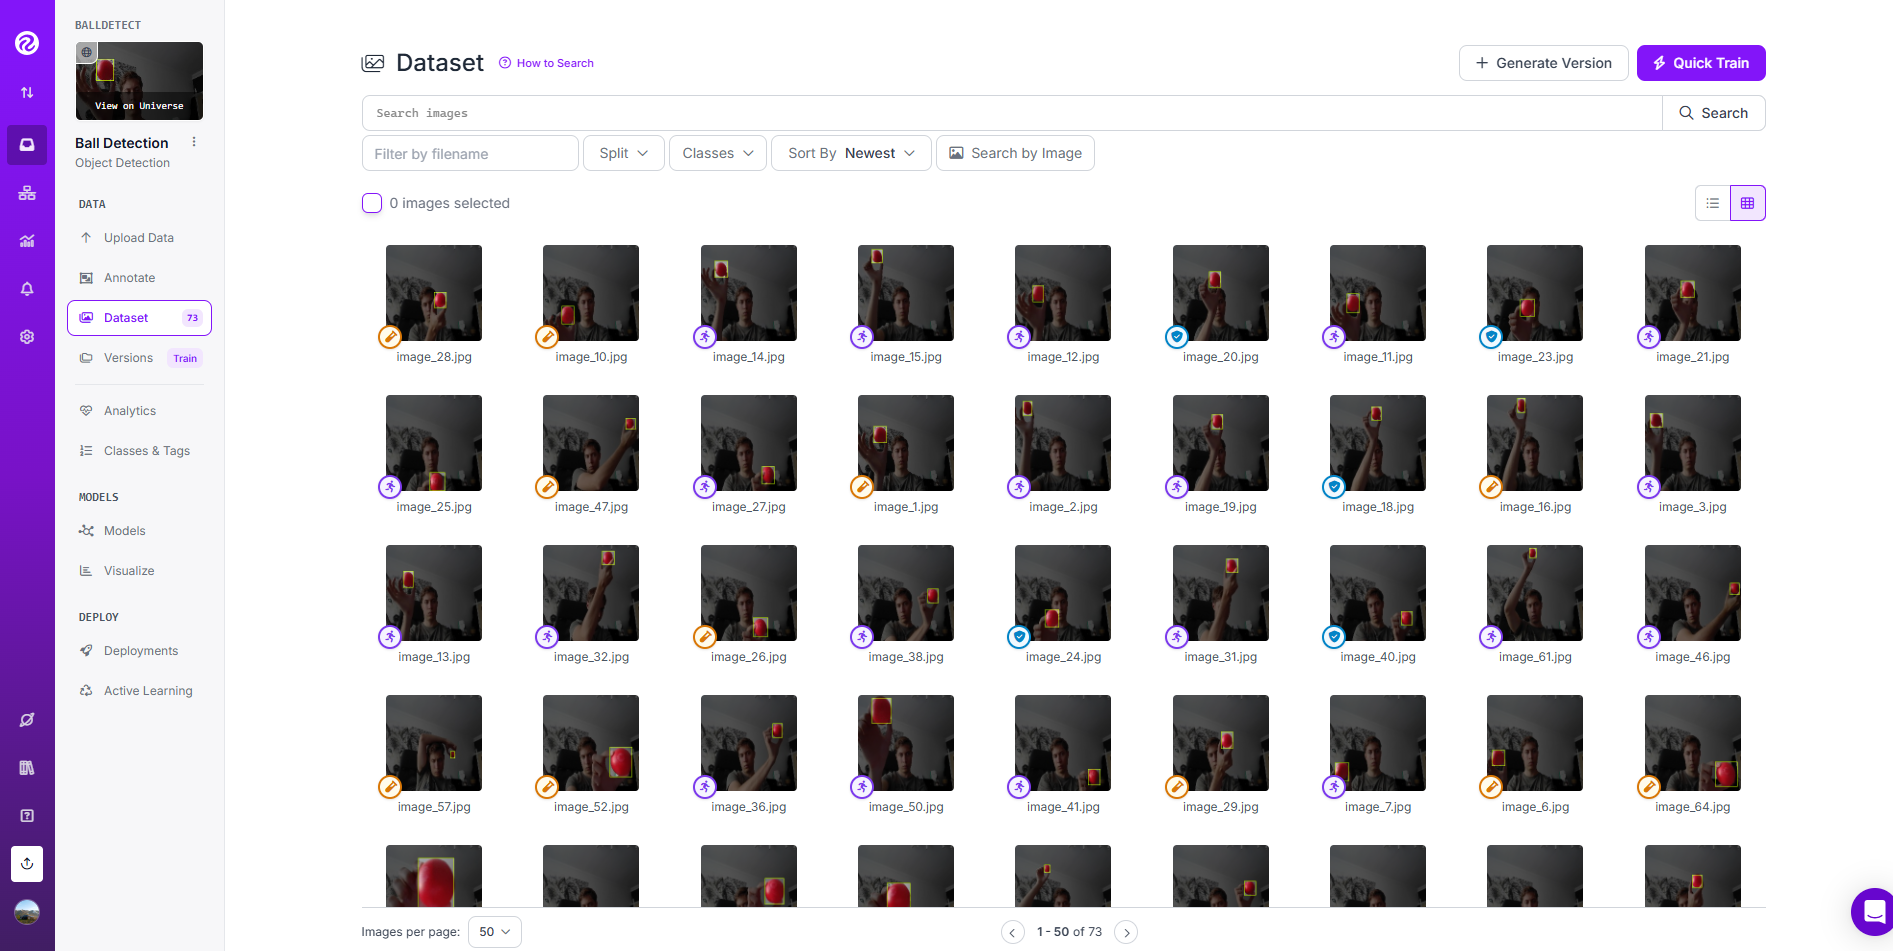
\includegraphics[width=0.75\textwidth]{Images/Roboflow/mainscreen.png}
	\caption{Widok strony głównej witryny Roboflow.}
	\label{fig:roboflow-main}
\end{figure}

Proces etykietowania danych można przeprowadzić na dwa sposoby. Pierwszy z nich to automatyczne etykietowanie, które wykorzystuje algorytmy detekcji obiektów w celu przyspieszenia oznaczania danych. Drugi sposób to etykietowanie ręczne, które polega na samodzielnym zaznaczaniu obiektów na obrazie przez użytkownika. Chociaż proces ręczny jest bardziej czasochłonny, zapewnia większą kontrolę nad poprawnością oznaczeń, co jest szczególnie istotne w przypadku trudnych warunków, takimi jak rozmyte obrazy czy słabe oświetlenie..

\newpage

\paragraph{Zdjęcie \ref{fig:labeling1}}
przedstawia interfejs użytkownika podczas etykietowania obiektów. Na obrazie widoczna jest czerwona piłka, która została zaznaczona ramką ograniczającą oraz nadano jej klasę \textbf{Ball} (oznaczającą piłkę).

\begin{figure}[h]
	\centering
	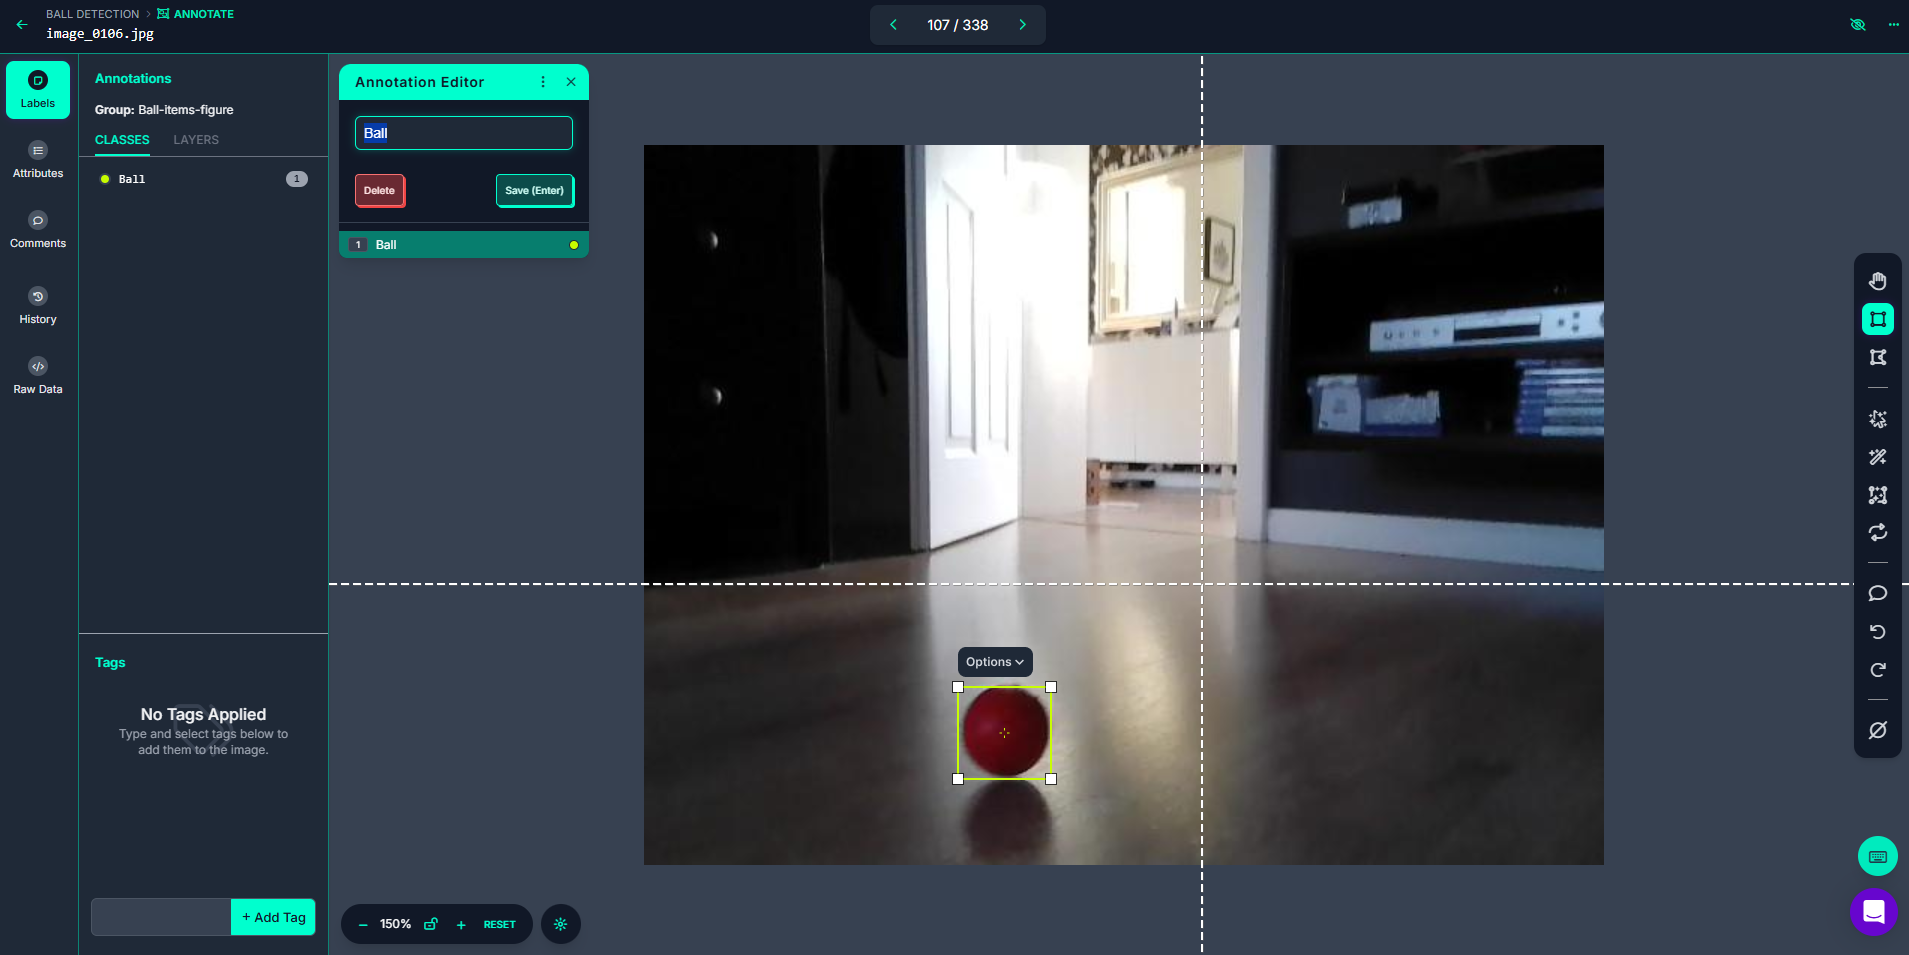
\includegraphics[width=0.75\textwidth]{Images/Roboflow/labeling1.png}
	\caption{Etykietowanie obiektów za pomocą witryny Roboflow.}
	\label{fig:labeling1}
\end{figure}

\paragraph{Zdjęcie \ref{fig:labeling3}}
pokazuje proces etykietowania w warunkach słabego oświetlenia. Pomimo trudnych warunków, obiekt został poprawnie oznaczony, co świadczy o zalecie ręcznego etykietowania w takich przypadkach.

\begin{figure}[h]
    \centering
    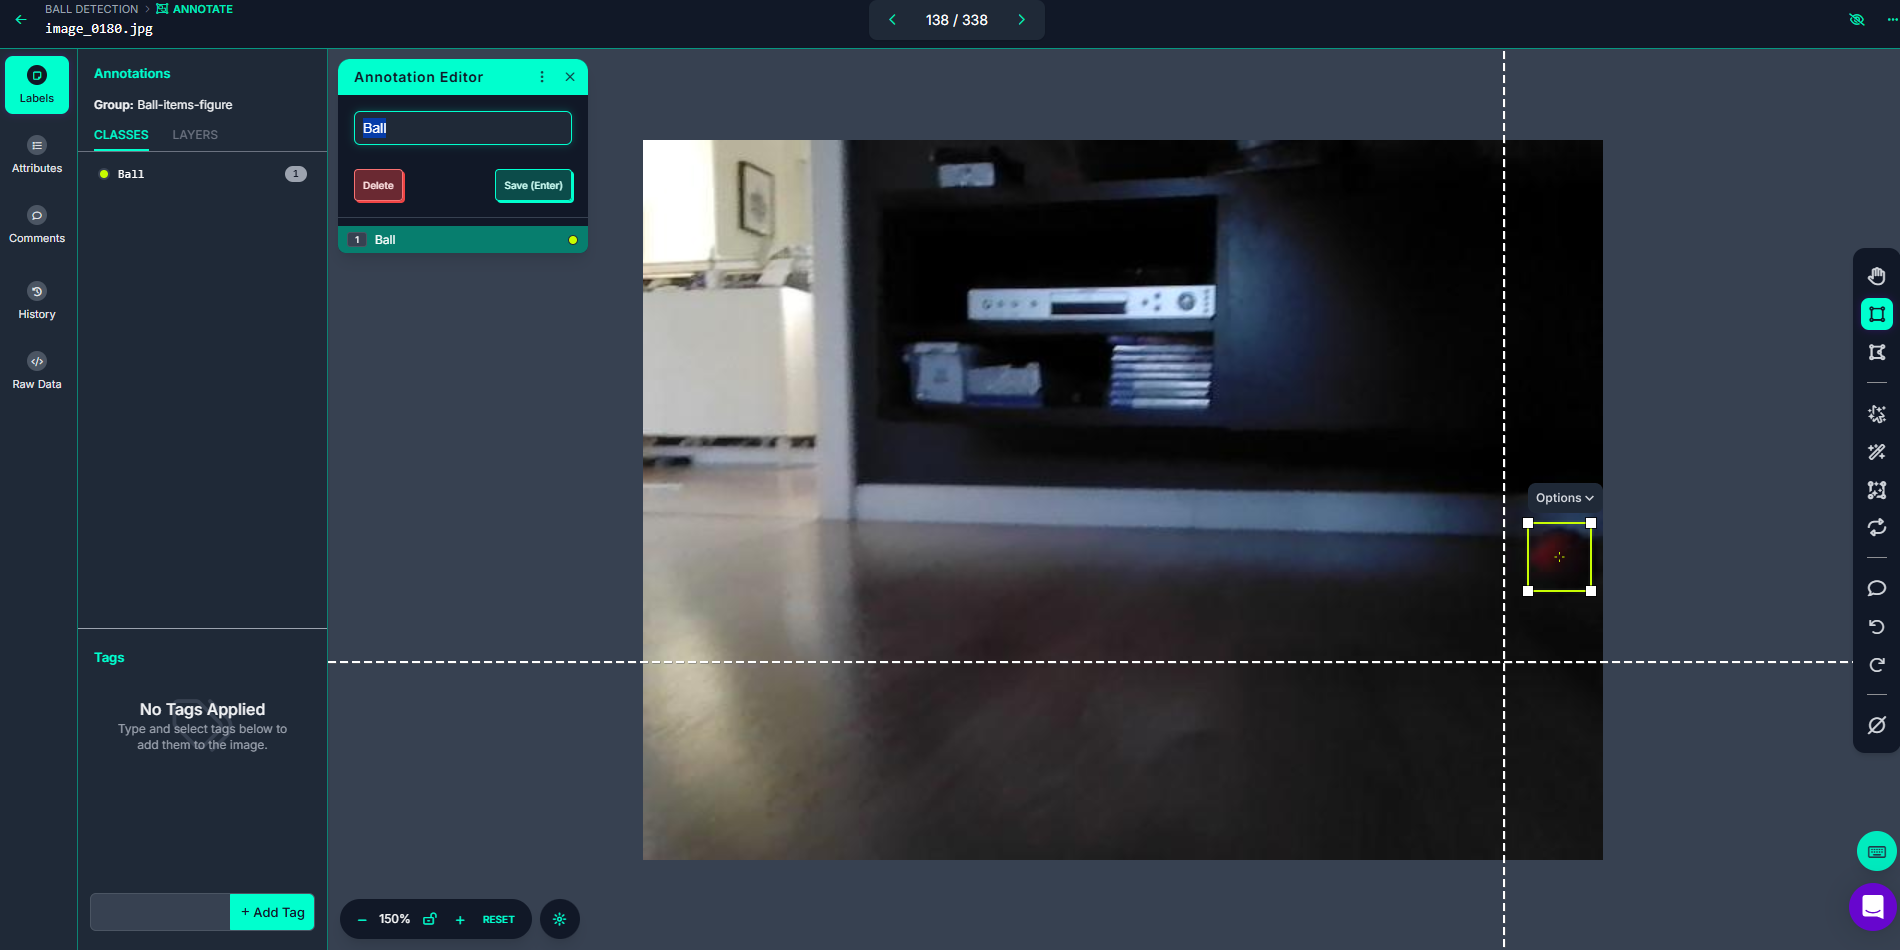
\includegraphics[width=0.75\textwidth]{Images/Roboflow/labeling3.png}
    \caption{Etykietowanie w słabym oświetleniu.}
    \label{fig:labeling3}
\end{figure}

\newpage

\subsection{Trening zestawu danych}
Po zakończeniu etykietowania danych, przystąpiono do segmentacji zbioru na zbiór treningowy, walidacyjny i testowy.
Następnie przeprowadzono trening danych aby można było wyeksportować je w formacie YOLO.
Na wykresie \ref{fig:Wykrespoczatek} przedstawiono przebieg treningu w pierwszych epokach. Widać, że wartość funkcji straty maleje wraz z postępem uczenia, co świadczy o skuteczności procesu.

\begin{figure}[h]
    \centering
    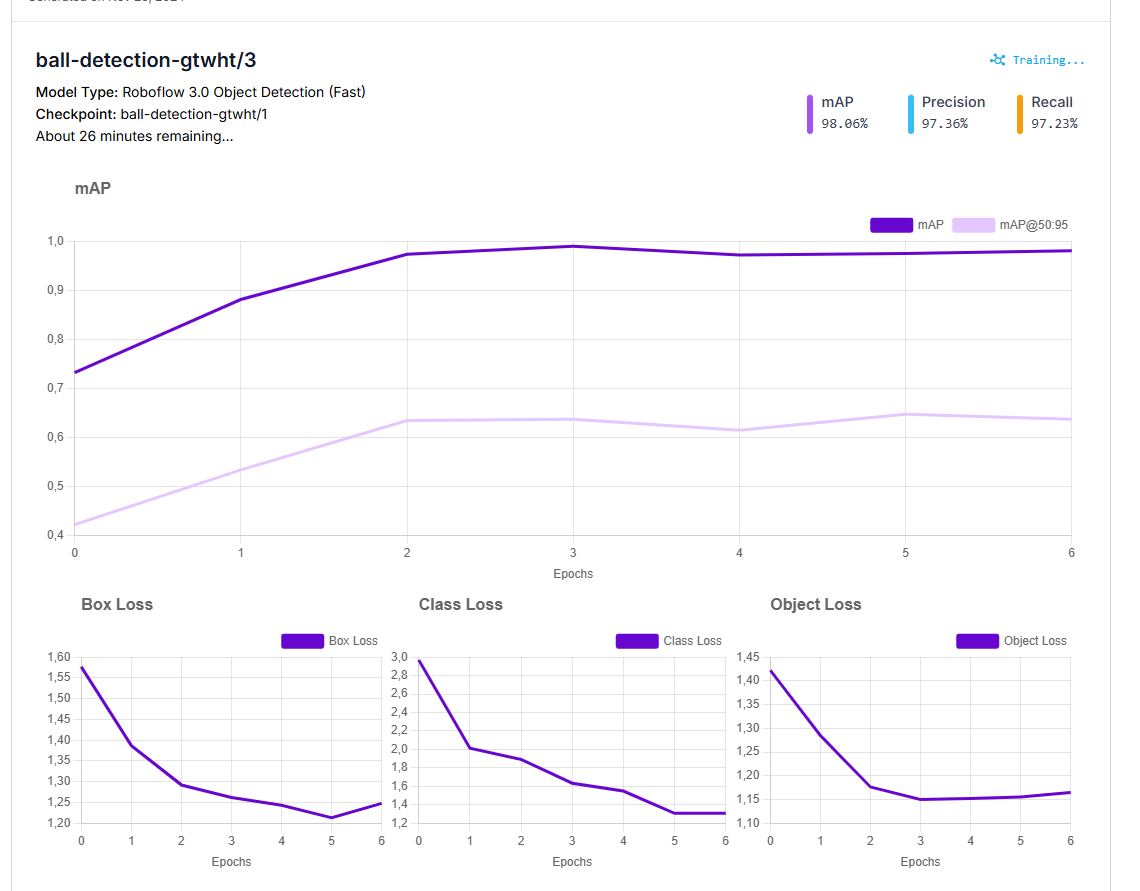
\includegraphics[width=0.75\textwidth]{Images/Roboflow/poczatek uczenia.png}
    \caption{Wykres pierwszych epok treningu.}
    \label{fig:Wykrespoczatek}
\end{figure}

\newpage

\section{Trening modelu YOLO}

Po przygotowaniu danych treningowych przystąpiono do wytrenowania modelu detekcji obiektów YOLO, korzystając z platformy Google Colab. Umożliwia ona wykorzystanie zasobów obliczeniowych w chmurze, w tym akceleracji przez GPU (ang. \textit{Graphics Processing Unit}), które znacząco przyspiesza przetwarzanie dużych ilości danych dzięki równoległemu wykonywaniu obliczeń. Jest to szczególnie istotne w przypadku modeli uczenia maszynowego, takich jak głębokie sieci neuronowe, które wymagają intensywnych operacji macierzowych. Proces treningu przebiegał zgodnie z następującymi krokami:

\subsection{Przygotowanie środowiska}
Utworzonie nowego projektu w Google Colab i skonfigurowanie środowiska do korzystania z GPU:
\begin{enumerate}
    \item Z pasku narzędzi \texttt{Środowisko wykonawcze} wybrano opcję \texttt{Zmień typ środowiska wykonawczego}.
    \item Jako \texttt{Akcelerator sprzętowy} ustawiono \texttt{GPU}.
\end{enumerate}

\subsection{Instalacja wymaganych bibliotek}
Pobranie repozytorium YOLOv7 z platformy GitHub oraz zainstalowano niezbędne zależności:
\begin{verbatim}
!git clone https://github.com/WongKinYiu/yolov7
%cd yolov7
!pip install -r requirements.txt
\end{verbatim}

\subsection{Pobranie i przygotowanie danych treningowych}
Dane treningowe zostały przygotowane na platformie Roboflow, gdzie wygenerowano klucz API, który umożliwił automatyczne pobranie danych do środowiska Google Colab. W notebooku dodano poniższy fragment kodu do zaimportowania danych:
\begin{verbatim}
!pip install roboflow
from roboflow import Roboflow
rf = Roboflow(api_key="TWÓJ_KLUCZ_API")
project = rf.workspace().project("nazwa-projektu")
dataset = project.version(1).download("yolov7")
\end{verbatim}

\subsection{Przygotowanie modelu}
Pobranie wstępnie wytrenowanych wag modelu YOLOv7:
\begin{verbatim}
!wget https://github.com/WongKinYiu/yolov7/releases/download/v0.1/yolov7.pt
\end{verbatim}

\subsection{Trening modelu}
Model wytrenowano, uruchamiając poniższą komendę:
\begin{verbatim}
%env WANDB_MODE=disabled
!python yolov7/train.py --data Ball-Detection-3/data.yaml 
--cfg yolov7/cfg/training/yolov7.yaml 
--weights yolov7.pt --epochs 50 --batch-size 16 --device 0
\end{verbatim}

Parametry treningu były następujące:
\begin{itemize}
    \item \texttt{--data}: Ścieżka do pliku konfiguracyjnego zestawu danych otrzymanych z Roboflow.
    \item \texttt{--cfg}: Plik konfiguracyjny architektury modelu.
    \item \texttt{--weights}: Wstępnie wytrenowane wagi modelu YOLOv7.
    \item \texttt{--epochs}: Liczba epok (ustawiono na 50).
    \item \texttt{--batch-size}: Rozmiar grupy treningowej (ustawiono na 16).
    \item \texttt{--device}: GPU (0 oznacza pierwsze dostępne GPU).
\end{itemize}

Epoka (ang. \textit{epoch}) to jeden pełny przebieg przez cały zbiór treningowy w procesie uczenia modelu. Podczas każdej epoki model widzi wszystkie dane treningowe przynajmniej raz i dostosowuje swoje wagi na podstawie obliczonego błędu. W tym treningu wybrano 50 epok, co oznacza, że zbiór danych treningowych został przetworzony 50 razy.

Po zakończeniu treningu najlepsze wagi modelu są zapisywane w pliku \texttt{best.pt} w folderze \texttt{runs}. Plik ten będzie wykorzystywany w programie do detekcji obiektu w czasie rzeczywistym. Dodatkowo należy pobrać foldery \texttt{models} oraz \texttt{utils} z repozytorium YOLOv7 i umieścić je w folderze z projektem.


% TODO
\chapter{Proces tworzenia robota mobilnego}
\label{ch:04}
W niniejszym rozdziale przedstawiono proces tworzenia robota mobilnego, uwzględniający zarówno założenia logiczne, jak i aspekty techniczne związane z budową oraz implementacją systemów sterowania. W pierwszej części opisano kluczowe założenia projektowe oraz schemat blokowy algorytmu robota mobilnego opartego na systemie wizyjnym. Następnie zaprezentowano proces konstrukcji robota, opierając się na modelu 3D stworzonym w programie Autodesk Fusion, oraz przedstawiono wykorzystane moduły i sposób ich podłączenia za pomocą schematu blokowego. W ostatniej części rozdziału opisano dostosowanie jednostki sterującej w postaci Raspberry Pi, w tym konfigurację niezbędnych bibliotek umożliwiających integrację podzespołów i realizację funkcjonalności systemu wizyjnego dla robota mobilnego.

\section{Założenia logiczne}
Poniżej przedstawiono diagram blokowy ilustrujący działanie algorytmu detekcji obiektów w czasie rzeczywistym. Proces rozpoczyna się od akwizycji obrazu z kamery, który następnie trafia do modelu detekcji obiektów YOLOv7. Na podstawie wyników detekcji robot dostosowuje kąty serwomechanizmów pionowego i poziomego, aby utrzymać obiekt w centrum kadru. Jeśli obiekt przesunie się poza wyznaczone centrum, program oblicza różnicę w pikselach i przelicza ją na odpowiednie wartości kątowe, umożliwiając sterowanie serwomechanizmami w celu zapewnienia ciągłości śledzenia. Celem algorytmu jest nieustanne utrzymanie obiektu w centrum widoku kamery.
Program na bieżąco monitoruje wartości kątowe serwomechanizmów, które są wykorzystywane do sterowania pracą silników DC odpowiedzialnych za ruch robota. Ruch w przód wykonywany jest jedynie w przypadku spełnienia następujących warunków: obiekt został wykryty, kąt serwomechanizmu poziomego mieści się w zakresie od -25\textdegree{} do 25\textdegree{}, a kąt serwomechanizmu pionowego przekracza -30\textdegree{}. W przeciwnym razie robot zatrzymuje się lub wykonuje skręt. Jeśli kąt poziomy osiągnie wartość graniczną (25\textdegree{} lub -25\textdegree{}), robot skręca odpowiednio w prawo lub w lewo.

Program można zatrzymać wyłącznie przez interakcję użytkownika, co powoduje zatrzymanie wszystkich systemów i powrót robota do stanu początkowego. Stan początkowy definiuje sytuację, w której serwomechanizmy ustawione są w pozycji centralnej (0\textdegree{} dla obu osi), a silniki DC są wyłączone. Dodatkowo jeśli program przestał wykrywać obiekt, przechodzi w stan poszukiwania obracając kamerą w taki sposób, że wykonuje ona ruchy eliptyczne w przestrzeni.

\begin{figure}[h]
    \centering
    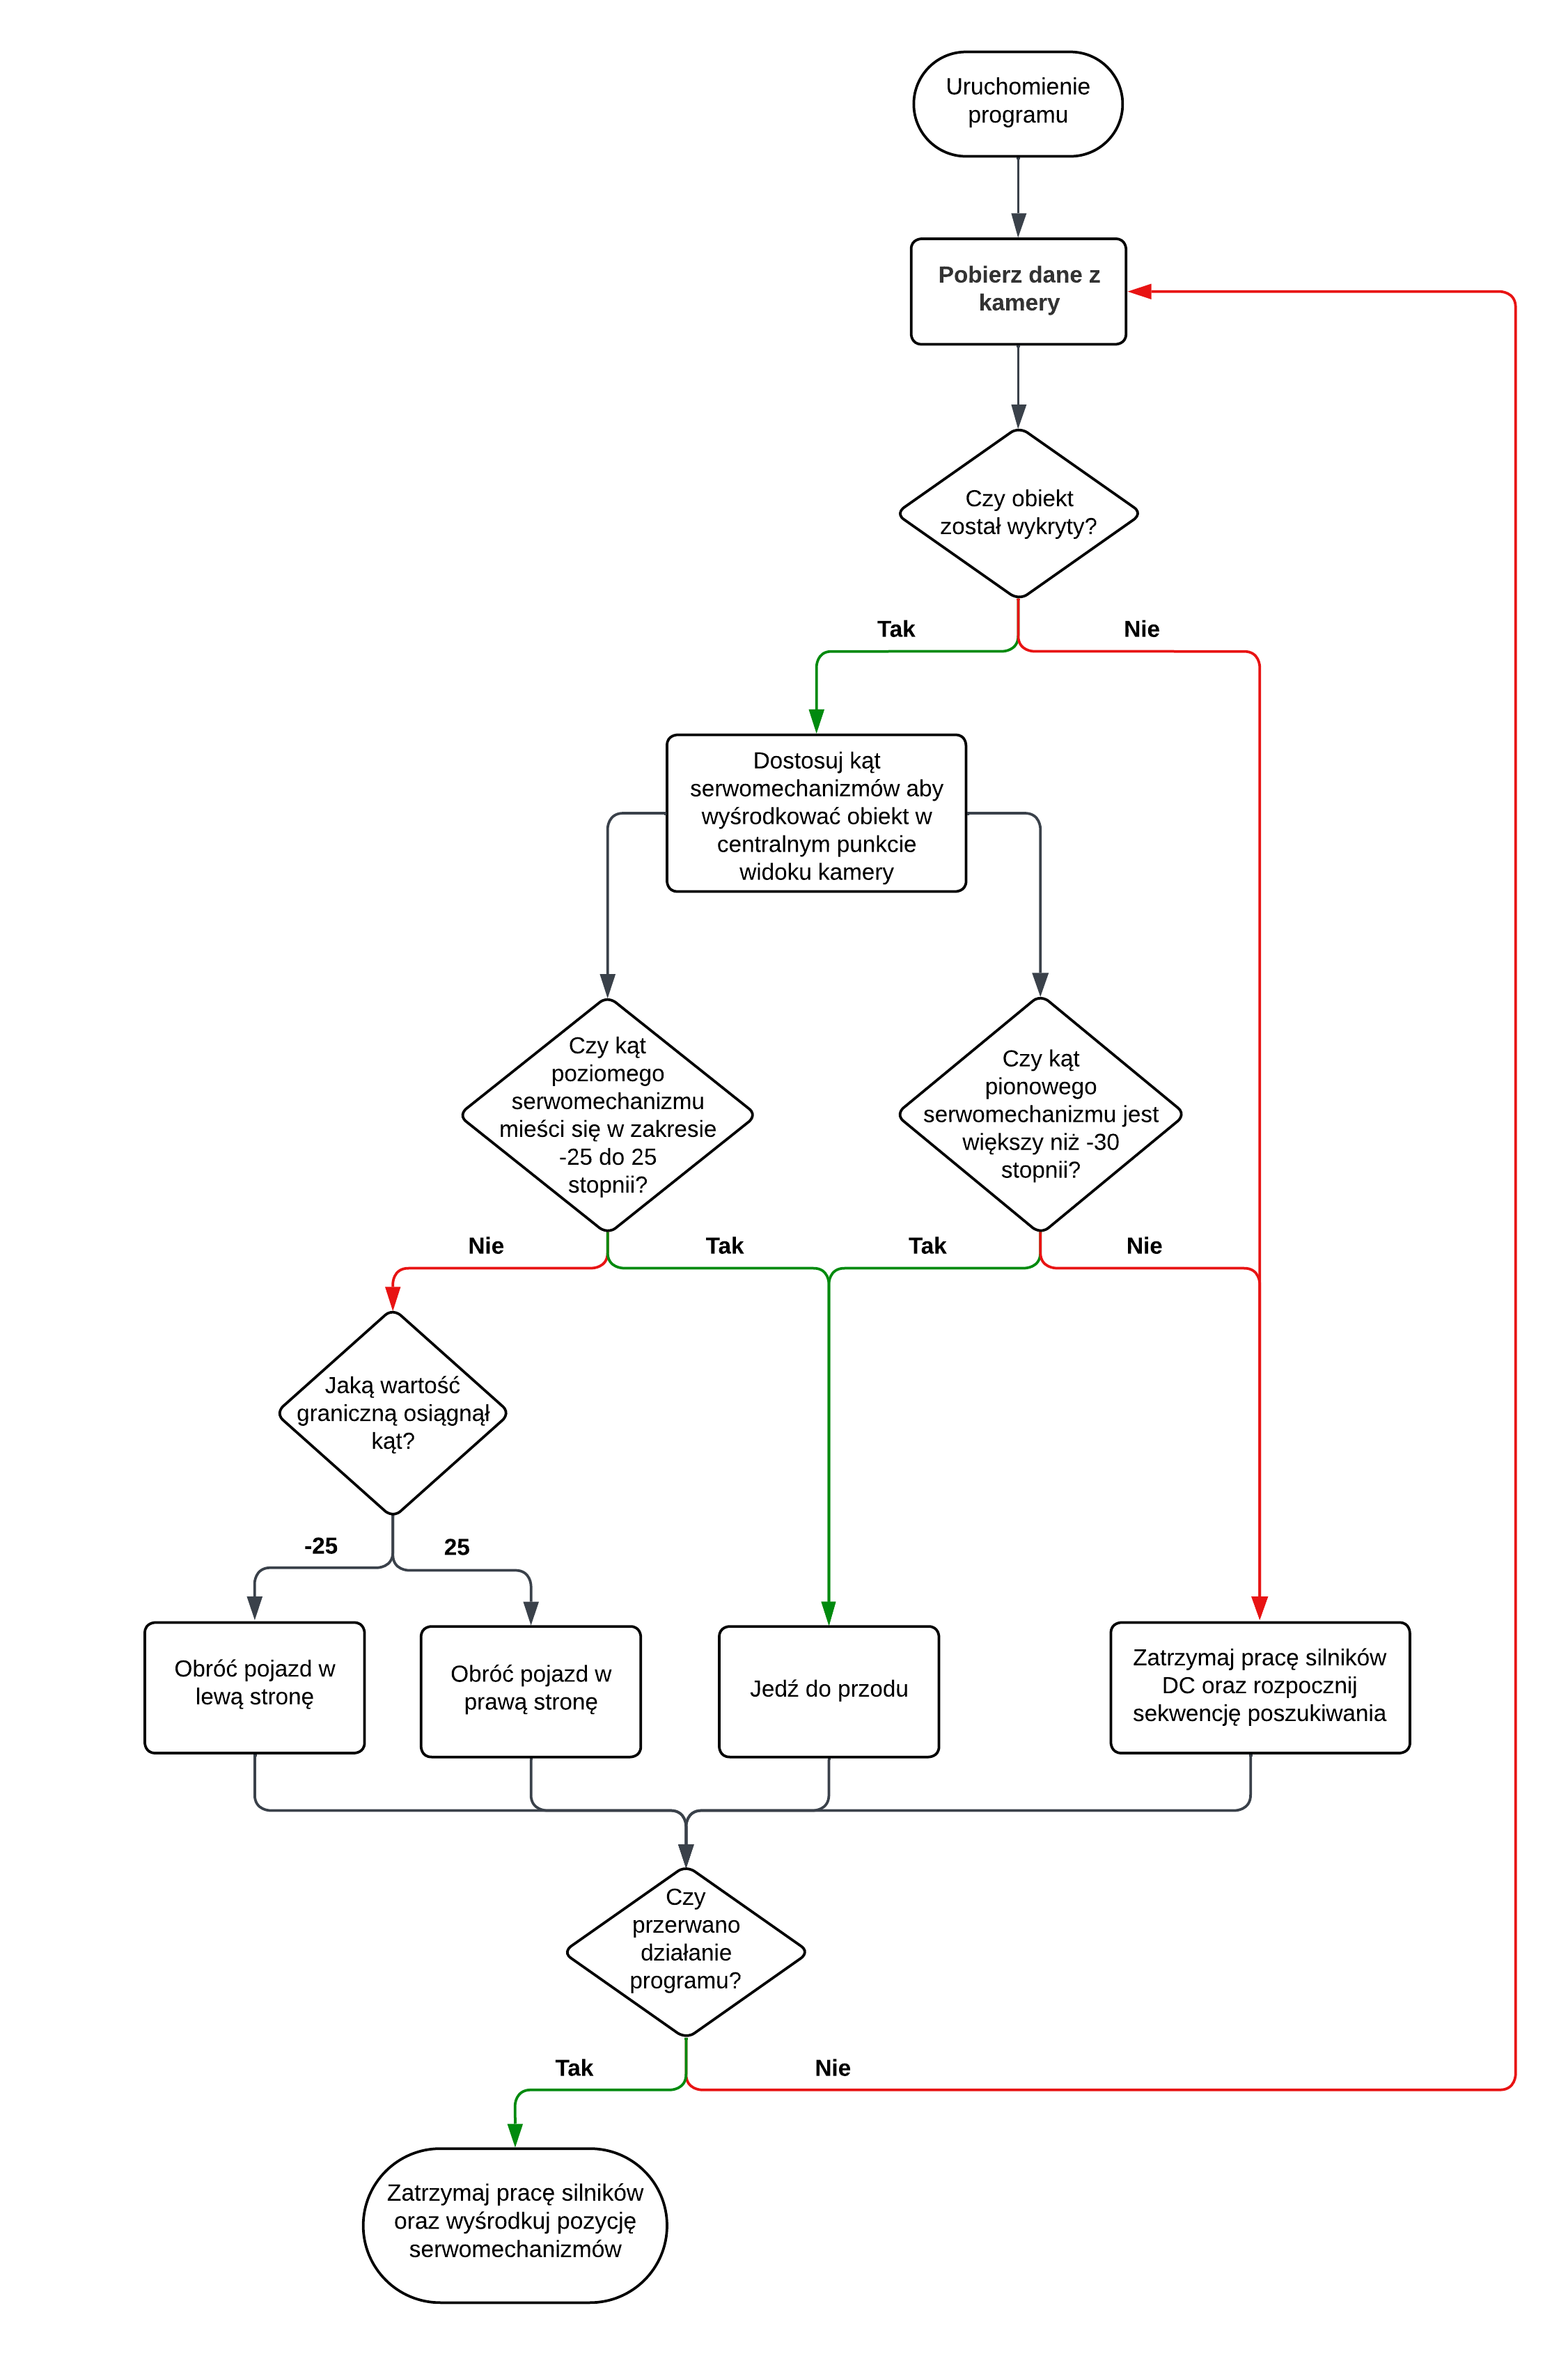
\includegraphics[width=0.75\textwidth]{Images/Schemat blokowy/Engineering Thesis.png}
    \caption{Schemat blokowy działania algorytmu pracy robota z systemem wizyjnym}
    \label{fig:Schemat blokowy}
\end{figure}

\newpage
\section{Konstrukcja robota mobilnego}
Konstrukcja robota mobilnego oparta jest na platformie jezdnej z dwoma silnikami DC o napędzie różnicowym, serwomechanizmem pionowym i poziomym oraz kamerą. Robot wyposażony jest w moduł Raspberry Pi 4B, który pełni rolę jednostki decyzyjnej oraz komunikacyjnej. Poniżej przedstawiono schemat blokowy robota mobilnego z zaznaczonymi podstawowymi elementami składowymi.

\subsection{Wykorzystane moduły}
Aby zrealizować założenia projektowe, wykorzystano następujące moduły i komponenty:
\begin{itemize}
    \item \textbf{Raspberry Pi:} Raspberry Pi 4B WiFi 8GB RAM - jednostka centralna robota, odpowiedzialna za przetwarzanie obrazu, sterowanie silnikami oraz serwomechanizmami.
    \item \textbf{Kamera:} Raspberry Pi Camera HD v3 12MPx, służąca do akwizycji obrazu.
    \item \textbf{Moduł sterownika silników:} Cytron HAT-MDD10 - dwukanałowy sterownik silników DC 24V/10A z funkcją PWM służący jako nakładka na Raspberry Pi.
    \item \textbf{Silniki DC:} Dwa silniki z przekładnią 37Dx68L 30:1 12V 330RPM + enkoder CPR 64 - Pololu 4752 - napędzające koła robota.
    \item \textbf{Zasilanie:} Cztery ogniwa 18650 Li-Ion Samsung INR18650-35E 3500mAh 3,6V - zasilanie silników DC.
    \item \textbf{Serwomechanizm pionowy:} Serwo TowerPro SG-90 micro 180 stopni - odpowiada za regulację kąta nachylenia kamery w pionie.
    \item \textbf{Serwomechanizm poziomy:} Serwo TowerPro SG-92R micro - odpowiada za regulację kąta obrotu kamery w poziomie.
    \item \textbf{Uchwyt kamery:} Wykonany z połączenia gotowego uchwytu do serw micro Pan/Tilt oraz dedykowanego uchwytu do kamery Raspberry Pi v2 oraz v3.
    \item \textbf{Obudowa:} Wykonana przy pomocy drukarki 3D z wytrzymałego filamentu Spectrum PETG 1,75mm.
    \item \textbf{Koła:} Dwa Koła Polulu 90x10mm - Zapewniające ruch robota po powierzchni.
    \item \textbf{Zasilanie Raspberry Pi:} Powerbank o parametrach 30000mAh 5V 3A.
    \item \textbf{Mocowanie silników:} Dwie sztuki mocowań aluminiowych do silników 37D Pololu 1084. 
    \item \textbf{Huby mocujące:} Dwa aluminiowe huby mocujące 6mm M3 do kół Pololu 1999.
    \item \textbf{Koło wspornikowe pasywne:} Ball Caster 3/4'' metalowe Pololu 955 - zapewniające stabilność robota.
    \item \textbf{Taśma do kamery:} Taśma Raspberry Pi kamera 60cm 15 żyłowa raster 1mm - łącząca kamerę z Raspberry Pi.
    \item \textbf{Przewody:} Zestaw przewodów połączeniowych justPi męsko-męskich, żeńsko-żeńskich, żeńsko-męskich.
    \item \textbf{Przełącznik:} Przełącznik dźwigniowy ON-OFF KN3(C)-101 250V/6A - służący do ręcznego wyłączania zasilania silników DC.
\end{itemize}

\newpage
\subsection{Schemat elektryczny}
\begin{figure}[h]
    \centering
    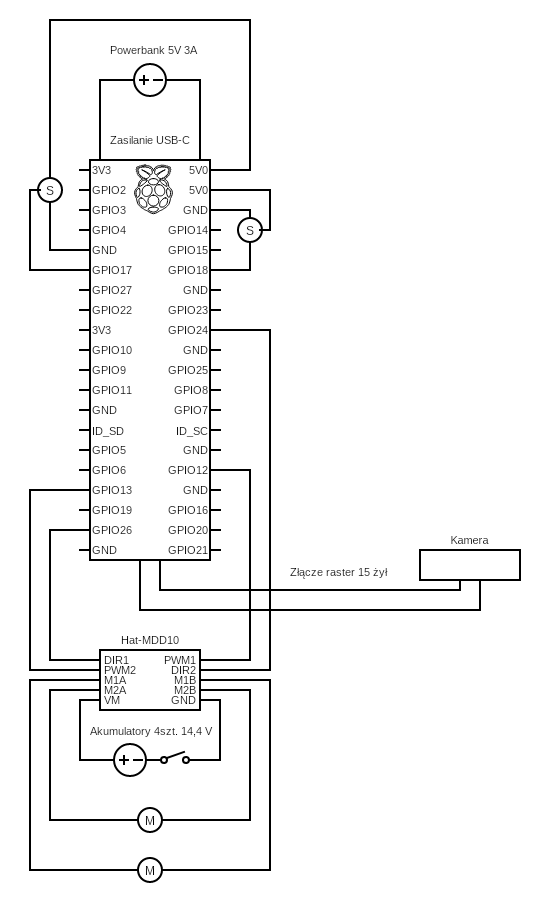
\includegraphics[width=0.6\textwidth]{Images/Schemat elektryczny/circuit.png}
    \caption{Schemat elektryczny podłączeń komponentów.}
    \label{fig:Schemat elektryczny}
\end{figure}
\newpage
\paragraph{Symbol M:} Symbolami M oznaczo silniki DC. Każdy z silników jest podłącząny ze sterownikiem Hat-MDD10 dwoma przewodami: czerwonym (dodatnim) do pinu M1A lub M2A oraz czarnym (ujemnym) do pinu M1B lub M2B.
\paragraph{Symbol S:} Symbolami S oznaczono serwomechanizmy. Serwomechanizmy podpięte są bezpośrednio do Raspberry Pi trzema przewodami - czerwonym (dodatnim) do pinu 5V, brązowym (ujemnym) do pinu GND oraz pomarańczowym (sygnałowym) do pinu GPIO.
\paragraph{Kamera:} Kamera podłączona jest do Raspberry Pi za pomocą piętnastożyłowej taśmy, która łączy się z portem CSI (ang. \texttt{Camera Serial Interface}).
\paragraph{Hat-MDD10:} Wedle instrukcji producenta \cite{bib:hatmdd10manual}, sterownik silników DC podłączony jest do Raspberry Pi za pomocą czterech przewodów do pinów GPIO1, GPIO2, PWM1 oraz PWM2. Z uwagi iż to zastosowanie powodowało asynchroniczne działanie silników DC, zdecydowano się na podłączenie sterownika z modułem Raspberry Pi w sposób nakładkowy.
\paragraph{Powerbank 5V 3A:} Powerbank podłączony jest do Raspberry Pi za pomocą przewodu USB typu A - USB typu C.
\paragraph{Akumulatory 18650:} Cztery ogniwa litowo-jonowe podłączone są szeregowo bezpośrednio do sterownika Hat-MDD10 dają łączne maksymalne napięcie 14,4V.
\paragraph{Przełącznik:} Przełącznik dźwigniowy ON-OFF przerywający ujemny przewód łączący akumulatory z Hat-MDD10.
\paragraph{RaspberryPi:} Moduł Raspberry Pi 4B zasilany z powerbanku 5V 3A oraz podłączony ze sterownikiem Hat-MDD10 w sposób nakładkowy.
\newpage
\subsection{Projekt robota mobilnego}
Jednym z założeń projektu było stworzenie kompaktowego robota mobilnego o możliwie prostym i modułowym układzie konstrukcyjnym. Robot składa się z dwóch pięter: dolnego pełniącego funkcję napędową oraz górnego będącego platformą dla modułów sterujących. Rysunek \ref{fig:Robot projekt} przedstawia projekt konstrukcji robota wykonany w programie Autodesk Fusion, widoczne na nim strzałki oznaczają kierunki obrotu serwomechanizmów oraz całej platformy mobilnej.
\begin{figure}[h]
    \centering
    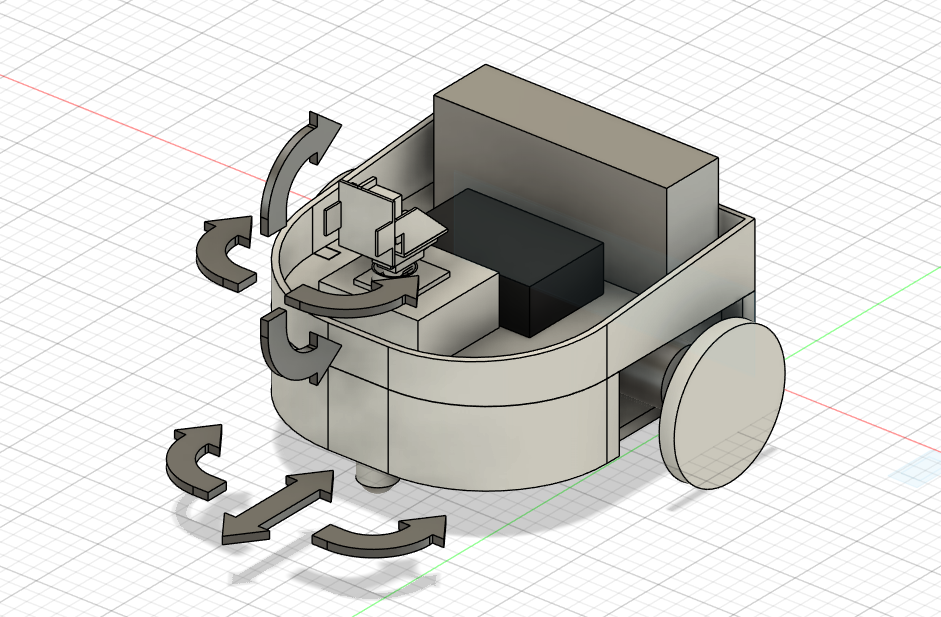
\includegraphics[width=0.6\textwidth]{Images/Robot/Robot kierunki.png}
    \caption{Projekt konstrukcji robota mobilnego wykonany w programie Autodesk Fusion.}
    \label{fig:Robot projekt}
\end{figure}
\begin{figure}[h]
    \centering
    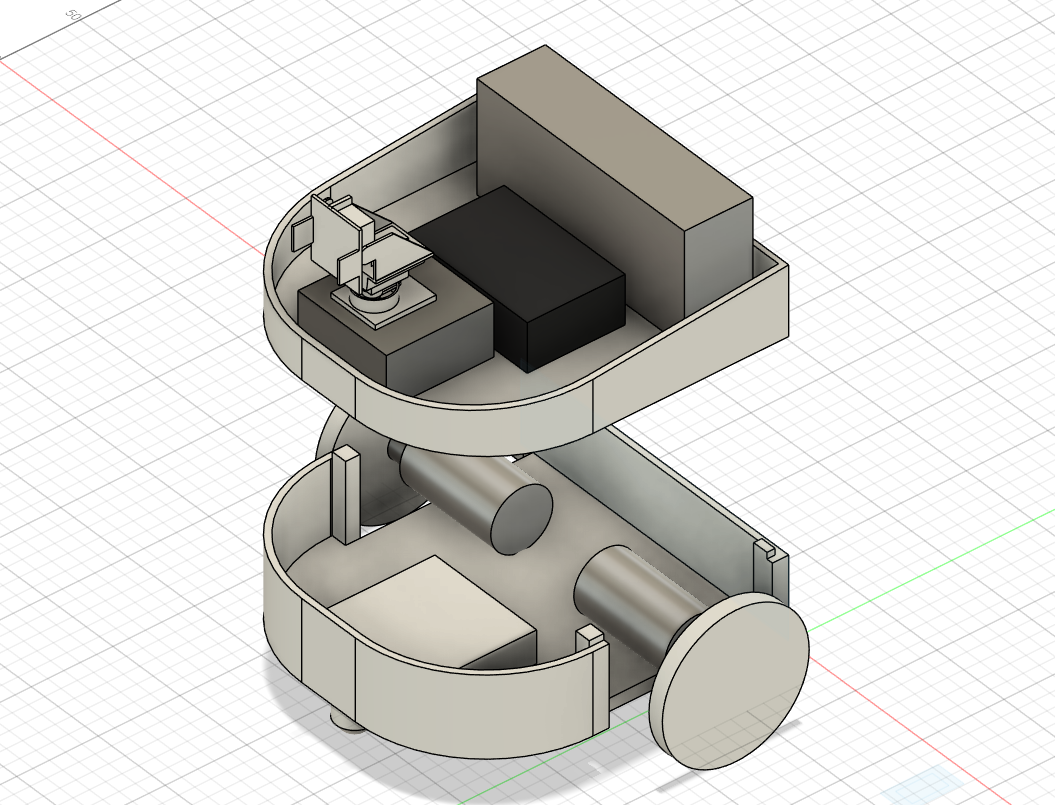
\includegraphics[width=0.6\textwidth]{Images/Robot/Robot piętra.png}
    \caption{Podział konstrukcji na piętra.}
    \label{fig:Robot piętra}
\end{figure}

\newpage
Obraz \ref{fig:Robot dół} przedstawia dolne piętro robota, na którym zamontowane są:
\begin{enumerate}
    \item Przełącznik dźwigniowy ON-OFF
    \item Silniki DC
    \item Koszyk na cztery ogniwa 18650
    \item Koła Polulu
\end{enumerate}
\begin{figure}[h]
    \centering
    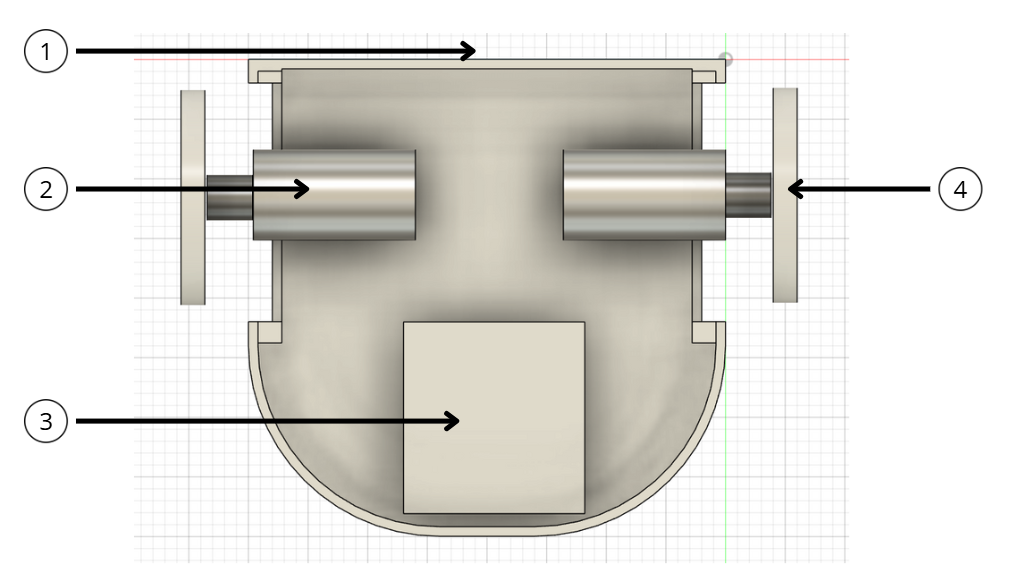
\includegraphics[width=0.9\textwidth]{Images/Robot/Robot dół oznaczenia.png}
    \caption{Widok rzutu górnego na piętro odpowiedzialne za napęd robota.}
    \label{fig:Robot dół}
\end{figure}
\newpage
Obraz \ref{fig:Robot góra} przedstawia górne piętro robota, na którym zamontowano:
\begin{enumerate}
    \item Zasilanie RaspberryPi w postaci powerbanku
    \item Połączony moduł RaspberryPi z Hat-MDD10
    \item Odważnik, którego celem jest stabilizacja robota
    \item Uchwyt na kamerę RaspberryPi wraz zamocowanymi serwomechanizmami.
    \item Kamera
\end{enumerate}
\begin{figure}[h]
    \centering
    \includegraphics[width=0.9\textwidth]{Images/Robot/Robot góra oznaczenia.png}
    \caption{Widok rzutu górnego na piętro odpowiedzialne za sterowanie robotem.}
    \label{fig:Robot góra}
\end{figure}
\newpage
Zdjęcie \ref{fig:Robot_gotowy} przedstawia gotową konstrukcję robota mobilnego wykonanego z tworzywa sztucznego PETG. 
\begin{figure}[h]
    \centering
    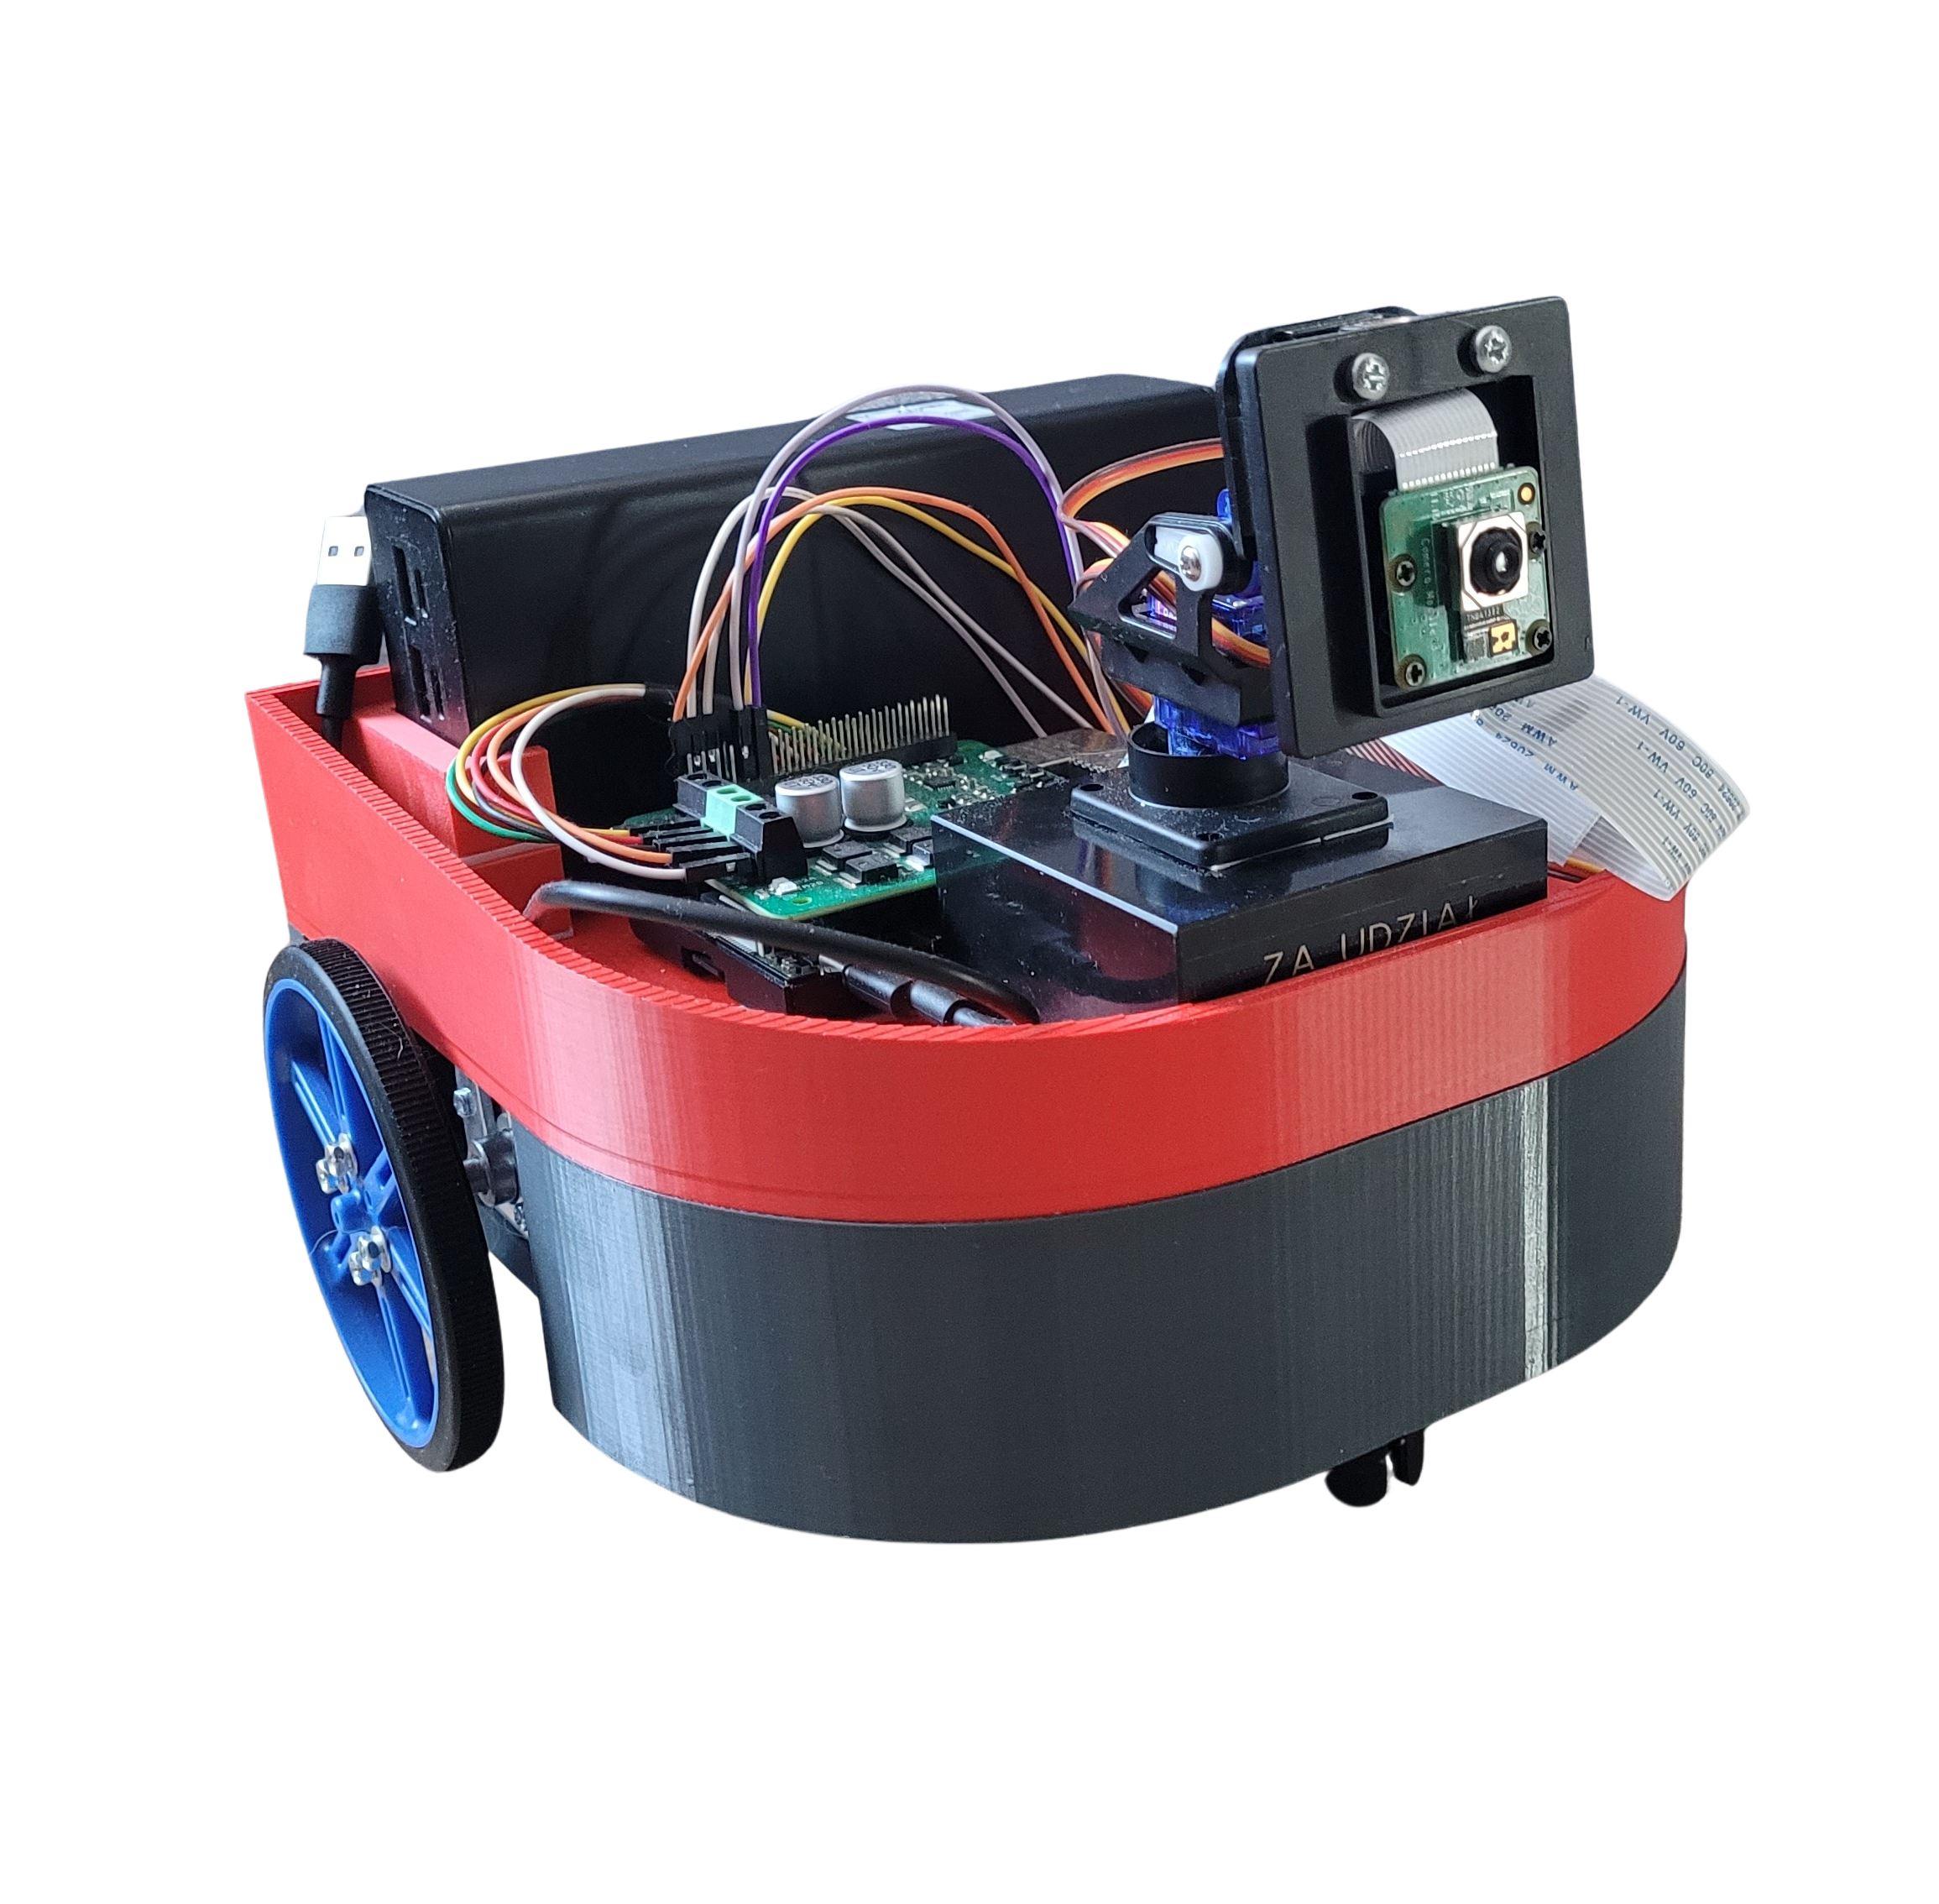
\includegraphics[width=0.6\textwidth]{Images/Robot/Robot_gotowy.png}
    \caption{Gotowa konstrukcja robota mobilnego.}
    \label{fig:Robot_gotowy}
\end{figure}

\section{Dostosowanie RaspberryPi}
Na Raspberry Pi zainstalowano system operacyjny Debian GNU/Linux 12 (Bookworm), który jest 64-bitową wersją opartą na jądrze Linux 6.6.51, zoptymalizowaną pod architekturę ARM (aarch64). Wybrana wersja systemu jest kompatybilna z bibliotekami istotnymi do poprawnego działania systemu wizyjnego. Projekt został zrealizowany w oparciu o wersję Python 3.11.2. Aby zoptymalizować pracę programu i zapewnić pełną kontrolę nad jego zależnościami, utworzono dedykowane wirtualne środowisko, w którym przechowywane są wszystkie wymagane biblioteki. Środowisko to zostało stworzone przy użyciu narzędzia \texttt{venv} za pomocą poniższego polecenia w terminalu: \begin{verbatim} python -m venv nazwa-env \end{verbatim} Po utworzeniu środowiska wirtualnego należy je aktywować, używając polecenia: \begin{verbatim} source nazwa-env/bin/activate \end{verbatim} Program jest uruchamiany wewnątrz tego środowiska, co pozwala na uniknięcie konfliktów między wersjami bibliotek oraz zapewnia powtarzalność działania systemu na różnych urządzeniach.

\newpage
\subsection{Spis wymaganych bibliotek}
Poniżej przedstawiono listę bibliotek wymaganych do uruchomienia systemu wizyjnego oraz sterowania robotem mobilnym, z podziałem na ich funkcje:

\begin{itemize}
    \item \textbf{Platformy uczenia maszynowego:}
    \begin{itemize}
        \item \textbf{torch} – Podstawowa platforma do trenowania i uruchamiania modeli uczenia maszynowego.
        \item \textbf{models.experimental} – Obsługa modeli YOLO do detekcji obiektów.
        \item \textbf{utils.general} – Funkcje wspomagające dla YOLO, takie jak filtrowanie wyników i skalowanie współrzędnych.
    \end{itemize}
    
    \item \textbf{Przetwarzanie obrazu:}
    \begin{itemize}
        \item \textbf{opencv-python} (cv2) – Obsługa obrazów i przetwarzanie wizyjne, np. binaryzacja i filtrowanie.
        \item \textbf{numpy} – Operacje matematyczne i macierzowe, kluczowe dla analizy danych wizualnych.
        \item \textbf{Picamera2} – Obsługa kamery Raspberry Pi do akwizycji obrazu.
    \end{itemize}
    \item \textbf{Sterowanie sprzętem:}
    \begin{itemize}
        \item \textbf{RPi.GPIO} – Sterowanie pinami GPIO na Raspberry Pi.
        \item \textbf{pigpio} – Niskopoziomowe sterowanie GPIO, np. dla serwomechanizmów.
    \end{itemize}
    
    \item \textbf{Inne ważne biblioteki:}
    \begin{itemize}
        \item \textbf{tqdm} – Pasek postępu przy iteracjach.
        \item \textbf{PyYAML} – Obsługa plików konfiguracji w formacie YAML.
    \end{itemize}
\end{itemize}

Szczegółowy spis wszystkich bibliotek został przedstawiony w pliku Biblioteki.txt dostarczonym w załączniku do pracy.


%\begin{figure}
%\centering
%\begin{tikzpicture}
%\begin{axis}[
%    y tick label style={
%        /pgf/number format/.cd,
%            fixed,   % po zakomentowaniu os rzednych jest indeksowana wykladniczo
%            fixed zerofill, % 1.0 zamiast 1
%            precision=1,
%        /tikz/.cd
%    },
%    x tick label style={
%        /pgf/number format/.cd,
%            fixed,
%            fixed zerofill,
%            precision=2,
%        /tikz/.cd
%    }
%]
%\addplot [domain=0.0:0.1] {rnd};
%\end{axis} 
%\end{tikzpicture}
%\caption{Podpis rysunku po rysunkiem.}
%\label{fig:2}
%\end{figure}







%\begin{figure}
%\centering
%\begin{minted}[linenos,frame=lines]{c++}
%class test : public basic
%{
%    public:
%      test (int a);
%      friend std::ostream operator<<(std::ostream & s, 
%                                     const test & t);
%    protected:
%      int _a;  
%      
%};
%\end{minted}
%\caption{Pseudokod w \texttt{minted}.}
%\label{fig:pseudokod:minted}
%\end{figure}


\chapter{Analiza działania systemu wizyjnego}
\label{ch:05}
W niniejszym rozdziale przedstawiono analizę działania systemu wizyjnego, który został zaimplementowany w ramach pracy. System ten umożliwia detekcję obiektu na obrazie z kamery Raspberry Pi, a następnie sterowanie serwomechanizmami w celu utrzymania obiektu w centrum kadru. W ramach analizy porównano skuteczność dwóch podejść do detekcji obiektów: 
\begin{itemize}
    \item model YOLOv7 oraz YOLOv8,
    \item algorytm binaryzacji obrazu z wykorzystaniem przestrzeni barw HSV,
\end{itemize}

Porównanie zostało przeprowadzone pod kątem dwóch głównych aspektów:
\begin{enumerate}
    \item \textbf{Skuteczności wykrywania obiektów:} Analizowano zdolność algorytmów do wykrywania obiektu w różnych warunkach oświetleniowych oraz w otoczeniu obiektów zakłócających.
    \item \textbf{Wydajności działania:} Mierzono czas przetwarzania obrazu w klatkach na sekundę - FPS (ang. \textit{Frames Per Second}), co pozwala określić, jak szybko algorytm jest w stanie działać na urządzeniu.
\end{enumerate}

\newpage

\section{Specyfikacja sprzętowa}
Poniżej przedstawiono specyfikację urządzeń użytych do analizy skuteczności algorytmów:
\begin{itemize}
    \item \textbf{Komputer osobisty:} Urządzenie wykorzystane do testowania algorytmu binaryzacji oraz modelów YOLO.
    \begin{itemize}
        \item \textbf{Procesor:} Intel Core i5-13500H, 12 rdzeni, taktowanie do 2.6 GHz.
        \item \textbf{Pamięć RAM:} 16 GB DDR5, taktowanie 6400 MHz.
        \item \textbf{Karta graficzna:} 
        \begin{itemize}
            \item Intel Arc A350M Graphics, 1 GB VRAM.
            \item Intel Iris Xe Graphics, 2 GB VRAM.
        \end{itemize}
        \item \textbf{System operacyjny:} Microsoft Windows 11 Home, wersja 10.0.22631, architektura 64-bit.
    \end{itemize}
    \item \textbf{Raspberry Pi:} Platforma testowa dla algorytmu binaryzacji oraz modelów YOLO.
    \begin{itemize}
        \item \textbf{Procesor:} Broadcom BCM2711 (Cortex-A72), 4 rdzenie, architektura ARMv8-A, taktowanie 1.5 GHz.
        \item \textbf{Pamięć RAM:} 8 GB LPDDR4.
        \item \textbf{System operacyjny:} Debian GNU/Linux 12 (Bookworm).
        \item \textbf{Kamera:} Raspberry Pi Camera HD v3 12MPx.
    \end{itemize}    
\end{itemize}

\section{Detekcja obiektu za pomocą narzędzi głębokiego uczenia}

W podrozdziale tym opisano podejście do detekcji obiektu (czerwonej piłki) z wykorzystaniem zaawansowanych narzędzi głębokiego uczenia, takich jak modele z rodziny YOLO (ang. \textit{You Only Look Once}).
W porównaniu do klasycznych technik przetwarzania obrazów, modele głębokiego uczenia wymagają większych zasobów obliczeniowych, ale oferują większą elastyczność i skuteczność w złożonych warunkach otoczenia.

\newpage
\subsection{Opis działania programu}

System opiera się na detekcji obiektu (piłki) w czasie rzeczywistym z wykorzystaniem modelu YOLO oraz sterowaniu ruchem robota przy pomocy serwomechanizmów i silników DC. Program realizuje funkcjonalność autonomicznego śledzenia piłki oraz reagowania na jej pozycję w kadrze kamery.

\paragraph{Wczytanie modelu}
Model YOLO, zapisany w pliku \texttt{best.pt}, jest wczytywany z użyciem funkcji \texttt{attempt\_load}. Model jest przełączany w tryb ewaluacyjny (ang. \textit{evaluation mode}), aby umożliwić jego wykorzystanie wyłącznie do predykcji. Kod odpowiedzialny za ładowanie modelu przedstawiono w \textbf{Kodzie}~\ref{lst:model_loading}.

\begin{lstlisting}[language=Python, caption={Ładowanie modelu YOLO do pamięci.}, label={lst:model_loading}, captionpos=b]
model_path = "/home/lukasgrab/GoodDetection/runs/train/ball_detection6/weights/best.pt"
device = torch.device('cpu')
model = attempt_load(model_path, map_location=device)
model.eval()
\end{lstlisting}

\paragraph{Detekcja piłki}
Podstawowa logika detekcji polega na przetwarzaniu obrazu z kamery, który jest skalowany i przetwarzany przez model YOLO. Wyniki predykcji są filtrowane za pomocą mechanizmu \textit{non-max suppression} w celu eliminacji zbędnych ramek detekcji. Po wykryciu piłki jej pozycja jest obliczana względem środka obrazu. Fragment kodu odpowiedzialny za tę funkcję przedstawiono w \textbf{Kodzie}~\ref{lst:ball_detection}.

\begin{lstlisting}[language=Python, caption={Logika detekcji piłki przy użyciu modelu YOLO.}, label={lst:ball_detection}, captionpos=b]
predictions = model(img)[0]
predictions = non_max_suppression(predictions, conf_thres=0.10, iou_thres=0.45)

for det in predictions:
    if det is not None and len(det):
        for *xyxy, conf, cls in det:
            x1, x2 = int(xyxy[0]), int(xyxy[2])
            y1, y2 = int(xyxy[1]), int(xyxy[3])
            ball_center_x = (x1 + x2) / 2
            ball_center_y = (y1 + y2) / 2
\end{lstlisting}

\newpage
\paragraph{Logika kwadratu w centrum obrazu}
W centrum obrazu rysowany jest kwadrat, który definiuje obszar uznawany za "środek obrazu". Rozmiar kwadratu został dobrany w taki sposób, aby stworzyć większy obszar stabilności dla kamery. Gdyby centrum zostało zdefiniowane jako pojedynczy piksel, nawet niewielkie ruchy obiektu wynikające z drgań kamery, zmieniających się warunków oświetleniowych lub naturalnego ruchu piłki powodowałyby ciągłą próbę korekcji pozycji przez serwomechanizmy. Taka sytuacja skutkowałaby niestabilnością układu.

Kwadrat pozwala na bardziej stabilne śledzenie, ponieważ robot uznaje piłkę za "wycentrowaną", gdy znajduje się w tym obszarze, nawet jeśli nie jest dokładnie w punkcie środkowym.

\paragraph{Definiowanie ograniczeń kątowych}
Sterowanie serwomechanizmami w programie wymagało zdefiniowania zakresów ruchu, aby uniknąć uszkodzenia mechanicznego urządzeń. Dla serwomechanizmu odpowiedzialnego za ruch poziomy (ang. \textit{pan}) przyjęto ograniczenia w zakresie od $-25^{\circ}$ do $25^{\circ}$. Z kolei serwomechanizm odpowiedzialny za ruch pionowy (ang. \textit{tilt}) może zmieniać kąt w zakresie od $-30^{\circ}$ do $30^{\circ}$. Te wartości są podyktowane fizycznymi możliwościami serwomechanizmów oraz potrzebą zapewnienia odpowiedniej elastyczności ruchu robota.

\paragraph{Przeliczanie kąta na szerokość impulsu}
Sterowanie serwomechanizmami wymaga przekształcenia kąta (w stopniach) na szerokość impulsu (ang. \textit{pulse width}) w mikrosekundach, co odpowiada wymaganiom sterownika serwomechanizmu. Proces ten realizuje funkcja przedstawiona w \textbf{Kodzie}~\ref{lst:set_servo_angle}.

\begin{lstlisting}[language=Python, caption={Przeliczanie kąta na szerokość impulsu.}, label={lst:set_servo_angle}, captionpos=b]
def set_servo_angle(pin, angle):
    pulse_width = 500 + (angle + 90) * 2000 / 180
    pi.set_servo_pulsewidth(pin, pulse_width)
\end{lstlisting}

\newpage
Funkcja \texttt{set\_servo\_angle} realizuje następujące kroki:
\begin{itemize}
    \item \texttt{angle} — kąt w stopniach, przekazywany do funkcji. Może przyjmować wartości od $-90^{\circ}$ do $90^{\circ}$.
    \item \texttt{pulse\_width} — szerokość impulsu w mikrosekundach, obliczana na podstawie wzoru:
    \begin{align}
    \texttt{pulse\_width} = 500 + \frac{(\texttt{angle} + 90) \cdot 2000}{180}
    \end{align}
    gdzie:
    \begin{itemize}
        \item $500$ — minimalna szerokość impulsu w mikrosekundach, odpowiadająca kątowi $-90^{\circ}$,
        \item $2000$ — maksymalna różnica szerokości impulsu, odpowiadająca zakresowi $180^{\circ}$,
        \item $180$ — zakres pełnych kątów ruchu serwomechanizmu ($-90^{\circ}$ do $90^{\circ}$),
        \item $\texttt{angle} + 90$ — przesunięcie kąta, aby obliczenia obejmowały pełny zakres od $0^{\circ}$ do $180^{\circ}$.
    \end{itemize}
    \item Funkcja wywołuje \texttt{pi.set\_servo\_pulsewidth}, aby ustawić odpowiednią szerokość impulsu na wybranym pinie GPIO.
\end{itemize}

\paragraph{Sterowanie serwomechanizmami}
Sterowanie serwomechanizmami realizuje dynamiczne dostosowanie kątów nachylenia w celu śledzenia pozycji piłki. Pozycja piłki w kadrze obrazu jest przekształcana na współrzędne w pikselach, a następnie na kąty dla serwomechanizmów. Kluczowy fragment kodu odpowiedzialny za sterowanie serwomechanizmami przedstawiono w \textbf{Kodzie}~\ref{lst:servo_control}.

\begin{lstlisting}[language=Python, caption={Algorytm sterowania serwomechanizmami.}, label={lst:servo_control}, captionpos=b]
new_pan_angle = current_pan_angle + (normalized_dx * 5)
new_tilt_angle = current_tilt_angle - (normalized_dy * 5)

new_pan_angle = max(MIN_ANGLE_PAN, min(MAX_ANGLE_PAN, new_pan_angle))
new_tilt_angle = max(MIN_ANGLE_TILT, min(MAX_ANGLE_TILT, new_tilt_angle))

set_servo_angle(servo_pin_pan, new_pan_angle)
set_servo_angle(servo_pin_tilt, new_tilt_angle)
\end{lstlisting}

\paragraph{Logika sterowania ruchem}
Robot realizuje ruch do przodu, gdy piłka jest wykryta i znajduje się w granicach zadanych kątów serwomechanizmów. W przypadku, gdy kąt poziomy (pan) przekroczy wartość graniczną, robot wykonuje skręt w odpowiednią stronę. Logikę sterowania ruchem przedstawiono w \textbf{Kodzie}~\ref{lst:motion_logic}.

\begin{lstlisting}[language=Python, caption={Logika sterowania ruchem robota.}, label={lst:motion_logic}, captionpos=b]
if abs(current_tilt_angle) < TILT_STOP_THRESHOLD:
    move_forward()
else:
    stop_motors()

if abs(current_pan_angle) >= PAN_TURN_THRESHOLD:
    stop_motors()
    if current_pan_angle > 0:
        turn_left()
    else:
        turn_right()
\end{lstlisting}

\paragraph{Zgubienie piłki}
Jeśli piłka nie zostanie wykryta przez określony czas, robot przechodzi w tryb szukania. W tym trybie serwomechanizmy wykonują w przestrzeni ruchy eliptyczne w celu ponownego odnalezienia obiektu. Ruch ten opiera się na funkcjach trygonometrycznych \texttt{sin} i \texttt{cos}, które generują odpowiednie kąty dla serwomechanizmów. Kluczowy fragment kodu realizujący ten mechanizm przedstawiono w Kodzie~\ref{lst:lost_ball}.

\begin{lstlisting}[language=Python, caption={Logika zgubienia piłki i ruchu eliptycznego.}, label={lst:lost_ball}, captionpos=b]
if time.time() - last_detected_time > 1:
    search_time += 0.1
    new_pan_angle = PAN_AMPLITUDE * math.cos(search_time)
    new_tilt_angle = TILT_AMPLITUDE * math.sin(search_time) + TILT_OFFSET
    new_pan_angle = max(MIN_ANGLE_PAN, min(MAX_ANGLE_PAN, new_pan_angle))
    new_tilt_angle = max(MIN_ANGLE_TILT, min(MAX_ANGLE_TILT, new_tilt_angle))

    set_servo_angle(servo_pin_pan, new_pan_angle)
    set_servo_angle(servo_pin_tilt, new_tilt_angle)
    current_pan_angle = new_pan_angle
    current_tilt_angle = new_tilt_angle
\end{lstlisting}

W powyższym kodzie:
\begin{itemize}
    \item \texttt{search\_time} — zmienna czasu, która jest inkrementowana w każdej iteracji, aby generować płynne zmiany kąta.
    \item \texttt{math.cos(search\_time)} — generuje wartości dla poziomego ruchu serwomechanizmu \textbf{pan}.
    \item \texttt{math.sin(search\_time)} — generuje wartości dla pionowego ruchu serwomechanizmu \textbf{tilt}.
    \item \texttt{PAN\_AMPLITUDE} i \texttt{TILT\_AMPLITUDE} — amplitudy ruchu poziomego i pionowego, które kontrolują zakres ruchu serwomechanizmów.
    \item \texttt{TILT\_OFFSET} — przesunięcie pionowe, aby tilt oscylował wokół ustalonej wartości.
\end{itemize}

\newpage
\subsection{Uzyskane rezultaty}
W ramach testów systemu wizyjnego przeprowadzono analizę skuteczności detekcji piłki w różnych warunkach oświetleniowych oraz w obecności obiektów potencjalnie zakłócających prawidłowe działanie algorytmu. Celem testów było zweryfikowanie odporności systemu na zmienne warunki środowiskowe oraz jego zdolności do ignorowania obiektów o zbliżonym kształcie lub barwie do śledzonej piłki.

Na \textbf{Rysunku}~\ref{fig:Wykrycie_piłki1} przedstawiono sytuację przy dobrym oświetleniu, gdzie system poprawnie wykrył piłkę czerwoną, jednocześnie ignorując inne obiekty znajdujące się w polu widzenia kamery. Natomiast na \textbf{Rysunku}~\ref{fig:Wykrycie_piłki2} zaprezentowano scenariusz przy gorszych warunkach oświetleniowych, w którym system nadal poprawnie wykrył piłkę czerwoną, jednak błędnie sklasyfikował obiekt o innej barwie jako piłkę.

\begin{figure}[!hb]
    \centering
    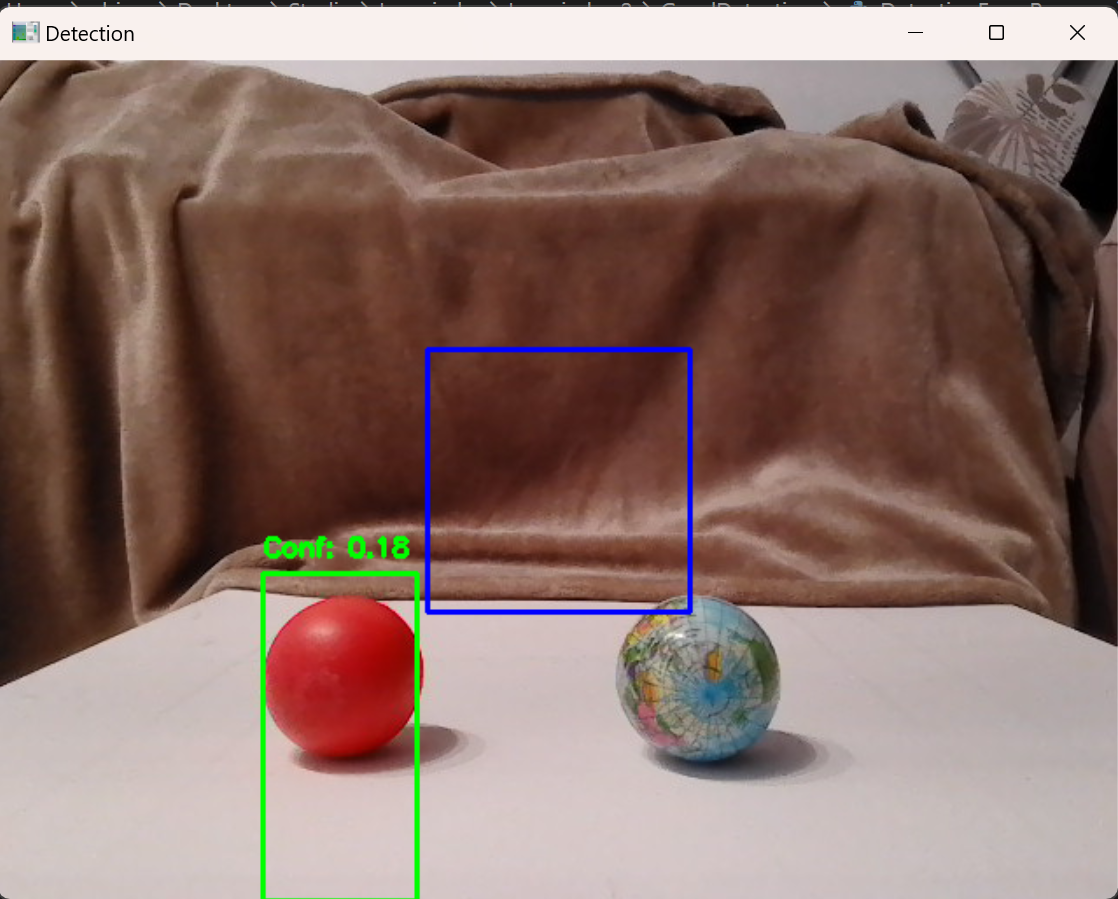
\includegraphics[width=0.5\textwidth]{Images/Porownanie/Yolo7 robot/Zrzut ekranu 2025-01-02 194147.png}
    \caption{Sytuacja przy dobrym oświetleniu — poprawne wykrycie piłki czerwonej oraz zignorowanie piłki o innych barwach.}
    \label{fig:Wykrycie_piłki1}
\end{figure}

\begin{figure}[!hb]
    \centering
    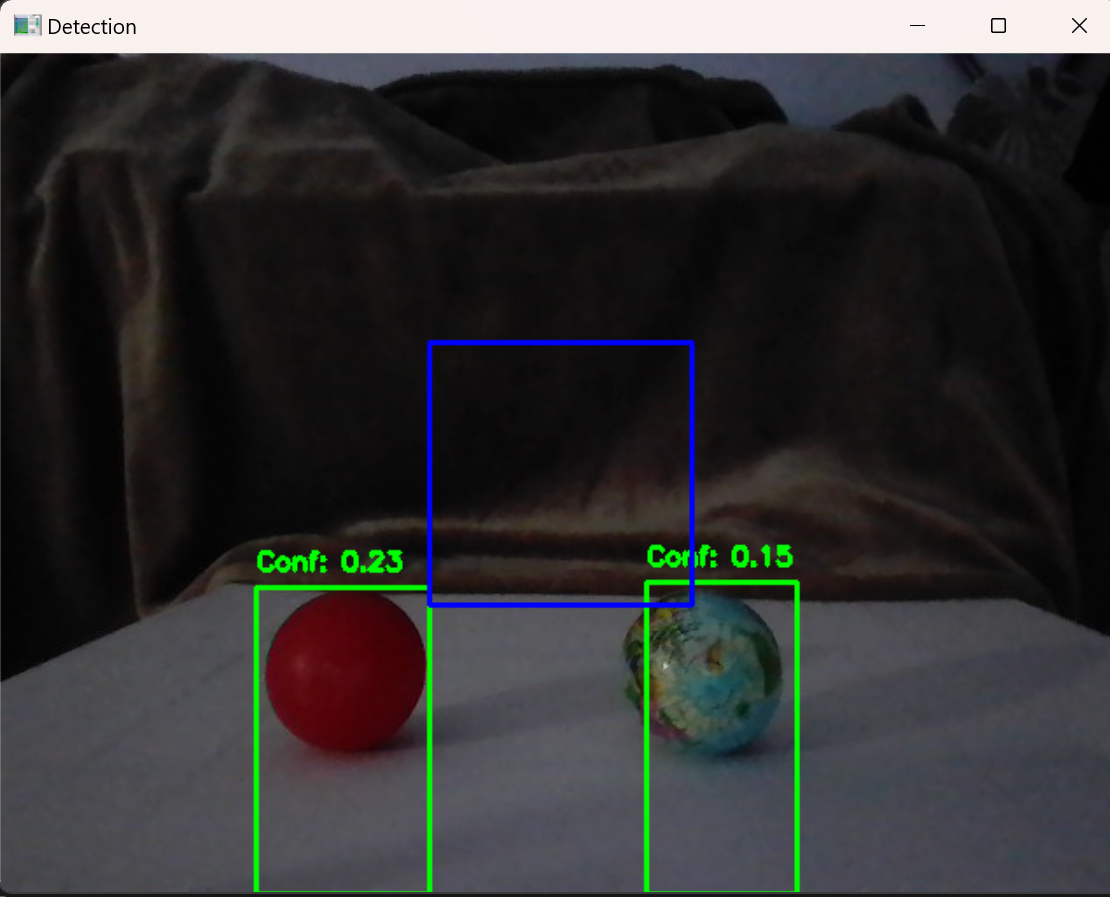
\includegraphics[width=0.5\textwidth]{Images/Porownanie/Yolo7 robot/Zrzut ekranu 2025-01-02 194208.png}
    \caption{Sytuacja przy gorszym oświetleniu — poprawne wykrycie piłki czerwonej oraz błędne wskazanie piłki o innych barwach.}
    \label{fig:Wykrycie_piłki2}
\end{figure}

\newpage
Analiza wyników wykazała, że system wizyjny działa poprawnie w warunkach dobrego oświetlenia, precyzyjnie identyfikując piłkę czerwoną oraz ignorując inne obiekty.

W przypadku słabego oświetlenia zauważono spadek skuteczności systemu. Algorytm błędnie klasyfikuje obiekt o podobnym kształcie jako piłkę, co może wynikać z niewystarczającej jakości danych treningowych dla scen o niskim poziomie światła. Mimo to system nadal rozpoznaje piłkę czerwoną, co świadczy o jego częściowej odporności na zmienne warunki oświetleniowe.

\begin{figure}[!hb]
    \centering
    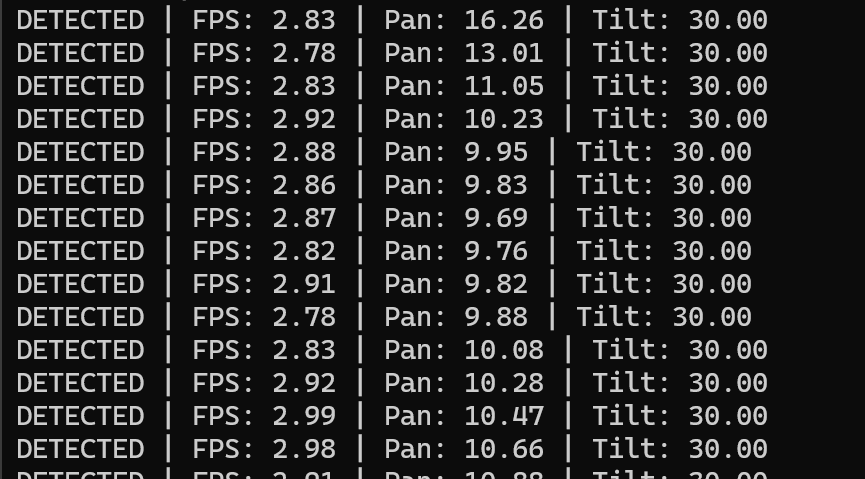
\includegraphics[width=0.6\textwidth]{Images/Porownanie/Yolo7 robot/Para pilek ciemno poprawnie wskazal czerwona.png}
    \caption{Informacja zwrotna w terminalu Raspberry Pi o wykryciu piłki czerwonej}
    \label{fig:TerminalOutput}
\end{figure}

\textbf{Rysunek}~\ref{fig:TerminalOutput} przedstawia widok terminala programu uruchomionego na Raspberry Pi. Jest to widok sytuacji, w której otoczenie jest dobrze oświetlone a program poprawnie wskazał czerwoną piłkę. W sytuacji gorszego oświetlenia i błędnej detekcji dwóch obiektów, program utrzymuje współrzędne serwomechanizmów dla pierwszego zidentyfikowanego obiektu. Ze względu na ograniczone zasoby mocy obliczeniowej Raspberry Pi, zdecydowano się na rezygnację z wyświetlania obrazu bezpośrednio na urządzeniu. Informacje o detekcji, takie jak status wykrycia obiektu \textbf{DETECTED} (oznaczające "Wykryto") oraz \textbf{SEARCHING} (oznaczające "Szukanie"), wartości kątów serwomechanizmów \textbf{Pan} (oznaczający "Obrót" wokół osi pionowej) i \textbf{Tilt} (oznaczający "Przechył" wokół osi pionowej) oraz liczba klatek na sekundę (\textbf{FPS}), są przesyłane do terminala komputera połączonego z Raspberry Pi przez SSH.

Warto zauważyć, że \textbf{Rysunki}~\ref{fig:Wykrycie_piłki1} i~\ref{fig:Wykrycie_piłki2} ilustrują działanie tego samego programu, lecz uruchomionego na komputerze w celu wizualizacji. Na obrazach widoczny jest niebieski kwadrat w centrum kadru, który wyznacza obszar uznawany za środek obrazu. Dzięki jego zastosowaniu program jest w stanie bardziej stabilnie śledzić pozycję obiektu. 



\newpage
W celu oceny skuteczności zaprojektowanego systemu wizyjnego przeprowadzono testy w różnych warunkach oświetleniowych oraz w obecności obiektów potencjalnie zakłócających detekcję piłki. Analiza wyników opierała się na obserwacji działania programu w scenariuszach symulujących rzeczywiste sytuacje. Na \textbf{Rysunku} \ref{fig:Wykrycie piłki3} przedstawiono sytuację, w której system działał w warunkach dobrego oświetlenia. Detekcja piłki czerwonej została przeprowadzona prawidłowo, a inne obiekty, takie jak czerwona poduszka znajdująca się w kadrze, zostały skutecznie zignorowane. Wynik ten potwierdza, że mechanizm filtrowania wyników detekcji, oparty na \textit{non-max suppression}, skutecznie eliminuje zbędne ramki detekcji.

\textbf{Rysunek} \ref{fig:Wykrycie piłki4} prezentuje wyniki systemu w trudniejszych warunkach oświetleniowych, w których detekcja piłki czerwonej została przeprowadzona poprawnie, mimo ograniczonej widoczności. Co więcej, system zignorował obiekt o zbliżonym kolorze (czerwoną poduszkę), co świadczy o zdolności modelu do rozróżniania kluczowych cech obiektów.

\begin{figure}[!hb]
    \centering
    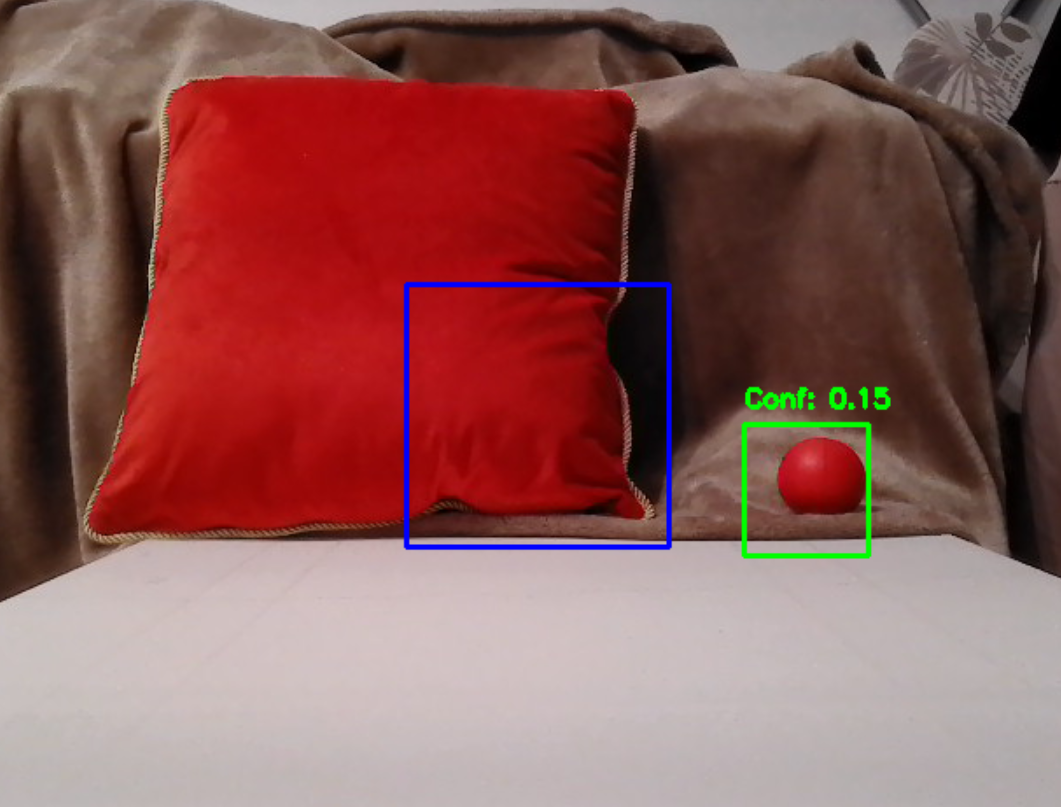
\includegraphics[width=0.5\textwidth]{Images/Porownanie/Yolo7 robot/Zrzut ekranu 2025-01-02 194354.png}
    \caption{Sytuacja przy dobrym oświetleniu - poprawne wykrycie piłki czerwonej oraz zignorowanie czerwonego obiektu.}
    \label{fig:Wykrycie piłki3}
\end{figure}

\begin{figure}[!hb]
    \centering
    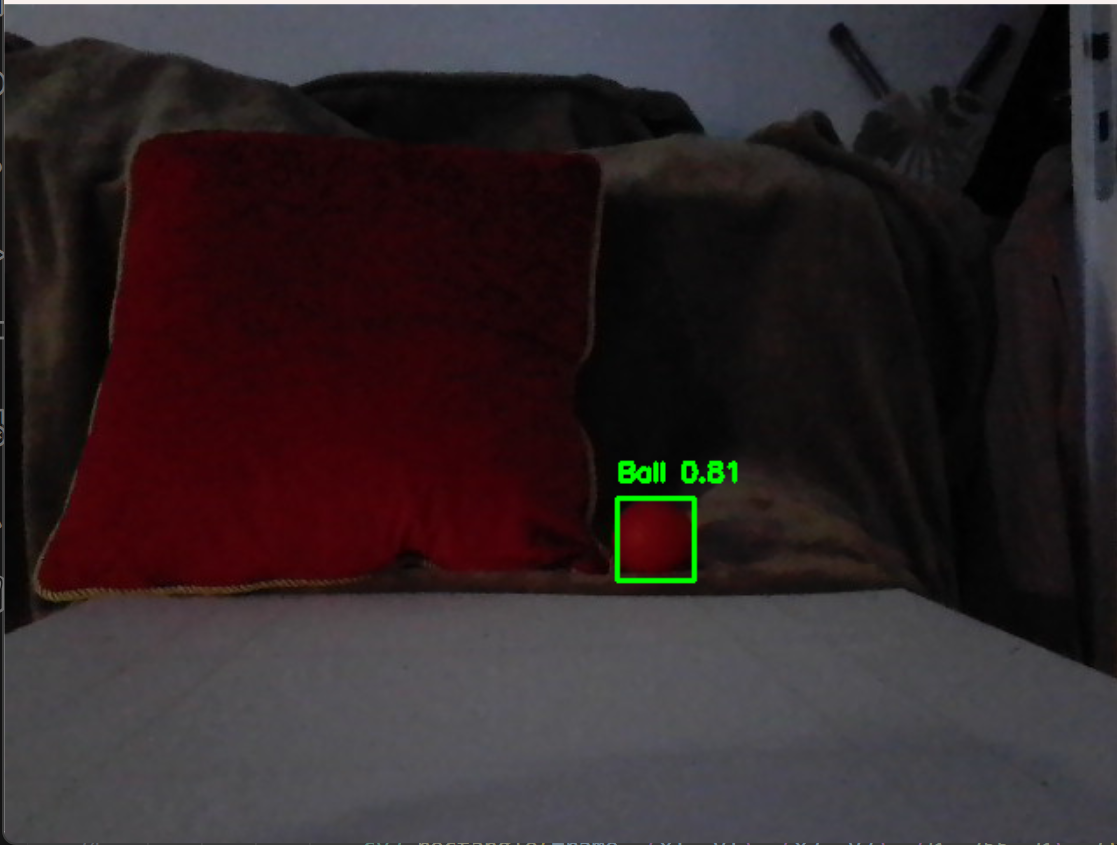
\includegraphics[width=0.5\textwidth]{Images/Porownanie/Yolo7 robot/Zrzut ekranu 2025-01-02 194641.png}
    \caption{Sytuacja przy złym oświetleniu - poprawne wykrycie piłki czerwonej oraz poprawne zignorowanie czerwonego obiektu.}
    \label{fig:Wykrycie piłki4}
\end{figure}


\begin{figure}[h]
    \centering
    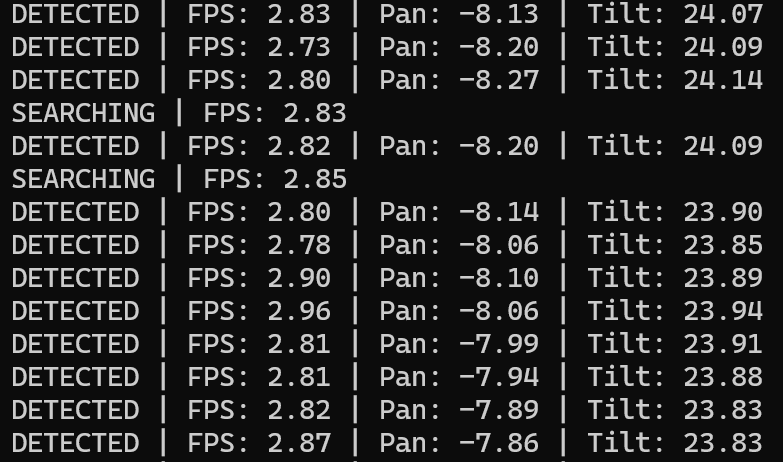
\includegraphics[width=0.6\textwidth]{Images/Porownanie/Yolo7 robot/pilka i poduszka zgaszone swiatlo dalej wykrywa.png}
    \caption{Informacja zwrotna w terminalu Raspberry Pi o wykryciu piłki czerwonej i zignorowaniu czerwonego obiektu}
    \label{fig:Wykrycie piłki5}
\end{figure}

\textbf{Rysunek} \ref{fig:Wykrycie piłki5} przedstawia widok terminala programu uruchomionego na Raspberry Pi. Jest to widok sytuacji, w której otoczenie jest dobrze oświetlone a program poprawnie wskazał czerwoną piłkę. Jednakże można zauważyć, iż program w pewnych momentach działania nie wykrywał modelu wcale i rozpoczął sekwencję poszukiwania. 

\newpage

\section{Detekcja obiektu za pomocą binaryzacji i klasycznych technik przetwarzania obrazów}

W podrozdziale tym przedstawiono podejście do detekcji obiektu (piłki czerwonej) z wykorzystaniem klasycznych technik przetwarzania obrazów, takich jak binaryzacja i analiza konturów. W przeciwieństwie do metod opartych na zaawansowanych modelach uczenia maszynowego, zastosowane rozwiązanie opiera się na transformacjach kolorystycznych i filtracji, co pozwala na efektywną detekcję przy ograniczonych zasobach obliczeniowych dostępnych na platformie Raspberry Pi.

\subsection{Opis działania programu}

Program rozpoczyna swoje działanie od pobrania obrazu z kamery w czasie rzeczywistym, który następnie jest przetwarzany w celu wykrycia czerwonej piłki. Proces ten opiera się na kilku kluczowych krokach:

\paragraph{Konwersja przestrzeni barw}
Pierwszym krokiem jest konwersja obrazu z przestrzeni barw RGB na przestrzeń HSV (ang. \textit{Hue, Saturation, Value}). Przestrzeń HSV umożliwia łatwiejszą separację kolorów, co jest szczególnie przydatne przy detekcji obiektów o specyficznej barwie. Konwersję realizuje funkcja \texttt{cv2.cvtColor}, której działanie przedstawiono w Kodzie~\ref{lst:hsv_conversion}.

\begin{lstlisting}[language=Python, caption={Konwersja obrazu z przestrzeni RGB do HSV.}, label={lst:hsv_conversion}, captionpos=b]
hsv = cv2.cvtColor(frame, cv2.COLOR_BGR2HSV)
\end{lstlisting}

\paragraph{Binaryzacja obrazu}
W celu wyodrębnienia obszarów odpowiadających kolorowi czerwonej piłki zastosowano binaryzację z użyciem dwóch zakresów wartości HSV. Zakresy te uwzględniają różne odcienie czerwieni występujące w przestrzeni barw HSV, co pozwala na dokładniejsze uchwycenie piłki. Fragment kodu odpowiedzialny za binaryzację przedstawiono w Kodzie~\ref{lst:binaryzation}.

\begin{lstlisting}[language=Python, caption={Binaryzacja obrazu w oparciu o zakresy HSV.}, label={lst:binaryzation}, captionpos=b]
lower_red1 = np.array([0, 120, 70])
upper_red1 = np.array([10, 255, 255])
lower_red2 = np.array([170, 120, 70])
upper_red2 = np.array([180, 255, 255])

mask1 = cv2.inRange(hsv, lower_red1, upper_red1)
mask2 = cv2.inRange(hsv, lower_red2, upper_red2)
mask = cv2.add(mask1, mask2)
\end{lstlisting}

Binaryzacja generuje maskę, w której piksele należące do zakresów koloru czerwonego mają wartość 1, a pozostałe - 0. Dzięki połączeniu dwóch zakresów (dolnego i górnego), algorytm uwzględnia różnice w odcieniach czerwieni, które mogą występować w różnych warunkach oświetleniowych.

\paragraph{Analiza konturów}
Na kolejnym etapie program identyfikuje kontury obiektów na binaryzowanej masce. Dla każdego z konturów obliczana jest powierzchnia oraz okrągłość, która pozwala odrzucić obiekty o kształtach znacząco różniących się od idealnego okręgu. Kryterium okrągłości obiektu opiera się na stosunku powierzchni konturu do pola powierzchni okręgu opisanego na konturze. Kod odpowiedzialny za analizę konturów przedstawiono w Kodzie~\ref{lst:contour_analysis}.

\begin{lstlisting}[language=Python, caption={Analiza konturów w celu identyfikacji piłki.}, label={lst:contour_analysis}, captionpos=b]
contours, _ = cv2.findContours(mask, cv2.RETR_EXTERNAL, cv2.CHAIN_APPROX_SIMPLE)

for contour in contours:
    area = cv2.contourArea(contour)
    if area > 300:
        ((x, y), radius) = cv2.minEnclosingCircle(contour)
        circle_area = np.pi * (radius ** 2)
        if 0.6 < area / circle_area < 1.4:
            ball_center_x = int(x)
            ball_center_y = int(y)
            detected = True
\end{lstlisting}

\newpage
\subsection{Uzyskane rezultaty}
Wyniki działania algorytmu detekcji obiektu za pomocą binaryzacji zostały przedstawione w formie dwóch widoków dla każdego przypadku testowego. Pierwszy widok przedstawia obraz po zastosowaniu binaryzacji, gdzie piksele odpowiadające wykrytej barwie zostały zaznaczone na biało, a pozostałe wykluczone. Drugi widok prezentuje obraz w przestrzeni barw HSV, co umożliwia wizualną ocenę zakresów kolorów zastosowanych w procesie binaryzacji. Należy zaznaczyć, że wizualizacja ta została uruchomiona na komputerze, podczas gdy na Raspberry Pi wyświetlana jest jedynie informacja w terminalu o wykryciu bądź braku wykrycia obiektu.

Na \textbf{Rysunku}~\ref{fig:Wykrycie piłki6} zaprezentowano przykład wykrycia czerwonej piłki w dalekim kadrze przy słabym oświetleniu. Algorytm prawidłowo zidentyfikował piłkę, co dowodzi jego zdolności do poprawnej detekcji w trudnych warunkach oświetleniowych. Podobny przypadek przedstawiono na \textbf{Rysunku}~\ref{fig:Wykrycie piłki7}, gdzie piłka została prawidłowo wykryta w dobrych warunkach oświetleniowych.

\begin{figure}[h]
    \centering
    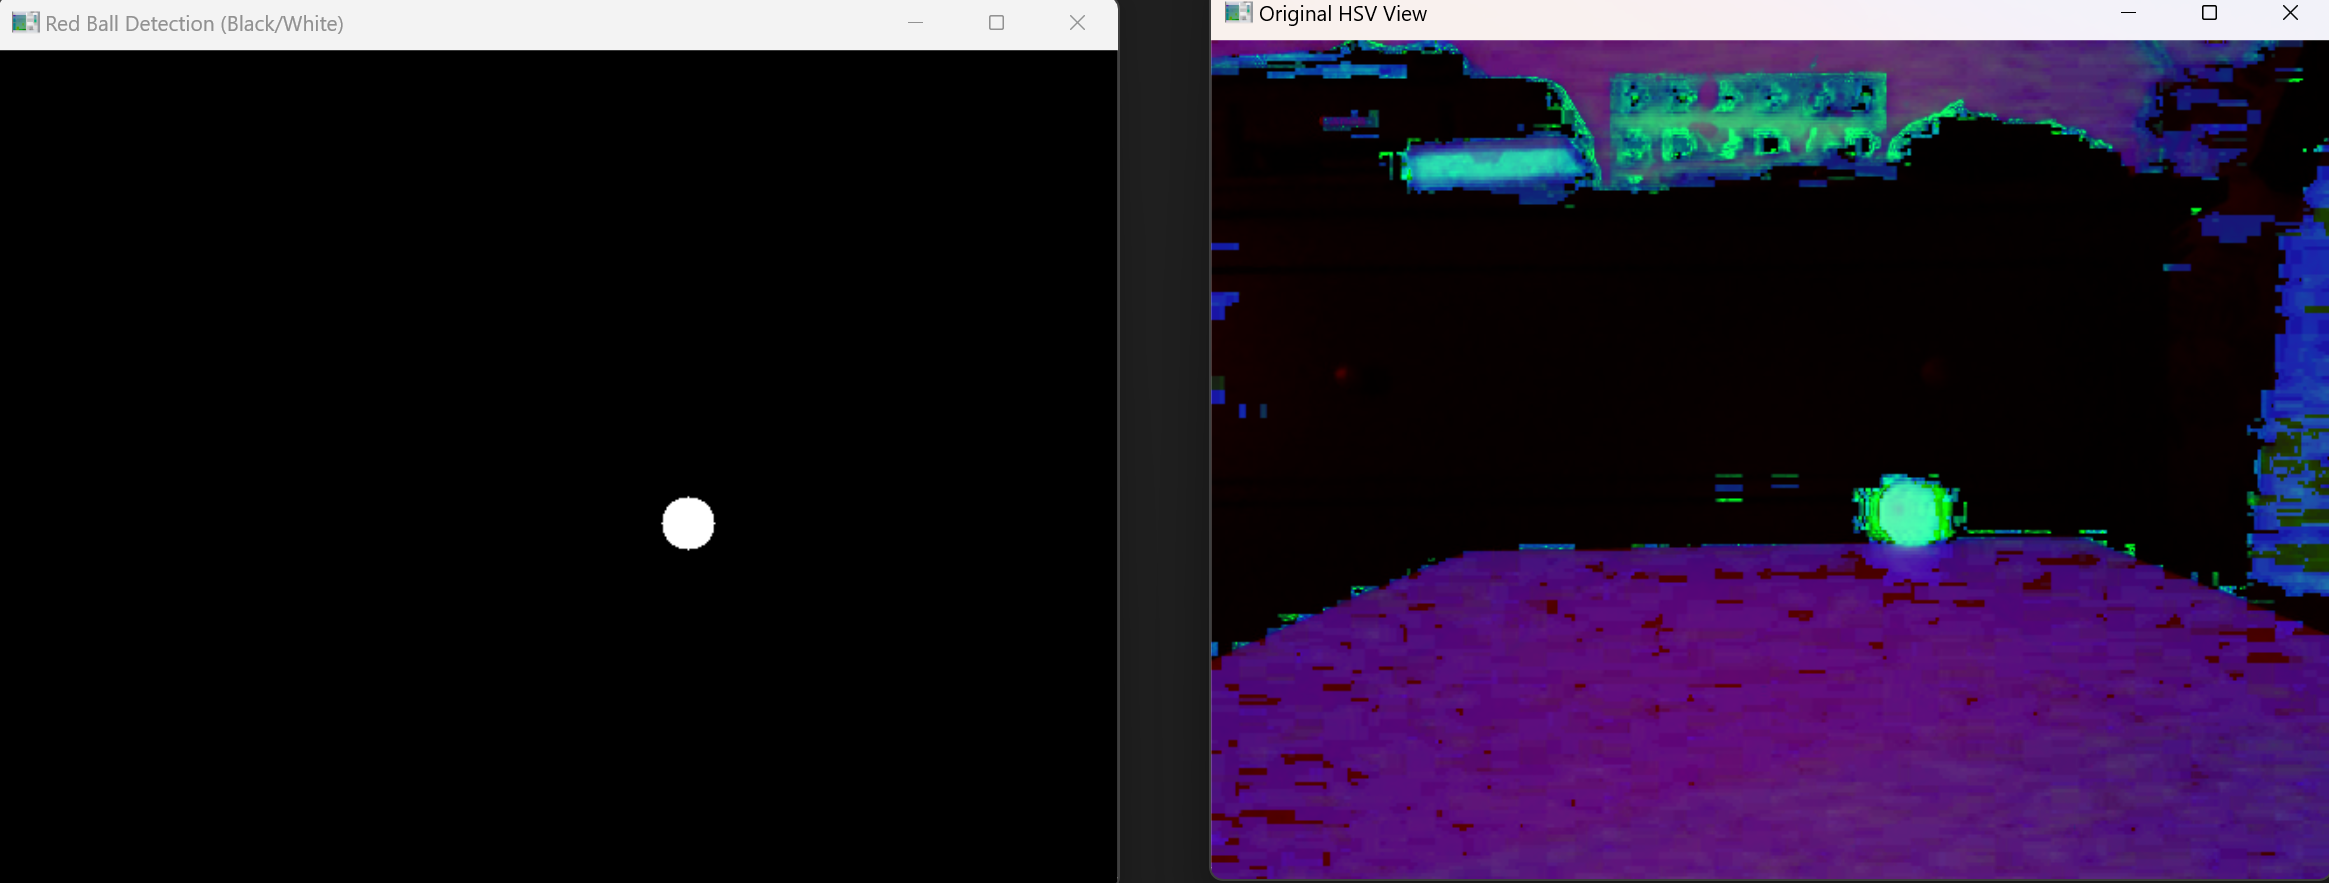
\includegraphics[width=0.9\textwidth]{Images/Porownanie/Binaryzacja/Zrzut ekranu 2025-01-02 193719.png}
    \caption{Sytuacja przy złym oświetleniu - poprawne wykrycie czerwonej piłki w dalekim kadrze}
    \label{fig:Wykrycie piłki6}
\end{figure}
\begin{figure}[h]
    \centering
    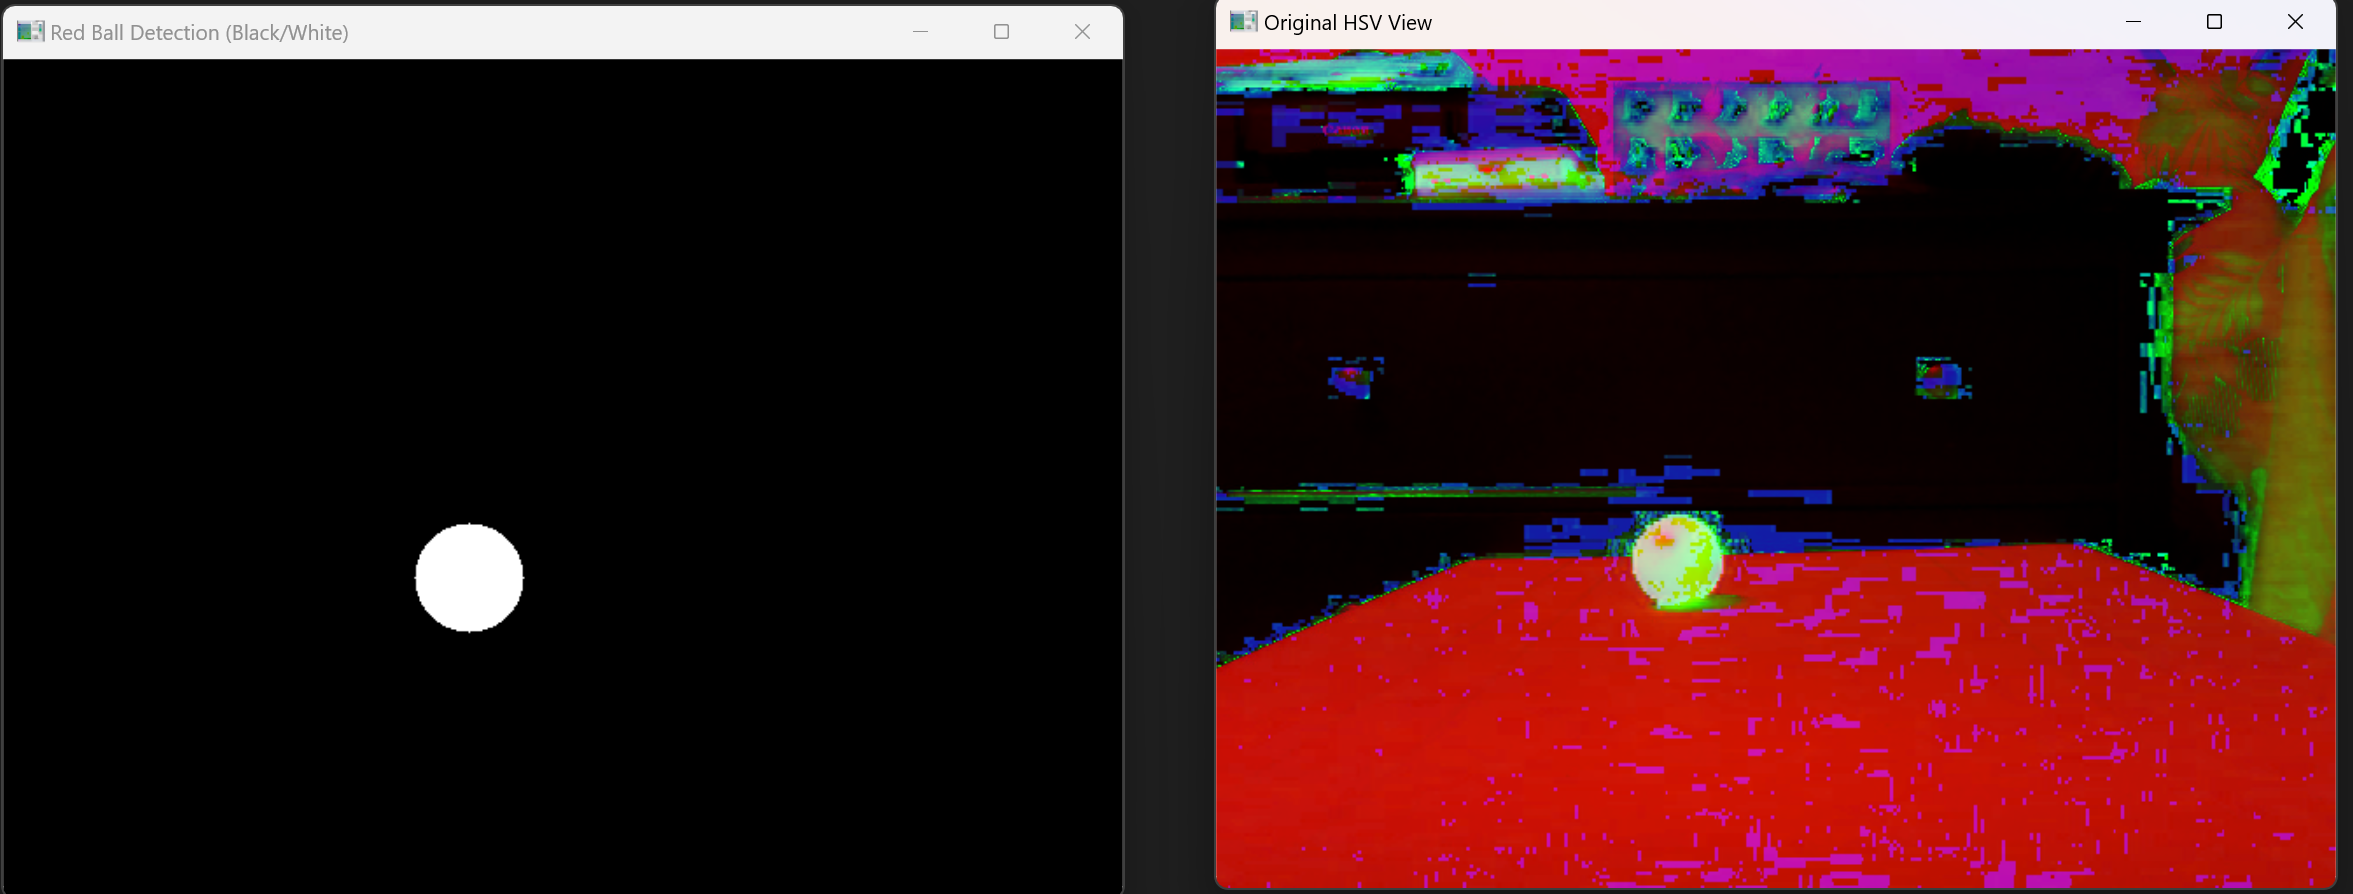
\includegraphics[width=0.9\textwidth]{Images/Porownanie/Binaryzacja/Zrzut ekranu 2025-01-02 193549.png}
    \caption{Sytuacja przy dobrym oświetleniu - poprawne wykrycie czerwonej piłki w dalekim kadrze}
    \label{fig:Wykrycie piłki7}
\end{figure}

Należy również zauważyć, że podczas działania algorytmu na Raspberry Pi skuteczność detekcji była bardziej wrażliwa na warunki oświetleniowe. W momencie, gdy natężenie światła uległo znacznemu zmniejszeniu, program przestał wykrywać czerwoną piłkę. Na obrazie przedstawionym na \textbf{Rysunku}~\ref{fig:Wykrycie piłki Rasp} widoczny jest moment, w którym światło zostało zgaszone, co spowodowało przejście informacji w terminalu z \textbf{DETECTED} na \textbf{SEARCHING}.


Zjawisko to wskazuje na ograniczenia algorytmu wynikające z braku wystarczającej ilości informacji w warunkach słabego oświetlenia. Raspberry Pi, mimo zastosowania prostych i wydajnych metod takich jak binaryzacja, wykazuje ograniczenia w detekcji obiektów w trudnych warunkach oświetleniowych. Utrata detekcji w takich sytuacjach wynika głównie z ograniczeń samej metody binaryzacji, która opiera się wyłącznie na analizie kolorów, a nie z braku wystarczających zasobów obliczeniowych.
\begin{figure}[h]
    \centering
    \includegraphics[width=0.7\textwidth]{Images/Porownanie/Binaryzacja/Para piłek moment zgaszenia swiatla.png}
    \caption{Informacja zwrotna w  terminalu Raspberry Pi - zgubienie piłki w momencie zgaszenia światła}
    \label{fig:Wykrycie piłki Rasp}
\end{figure}


\newpage

\textbf{Rysunki}~\ref{fig:Wykrycie piłki8} i~\ref{fig:Wykrycie piłki9} przedstawiają wyniki działania algorytmu w bliskim kadrze. W przypadku słabego oświetlenia (\textbf{Rysunek}~\ref{fig:Wykrycie piłki8}), algorytm poprawnie zidentyfikował piłkę oraz zignorował inny obiekt o podobnym kolorze. Natomiast w lepszych warunkach oświetleniowych (\textbf{Rysunek}~\ref{fig:Wykrycie piłki9}) zarejestrowano błędne wskazanie czerwonego obiektu znajdującego się w tle. Wynik ten wskazuje, że intensywne oświetlenie może zwiększyć prawdopodobieństwo fałszywych detekcji.

\begin{figure}[h]
    \centering
    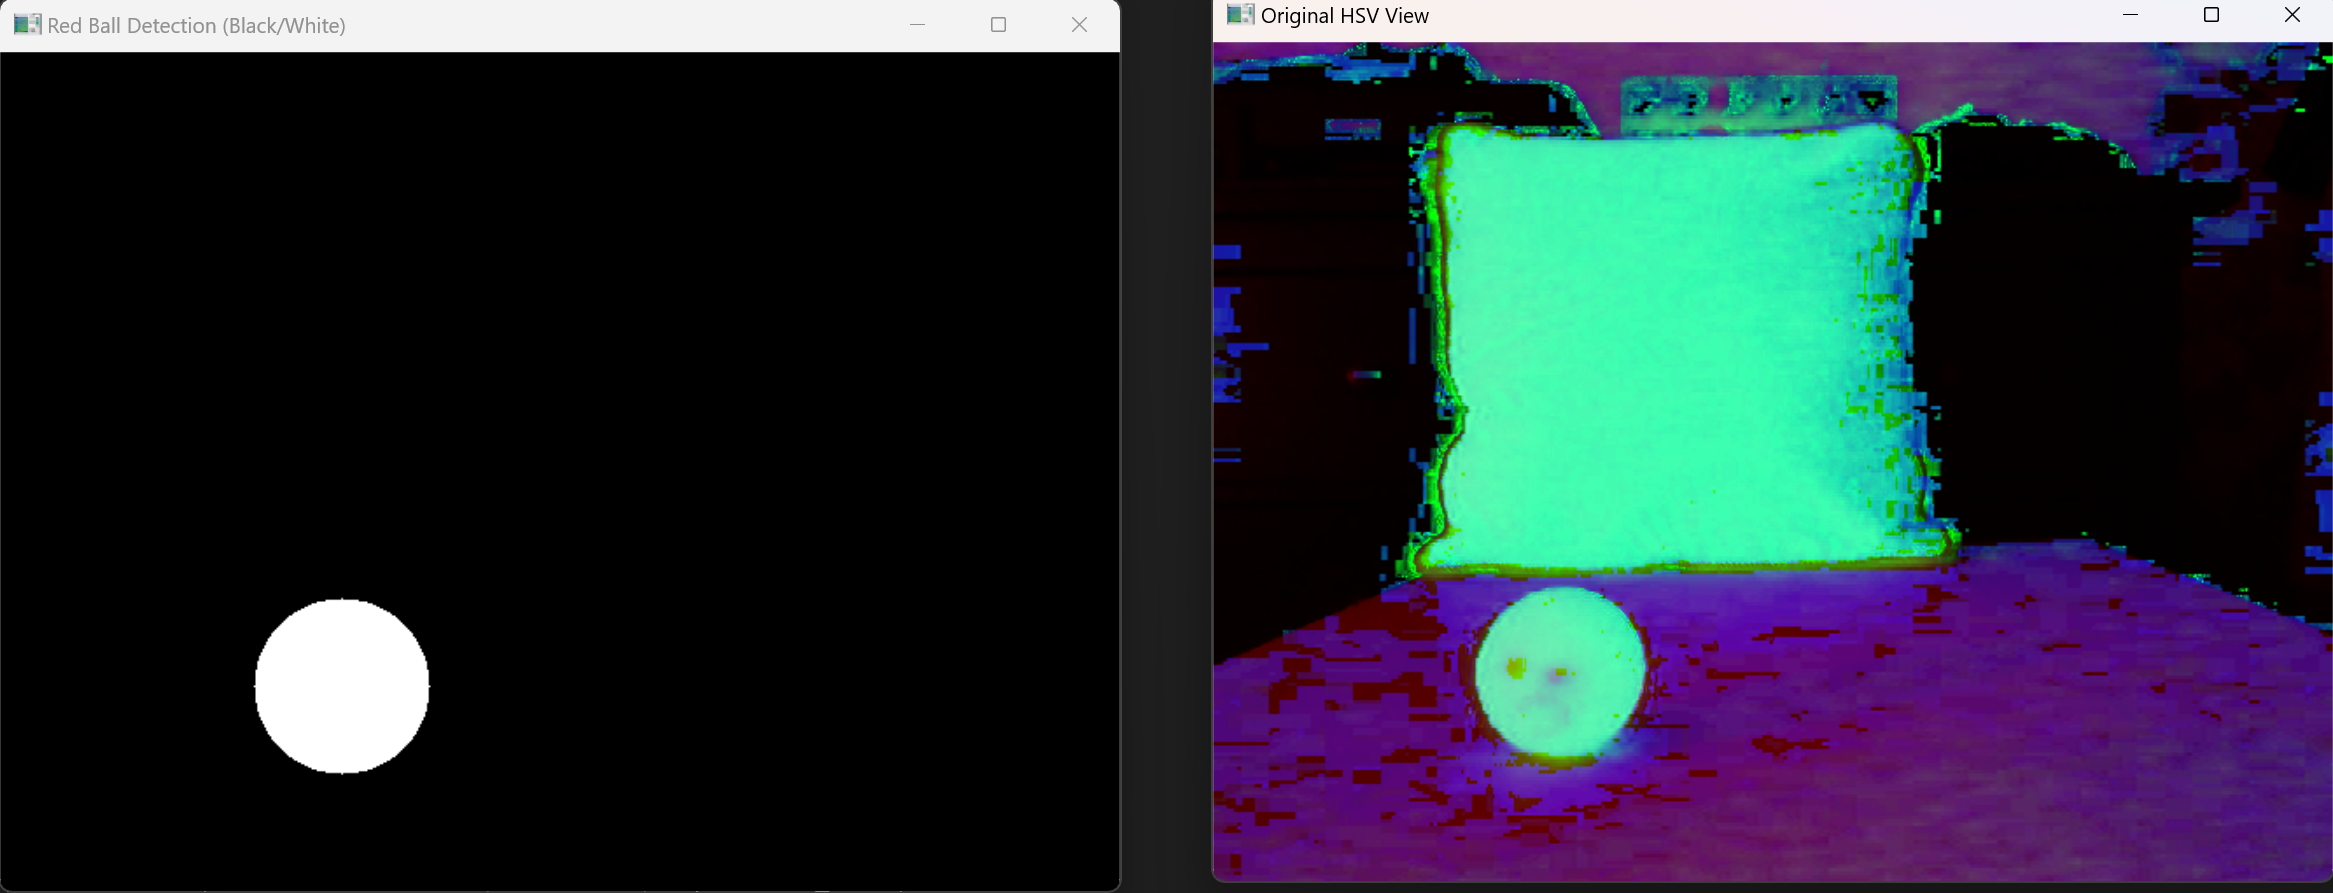
\includegraphics[width=0.9\textwidth]{Images/Porownanie/Binaryzacja/Zrzut ekranu 2025-01-02 193840.png}
    \caption{Sytuacja przy złym oświetleniu - poprawne wykrycie czerwonej piłki w bliskim kadrze oraz zignorowanie czerwonego obiektu}
    \label{fig:Wykrycie piłki8}
\end{figure}

\begin{figure}[h]
    \centering
    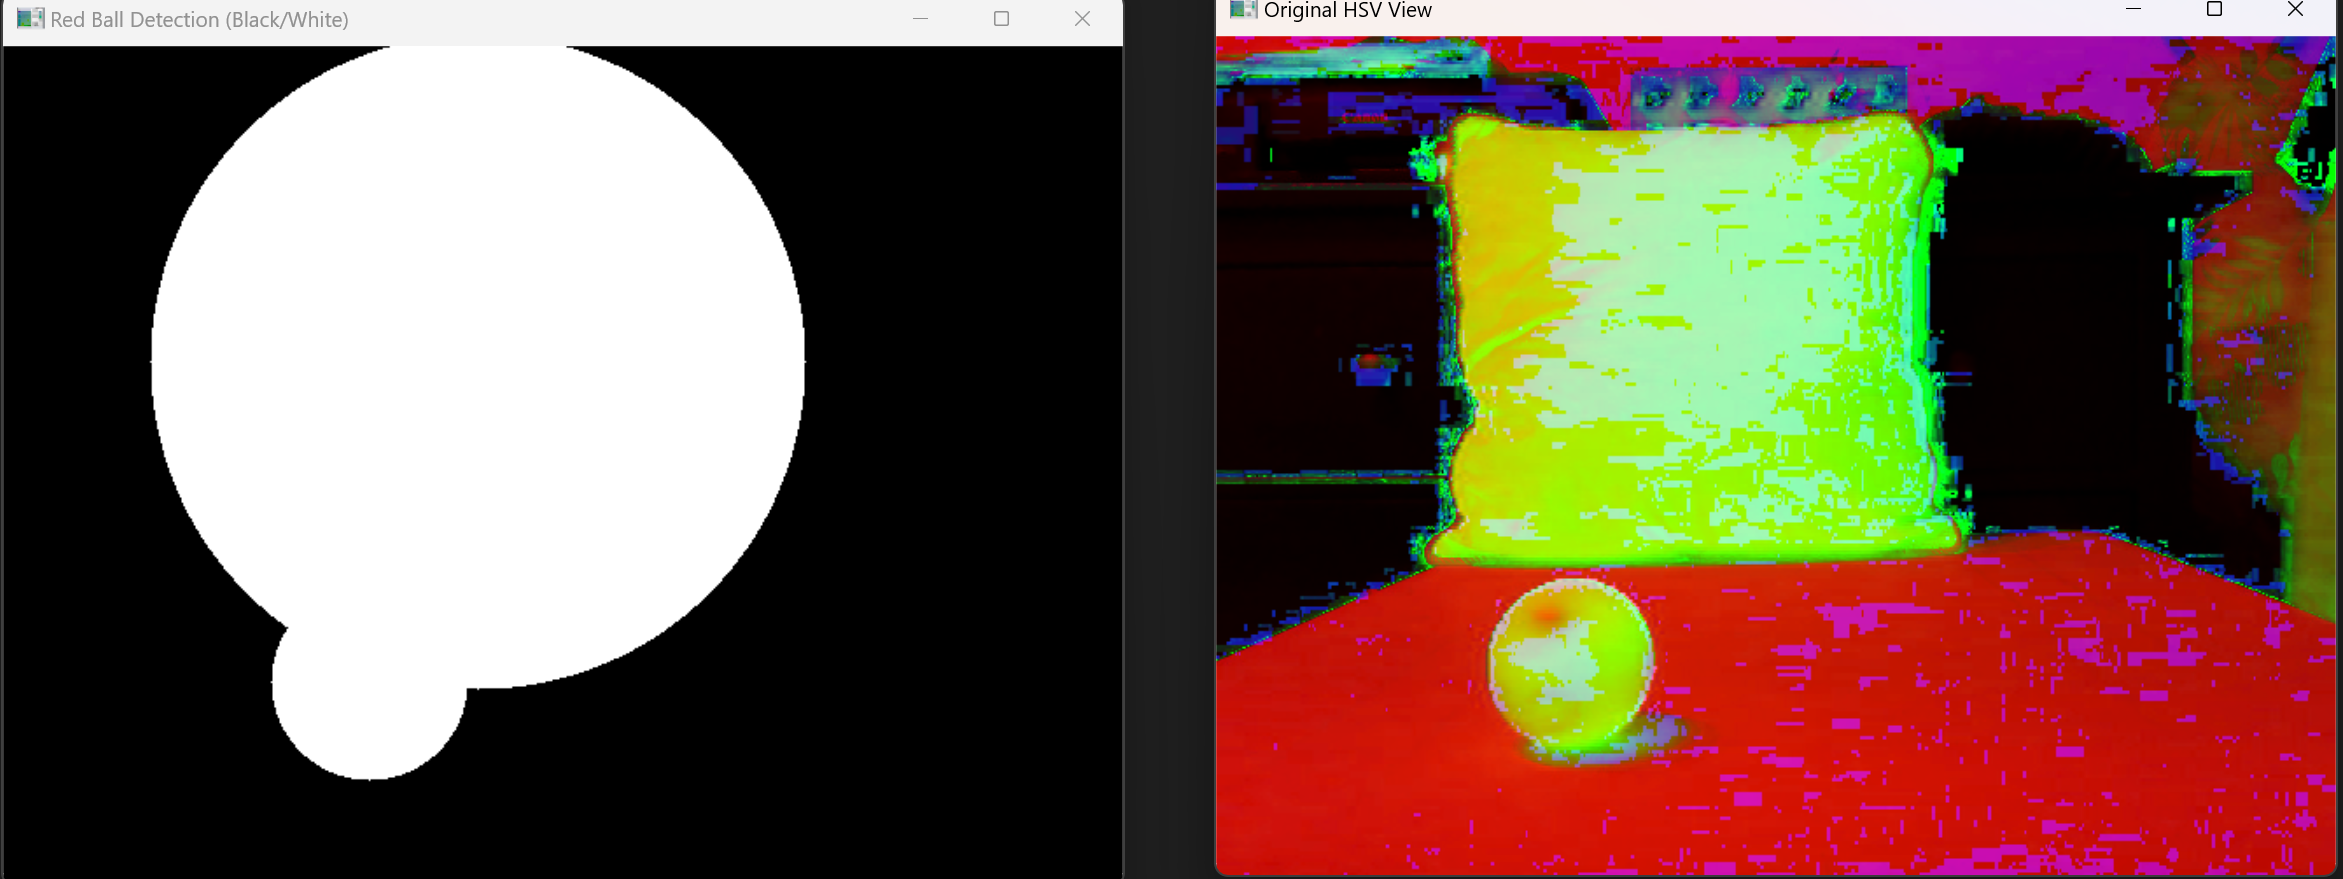
\includegraphics[width=0.9\textwidth]{Images/Porownanie/Binaryzacja/Zrzut ekranu 2025-01-02 193858.png}
    \caption{Sytuacja przy dobrym oświetleniu - poprawne wykrycie czerwonej piłki oraz błędne wskazanie czerwonego obiektu}
    \label{fig:Wykrycie piłki9}
\end{figure}

\newpage

Kolejny test, zilustrowany na \textbf{Rysunku}~\ref{fig:Wykrycie piłki10}, pokazuje odporność algorytmu na zakłócenia w gorszych warunkach oświetleniowych. W warunkach ograniczonego oświetlenia algorytm poprawnie ignorował czerwone obiekty inne niż piłka (\textbf{Rysunek}~\ref{fig:Wykrycie piłki10}), co dowodzi jego skuteczności w rozróżnianiu obiektów o podobnej barwie. 

Jednakże, w sytuacji przedstawionej na \textbf{Rysunku}~\ref{fig:Wykrycie piłki11}, przy dobrym oświetleniu, algorytm błędnie zidentyfikował poduszkę jako piłkę. W efekcie, rzeczywista piłka, znajdująca się na tle poduszki nie została wykryta w procesie detekcji. Ten przypadek ujawnia istotne ograniczenie algorytmu, wynikające z faktu, że analiza barwy nie jest w pełni wystarczającym kryterium identyfikacji obiektów, szczególnie w scenariuszach, gdzie różne obiekty o zbliżonym kolorze występują w tej samej scenie.

\begin{figure}[h]
    \centering
    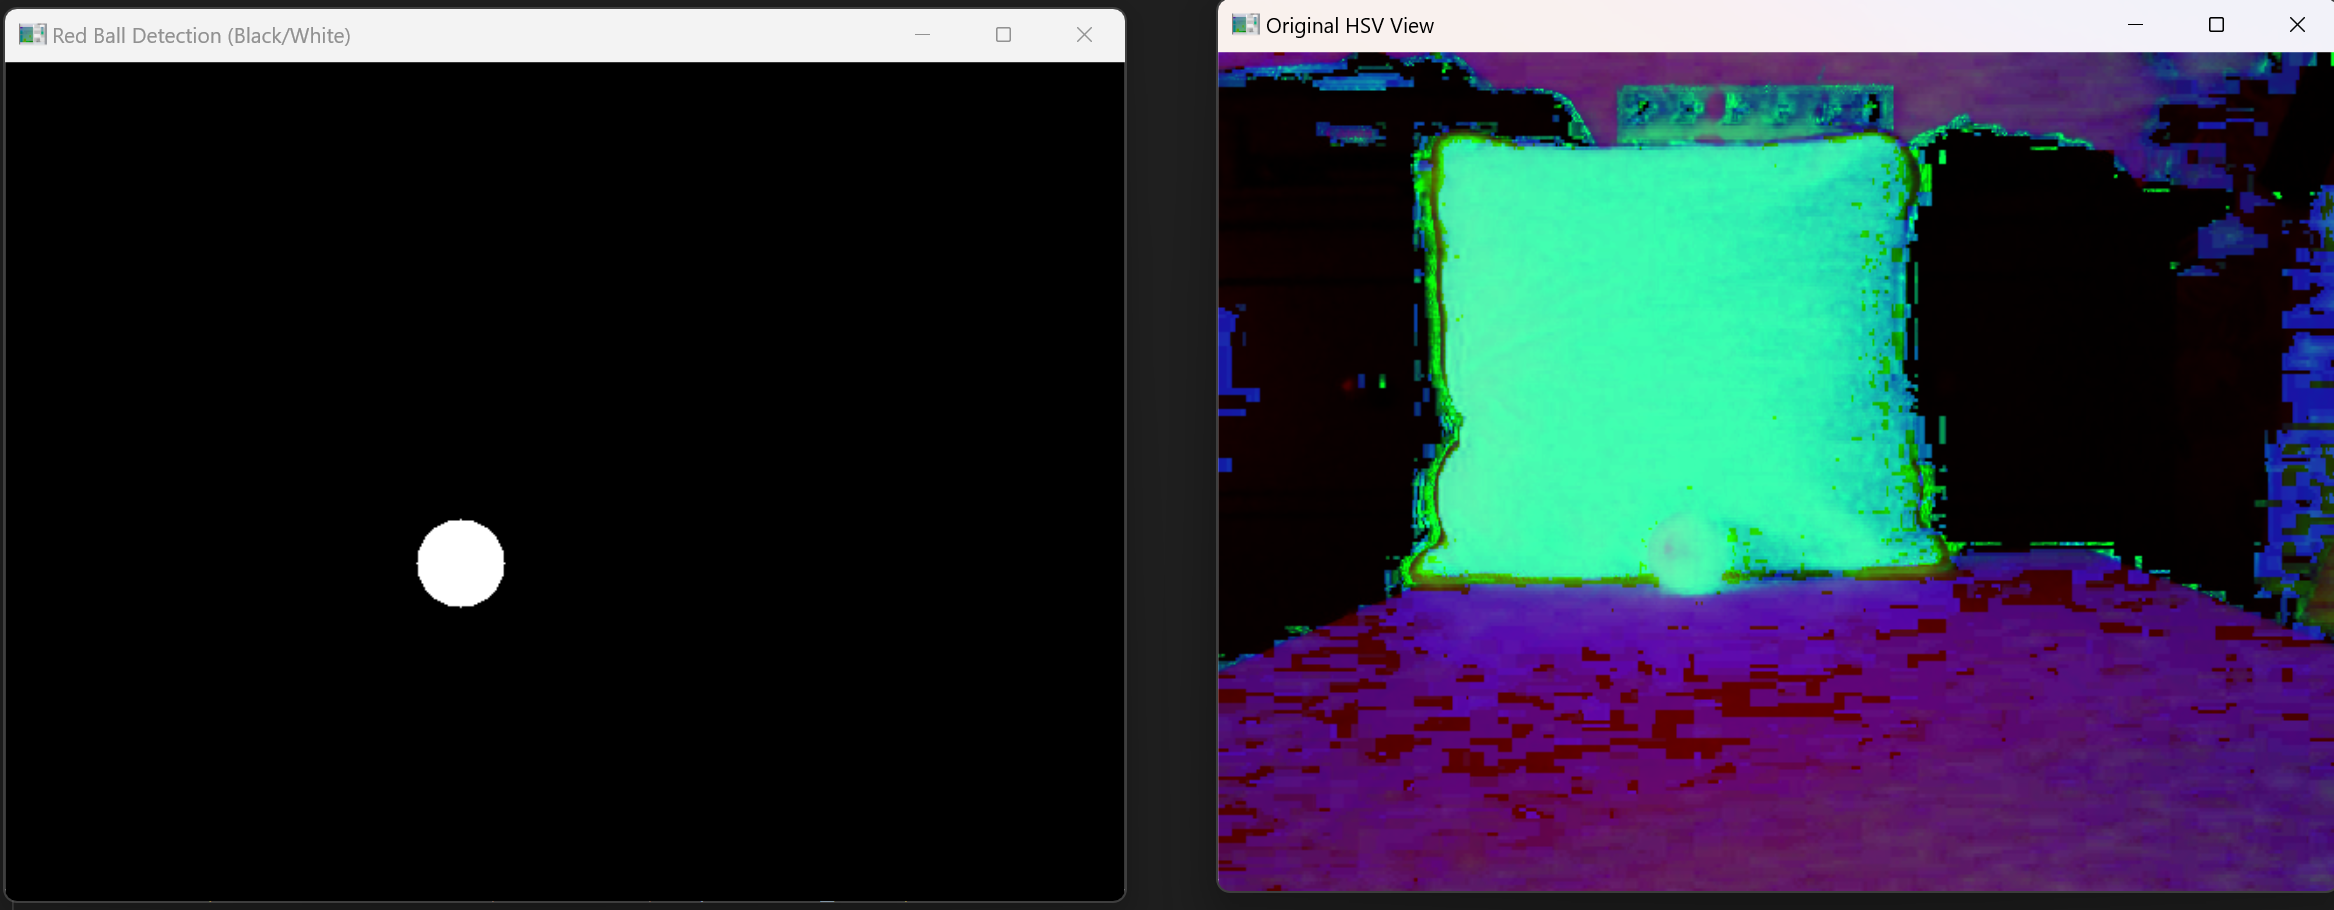
\includegraphics[width=0.9\textwidth]{Images/Porownanie/Binaryzacja/Zrzut ekranu 2025-01-02 193817.png}
    \caption{Sytuacja przy złym oświetleniu - poprawne wykrycie czerwonej piłki oraz zignorowanie czerwonego obiektu}
    \label{fig:Wykrycie piłki10}
\end{figure}
\begin{figure}[h]
    \centering
    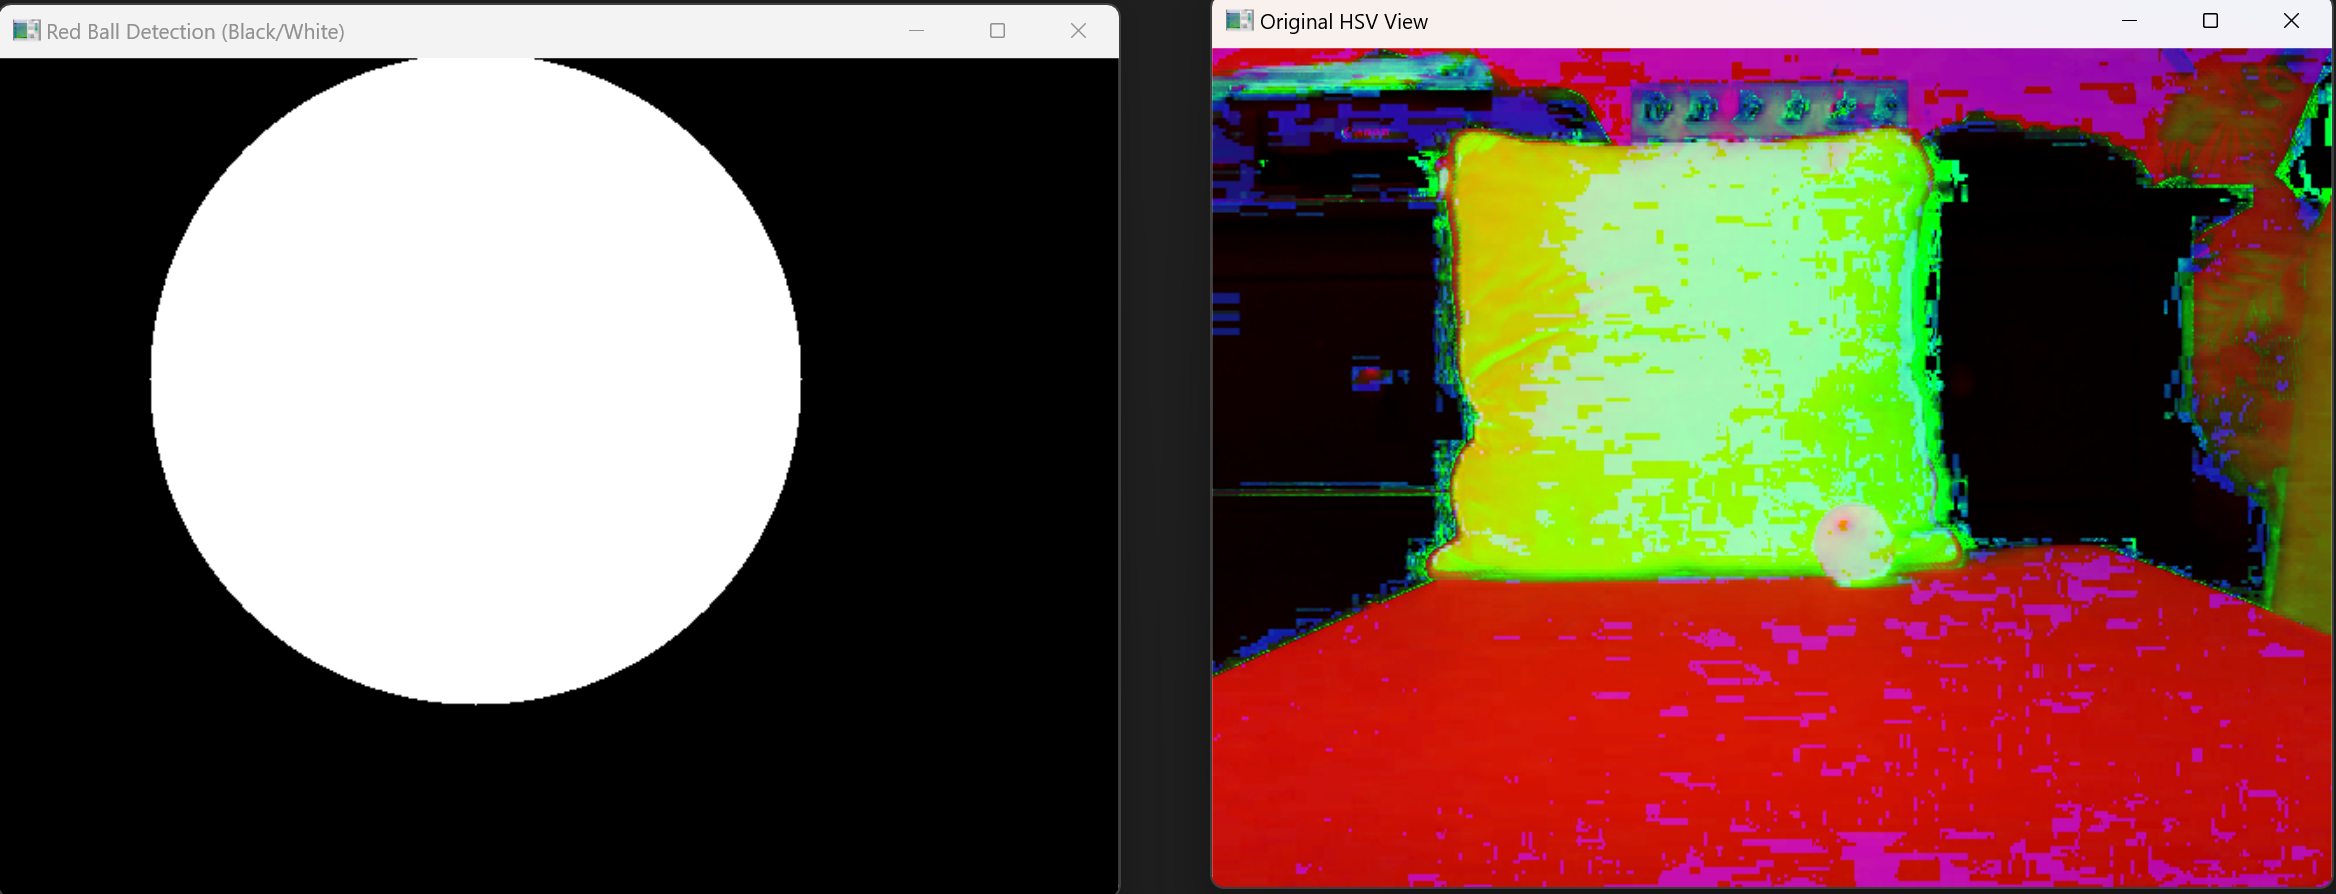
\includegraphics[width=0.9\textwidth]{Images/Porownanie/Binaryzacja/Zrzut ekranu 2025-01-02 193917.png}
    \caption{Sytuacja przy dobrym oświetleniu - błędne wskazanie czerwonego obiektu zasłoniło piłkę}
    \label{fig:Wykrycie piłki11}
\end{figure}

\newpage
\section{Porównanie skuteczności algorytmów}

W niniejszym podrozdziale dokonano porównania trzech algorytmów detekcji obiektów: YOLOv7, YOLOv8 oraz algorytmu binaryzacji. Analiza została przeprowadzona w oparciu o różne warunki oświetleniowe i otoczenie, a także na dwóch platformach sprzętowych: komputerze osobistym oraz Raspberry Pi. Celem było określenie kompromisu pomiędzy szybkością działania, wyrażoną w klatkach na sekundę (FPS), a skutecznością w wykrywaniu obiektów oraz eliminacji błędnych detekcji.

W kontekście badania, platformy sprzętowe różniły się znacząco pod względem dostępnych zasobów obliczeniowych. Komputer osobisty, wyposażony w wydajny procesor i dedykowaną kartę graficzną, umożliwiał działanie algorytmów YOLO w czasie rzeczywistym z wysoką dokładnością. Natomiast dla Raspberry Pi stanowiło to wyzwanie.

Wyniki analizy uwzględniają różne scenariusze testowe, takie jak działanie algorytmów w warunkach dobrego i słabego oświetlenia, obecność przeszkód oraz różne konfiguracje sprzętowe. Pozwoliło to na kompleksowe porównanie skuteczności i efektywności rozważanych podejść, a także ocenę ich przydatności w systemach czasu rzeczywistego.


\newpage

\subsection{Charakterystyka modelu YOLOv7}

W warunkach dobrego oświetlenia model YOLOv7 wykazuje wysoką skuteczność w detekcji obiektów, co potwierdzają wyniki przedstawione na \textbf{Rysunku}~\ref{fig:yolov7_good_light}. Algorytm prawidłowo zidentyfikował piłkę czerwoną, jednocześnie ignorując inne obiekty znajdujące się w kadrze. Kluczowym punktem tego testu było sprawdzenie czy model jest w stanie zignorować obiekty o podobnym kształcie lub barwie do śledzonej piłki, co zostało potwierdzone tylko dla przypadku dobrego oświetlenia. Niestety w warunkach słabego oświetlenia, model YOLOv7 błędnie sklasyfikował obiekt o innej barwie jako piłkę, co przedstawiono na \textbf{Rysunku}~\ref{fig:yolov7_bad_light}.

\begin{figure}[h]
    \centering
    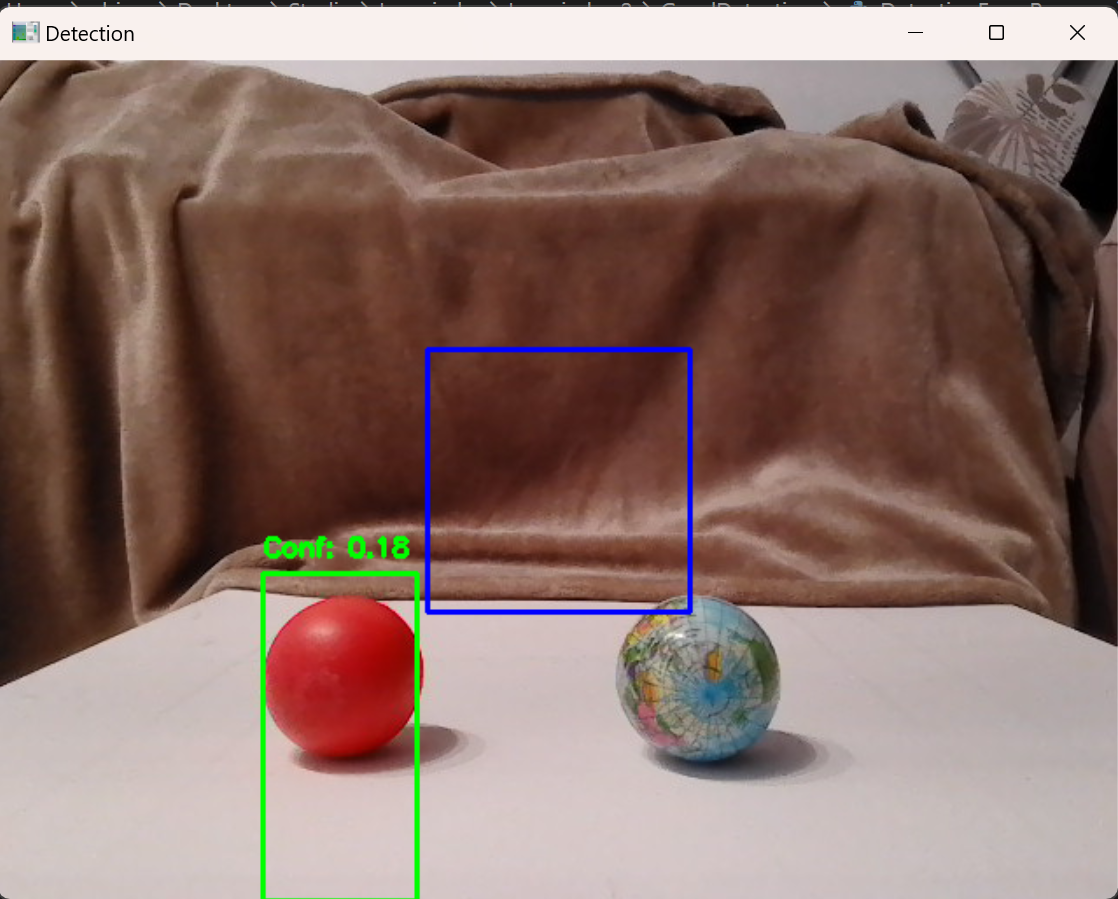
\includegraphics[width=0.6\textwidth]{Images/Porownanie/Yolo7 robot/Zrzut ekranu 2025-01-02 194147.png}
    \caption{Działanie modelu YOLOv7 przy dobrym oświetleniu.}
    \label{fig:yolov7_good_light}
\end{figure}
\begin{figure}[h]
    \centering
    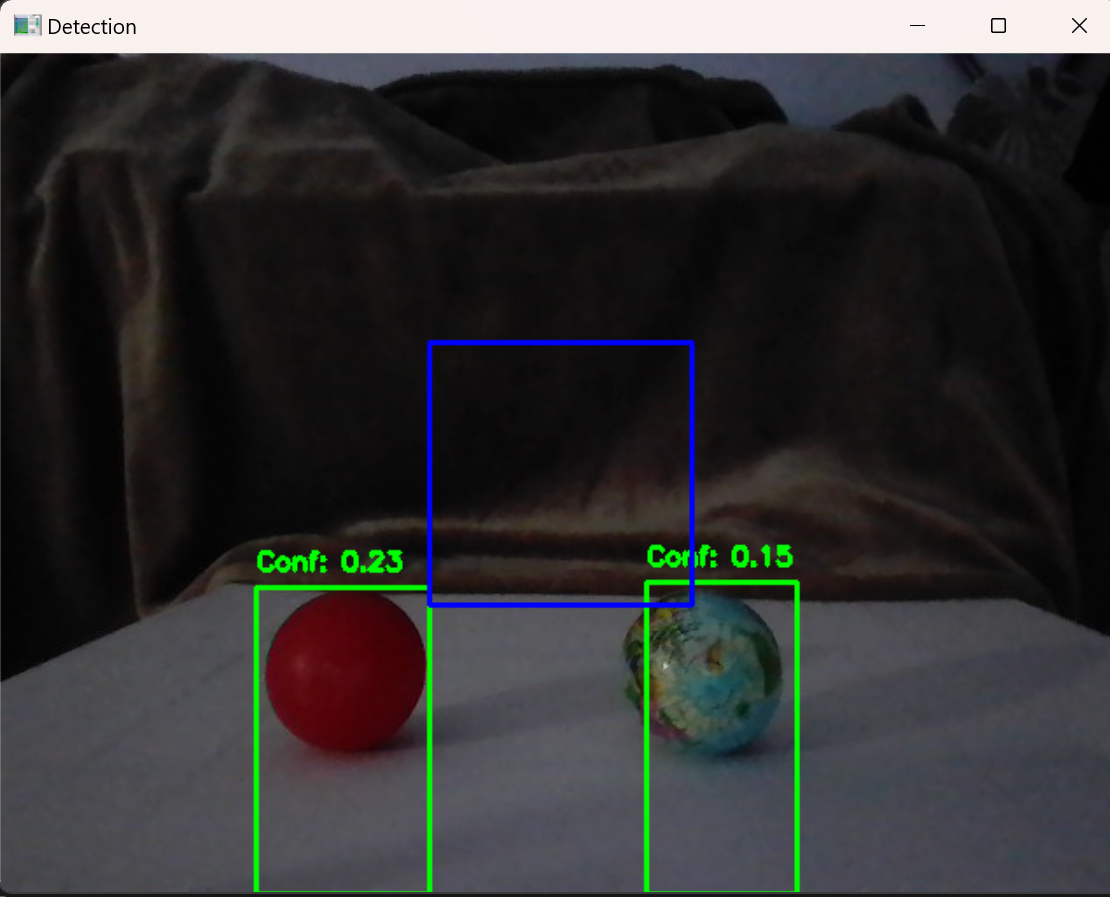
\includegraphics[width=0.6\textwidth]{Images/Porownanie/Yolo7 robot/Zrzut ekranu 2025-01-02 194208.png}
    \caption{Działanie modelu YOLOv7 przy gorszym oświetleniu.}
    \label{fig:yolov7_bad_light}
\end{figure}

\newpage
Model YOLOv7 wykazuje zdolność do prawidłowego pomijania obiektów, które nie spełniają kryteriów detekcji. Na \textbf{Rysunku}~\ref{fig:yolov7_good_light_good_object} zaprezentowano przykład działania algorytmu przy dobrym oświetleniu, gdzie obiekt w postaci czerwonej poduszki został prawidłowo pominięty. Analogicznie, w warunkach słabego oświetlenia, YOLOv7 również jest w stanie skutecznie ignorować niepożądane obiekty, co ilustruje \textbf{Rysunek}~\ref{fig:yolov7_bad_light_good_object}.

\begin{figure}[!hb]
    \centering
    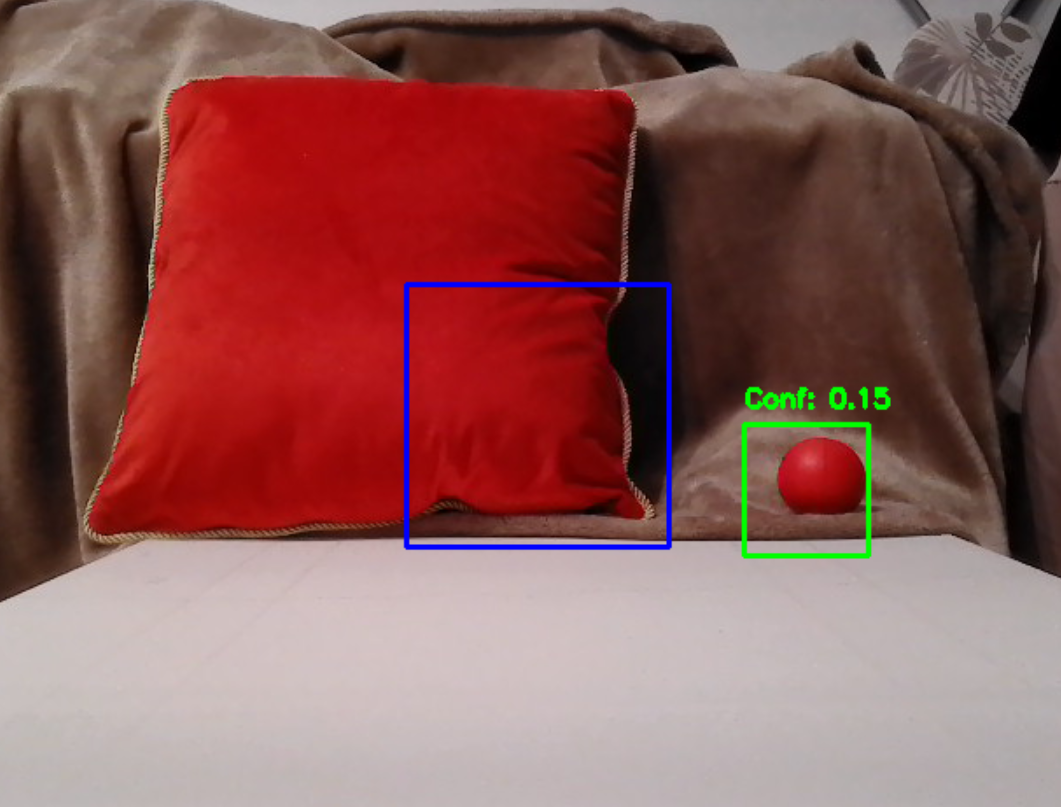
\includegraphics[width=0.6\textwidth]{Images/Porownanie/Yolo7 robot/Zrzut ekranu 2025-01-02 194354.png}
    \caption{Działanie modelu YOLOv7 przy dobrym oświetleniu - prawidłowa detekcja tylko pożądanego obiektu jakim jest piłka.}
    \label{fig:yolov7_good_light_good_object}
\end{figure}
\begin{figure}[h]
    \centering
    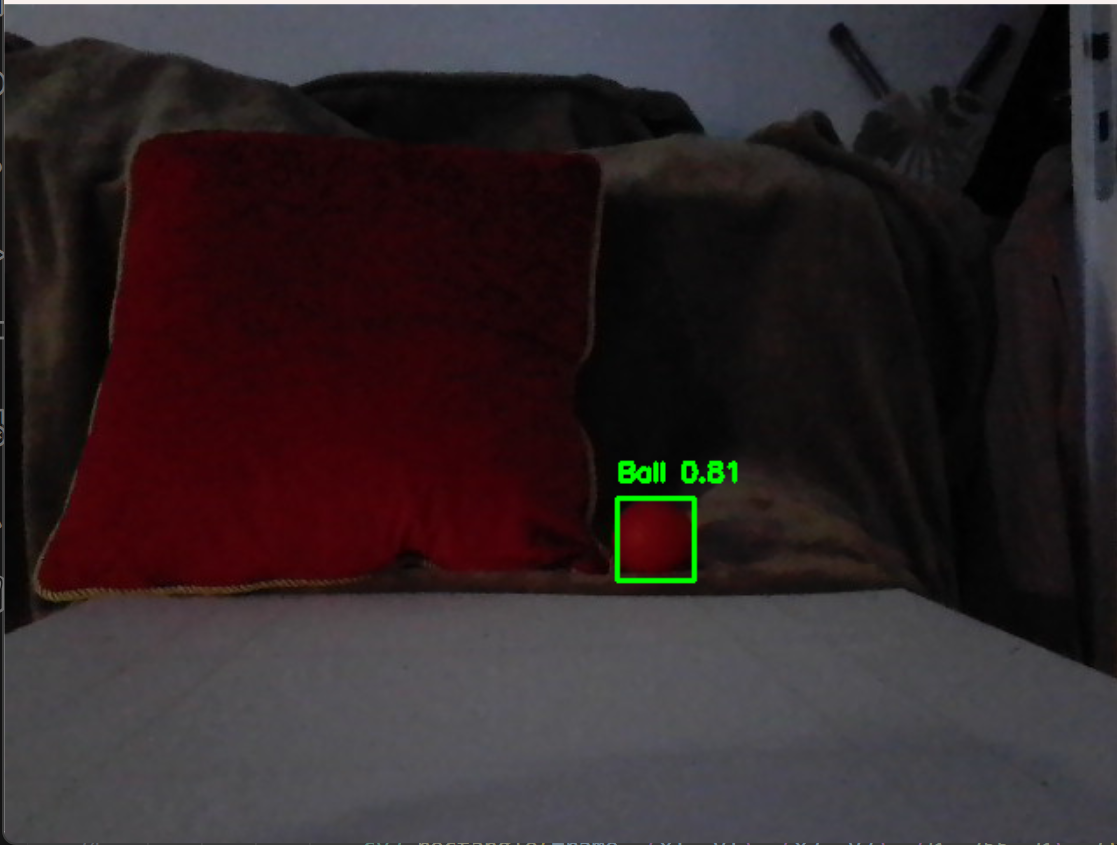
\includegraphics[width=0.6\textwidth]{Images/Porownanie/Yolo7 robot/Zrzut ekranu 2025-01-02 194641.png}
    \caption{Działanie modelu YOLOv7 przy złym oświetleniu - prawidłowa detekcja tylko pożądanego obiektu jakim jest piłka.}
    \label{fig:yolov7_bad_light_good_object}
\end{figure}

\newpage
\subsection{Charakterystyka modelu YOLOv8}

YOLOv8, będący nowocześniejszą wersją od YOLOv7, charakteryzuje się najwyższą precyzją detekcji spośród analizowanych algorytmów. W warunkach dobrego oświetlenia algorytm osiąga zadowalające wyniki, co zostało przedstawione na \textbf{Rysunku}~\ref{fig:yolov8_good_light}, gdzie obiekt został prawidłowo zidentyfikowany. 

W trudniejszych warunkach, takich jak gorsze oświetlenie, YOLOv8 wciąż jest w stanie poprawnie wykrywać obiekt o ściśle określonych cechach. Przykład działania algorytmu w takich warunkach zaprezentowano na \textbf{Rysunku}~\ref{fig:yolov8_bad_light}. 
\begin{figure}[h]
    \centering
    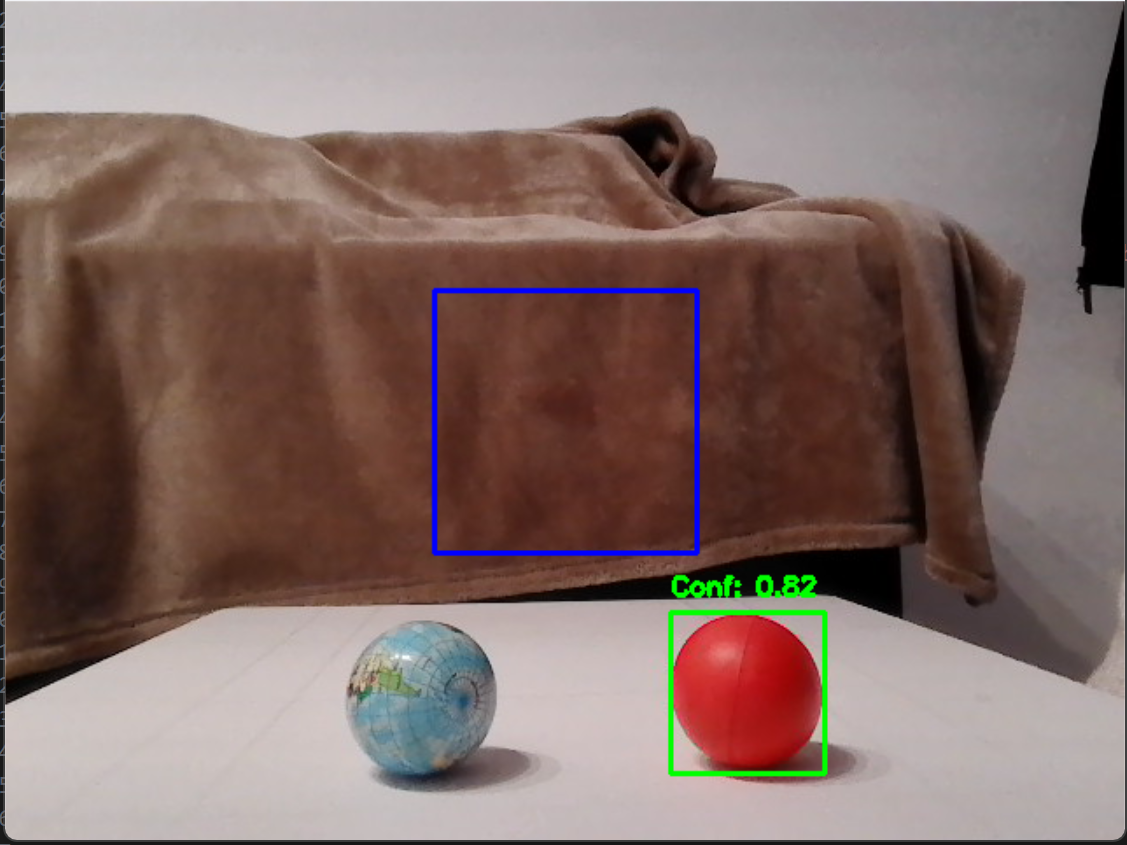
\includegraphics[width=0.6\textwidth]{Images/Porownanie/Yolo 8 laptop/Zrzut ekranu 2025-01-04 181013.png}
    \caption{Działanie modelu YOLOv8 przy dobrym oświetleniu - poprawna identyfkacja pożądanego obiektu.}
    \label{fig:yolov8_good_light}
\end{figure}

\begin{figure}[h]
    \centering
    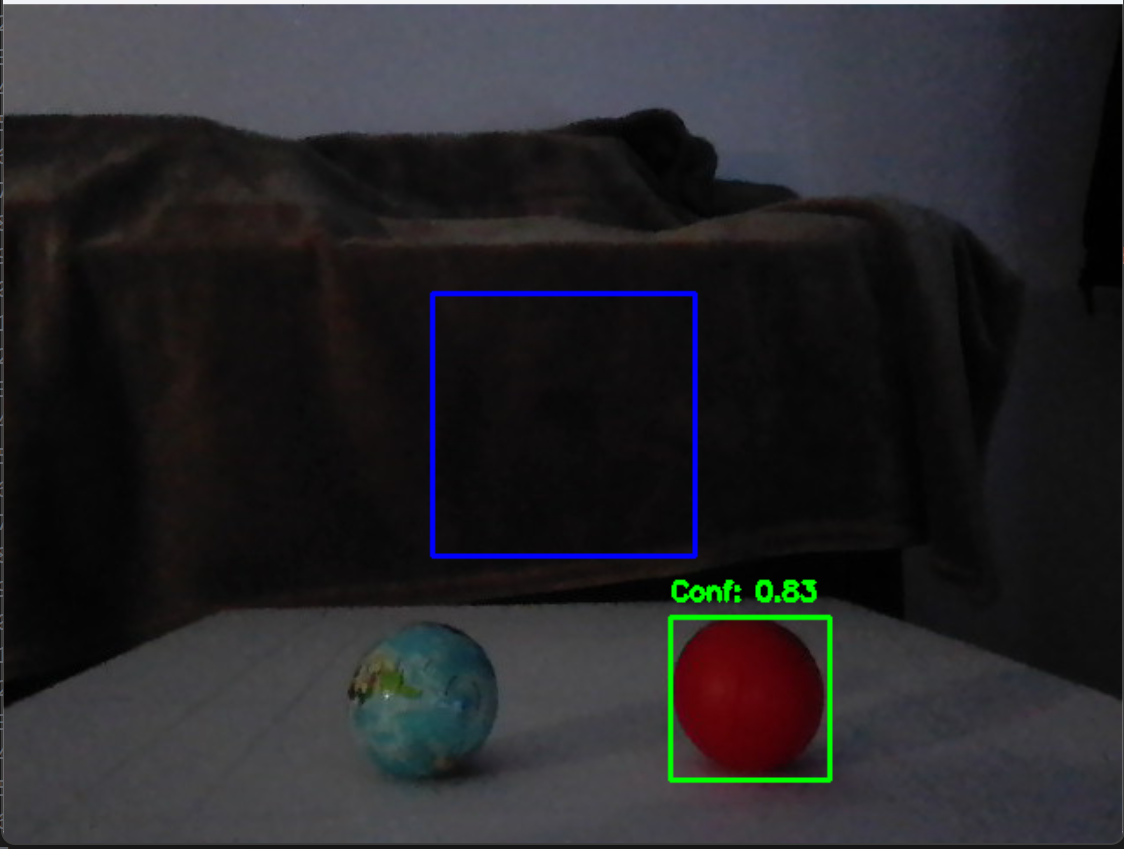
\includegraphics[width=0.6\textwidth]{Images/Porownanie/Yolo 8 laptop/Zrzut ekranu 2025-01-04 181029.png}
    \caption{Działanie modelu YOLOv8 przy gorszym oświetleniu - poprawna identyfikacja pożądanego obiektu.}
    \label{fig:yolov8_bad_light}
\end{figure}
\newpage

Pomimo wysokiej dokładności, YOLOv8 czasami błędnie identyfikuje obiekty. \textbf{Rysunek}~\ref{fig:yolov8_good_light_bad_object} przedstawia przykład, w którym w warunkach dobrego oświetlenia algorytm błędnie zidentyfikował czerwoną poduszkę jako obiekt piłkopodobny.

Z kolei \textbf{Rysunek}~\ref{fig:yolov8_good_light_good_object} pokazuje przypadek, w którym algorytm prawidłowo pominął obiekt w warunkach słabego oświetlenia. Może to być skutkiem zaniku barwy czerwonej w wyniku pogorszenia światła otoczenia.

\begin{figure}[h]
    \centering
    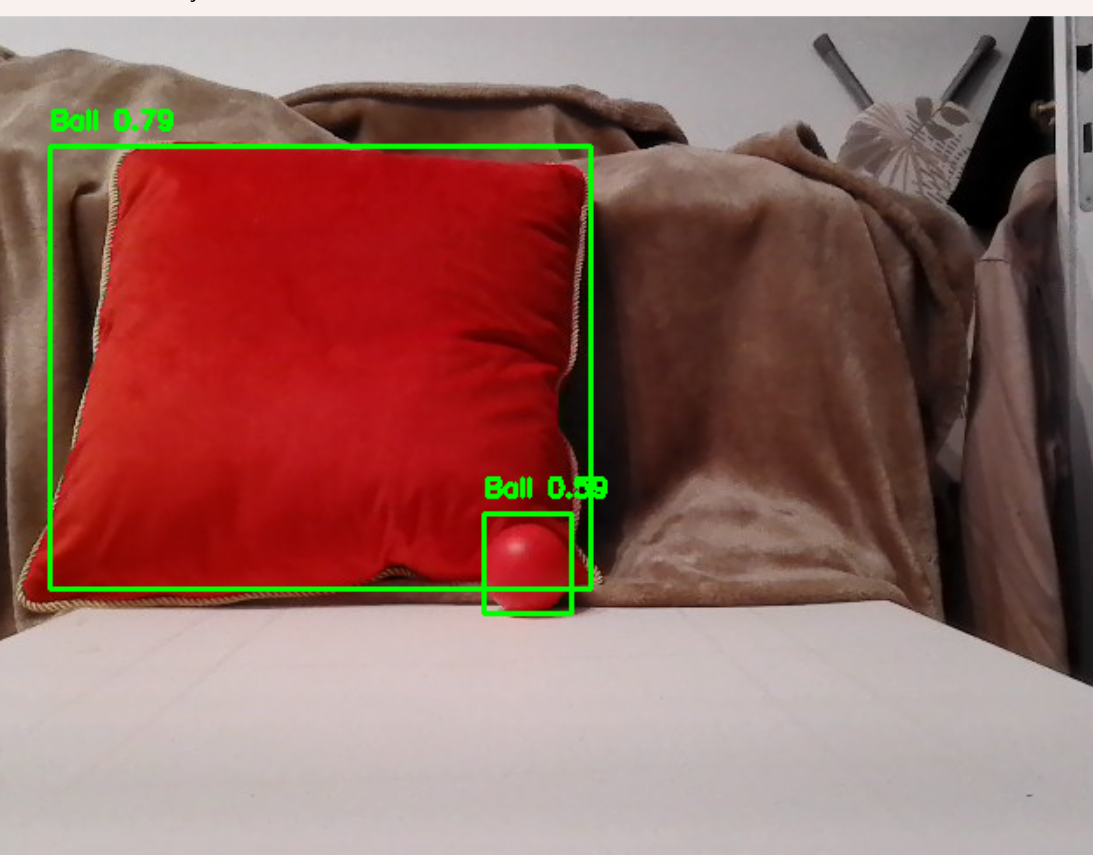
\includegraphics[width=0.6\textwidth]{Images/Porownanie/Yolo 8 laptop/Zrzut ekranu 2025-01-02 194808.png}
    \caption{Działanie modelu YOLOv8 przy dobrym oświetleniu - niepoprawne wykrycie przeszkody jako obiekt piłkopodobny.}
    \label{fig:yolov8_good_light_bad_object}
\end{figure}

\begin{figure}[h]
    \centering
    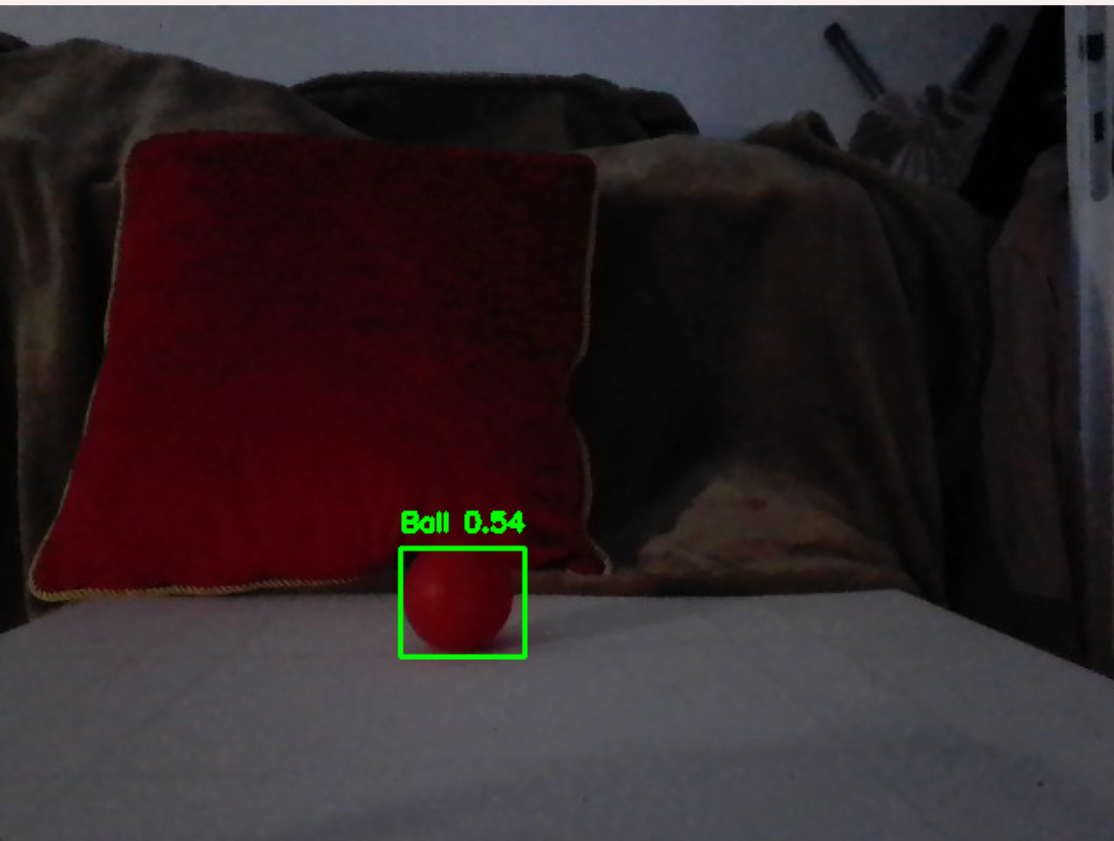
\includegraphics[width=0.6\textwidth]{Images/Porownanie/Yolo 8 laptop/Zrzut ekranu 2025-01-02 194704.png}
    \caption{Działanie modelu YOLOv8 przy gorszym oświetleniu - prawidłowe pominięcie obiektu będącego przeszkodą.}
    \label{fig:yolov8_good_light_good_object}
\end{figure}

\newpage
\subsection{Charakterystyka algorytmu binaryzacji}

Algorytm binaryzacji oparty na prostej segmentacji obrazu w przestrzeni barw HSV, na Raspberry Pi osiąga poziom nawet 25-30 FPS. Dzięki swej prostocie algorytm jest szczególnie efektywny w warunkach dobrego oświetlenia, jak pokazano na \textbf{Rysunku}~\ref{fig:binary_confusion_goodlight}.
W warunkach słabego oświetlenia, przedstawionych na \textbf{Rysunku}~\ref{fig:binary_confusion_badlight}, algorytm nadal jest w stanie poprawnie zidentyfikować obiekt. 

\begin{figure}[h]
    \centering
    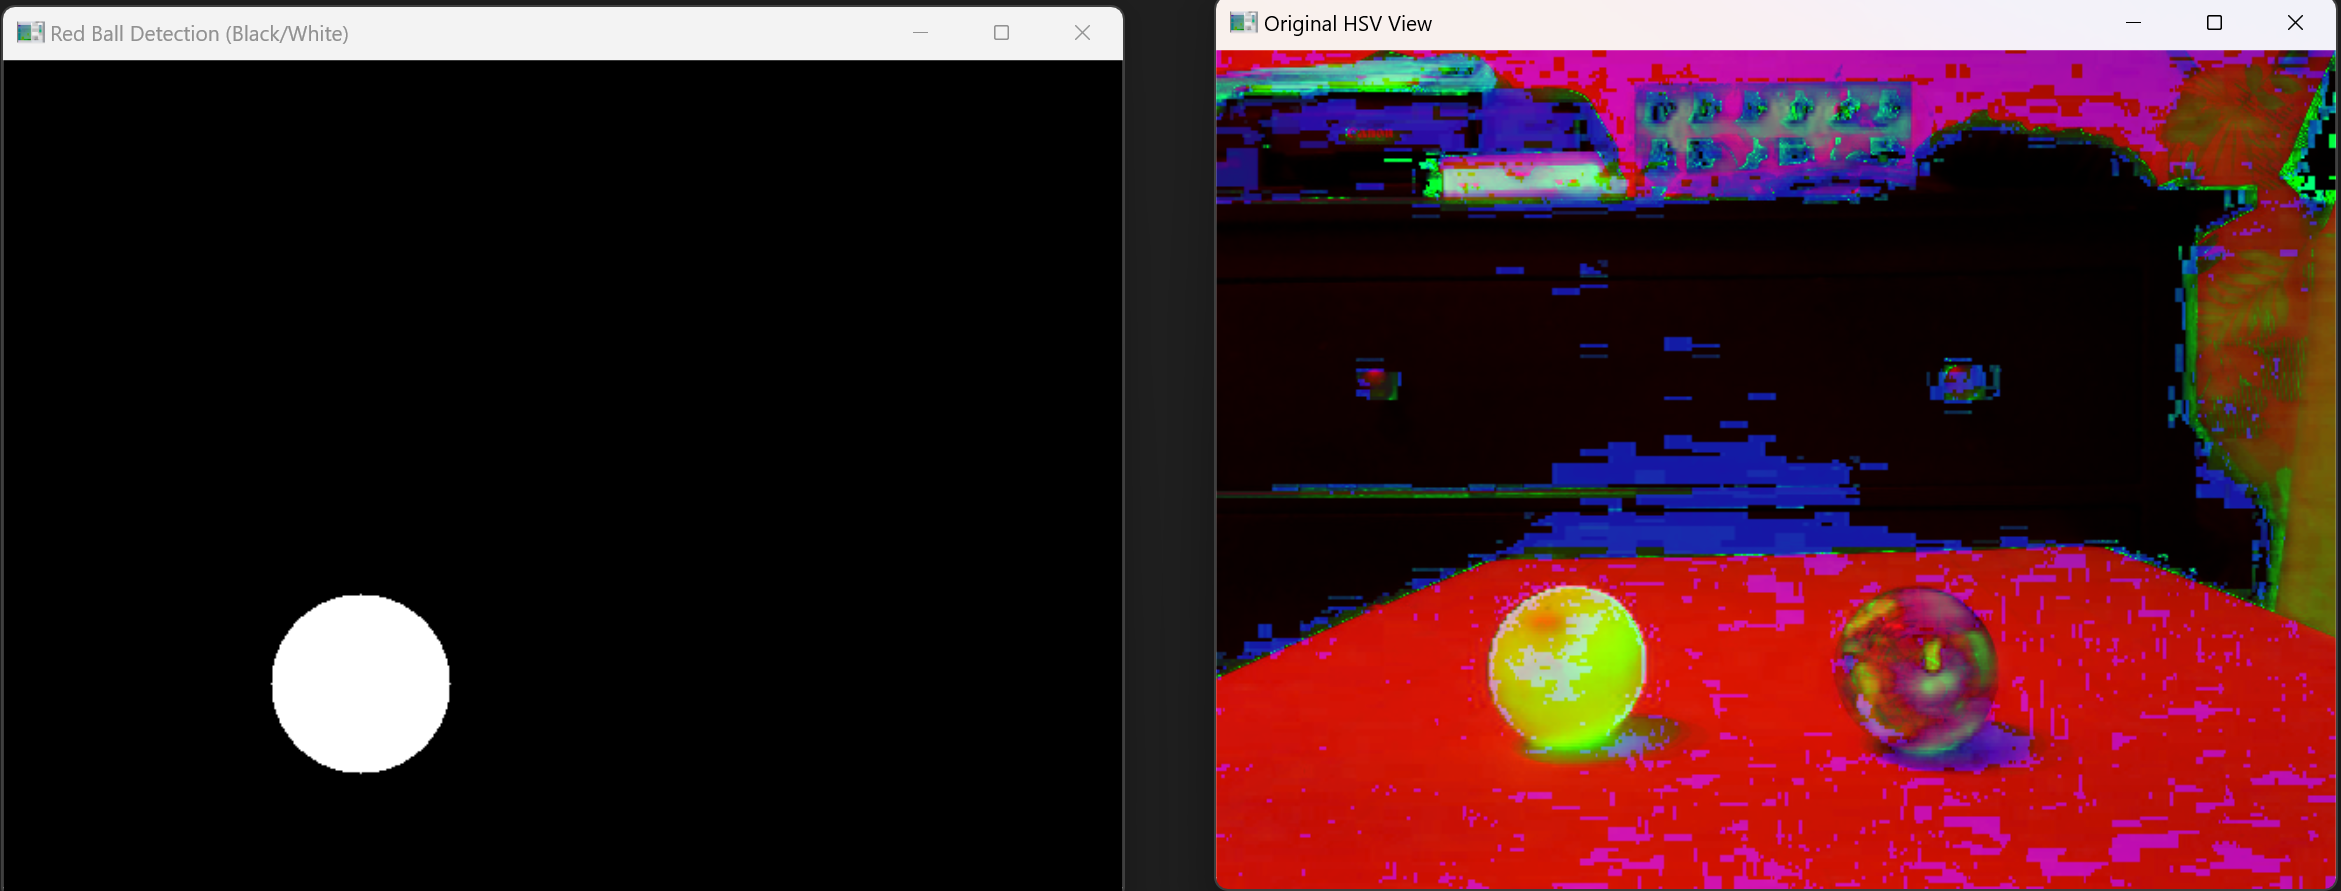
\includegraphics[width=0.8\textwidth]{Images/Porownanie/Binaryzacja/Zrzut ekranu 2025-01-02 194021.png}
    \caption{Działanie binaryzacji w warunkach dobrego oświetlenia.}
    \label{fig:binary_confusion_goodlight}
\end{figure}

\begin{figure}[h]
    \centering
    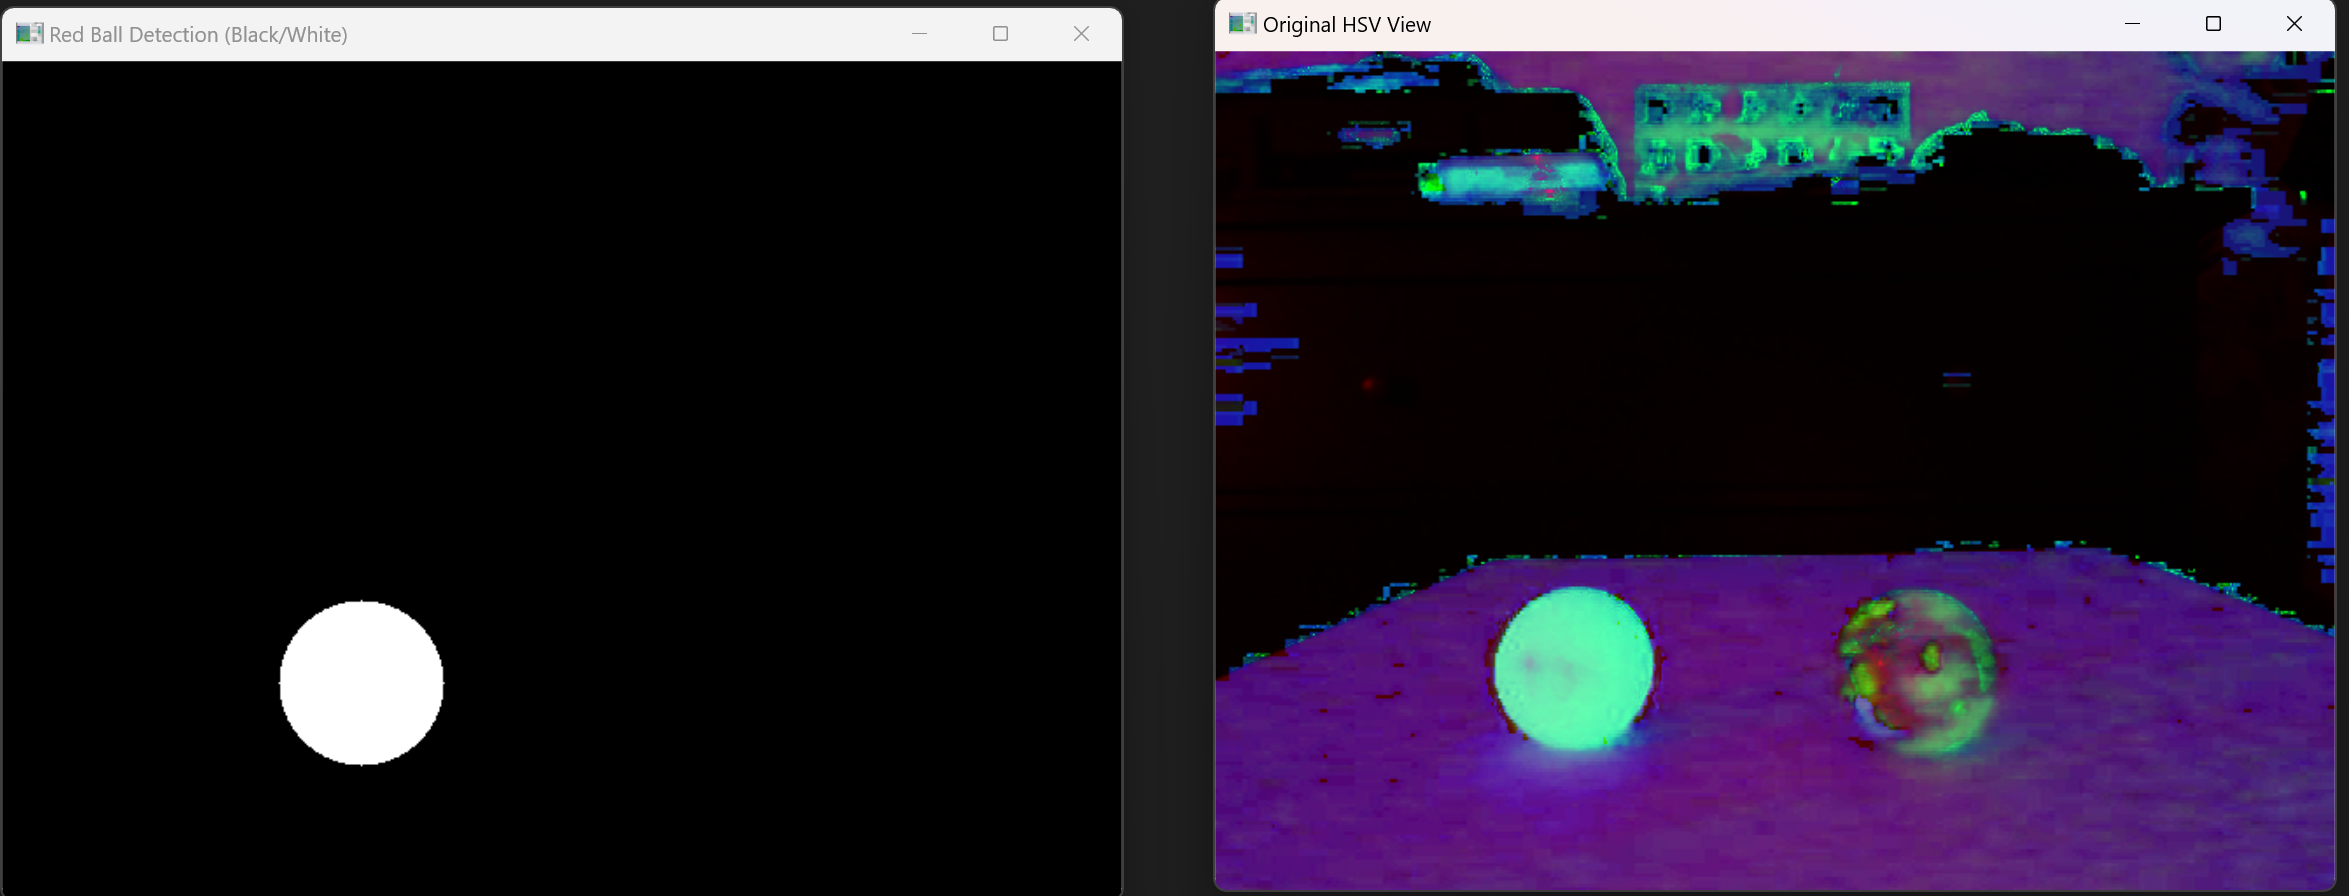
\includegraphics[width=0.8\textwidth]{Images/Porownanie/Binaryzacja/Zrzut ekranu 2025-01-02 194004.png}
    \caption{Działanie binaryzacji w warunkach słabego oświetlenia.}
    \label{fig:binary_confusion_badlight}
\end{figure}

\newpage

Jednakże, w bardziej złożonych sytuacjach, binaryzacja ujawnia swoje ograniczenia, co zilustrowano na \textbf{Rysunkach}~\ref{fig:binary_confusion_badlight_goodobject} i~\ref{fig:binary_confusion_goodlight_badobject}. W szczególności, w sytuacjach, gdy kolor obiektu zbliża się do kolorystyki tła, algorytm może błędnie klasyfikować obiekty.

\begin{figure}[h]
    \centering
    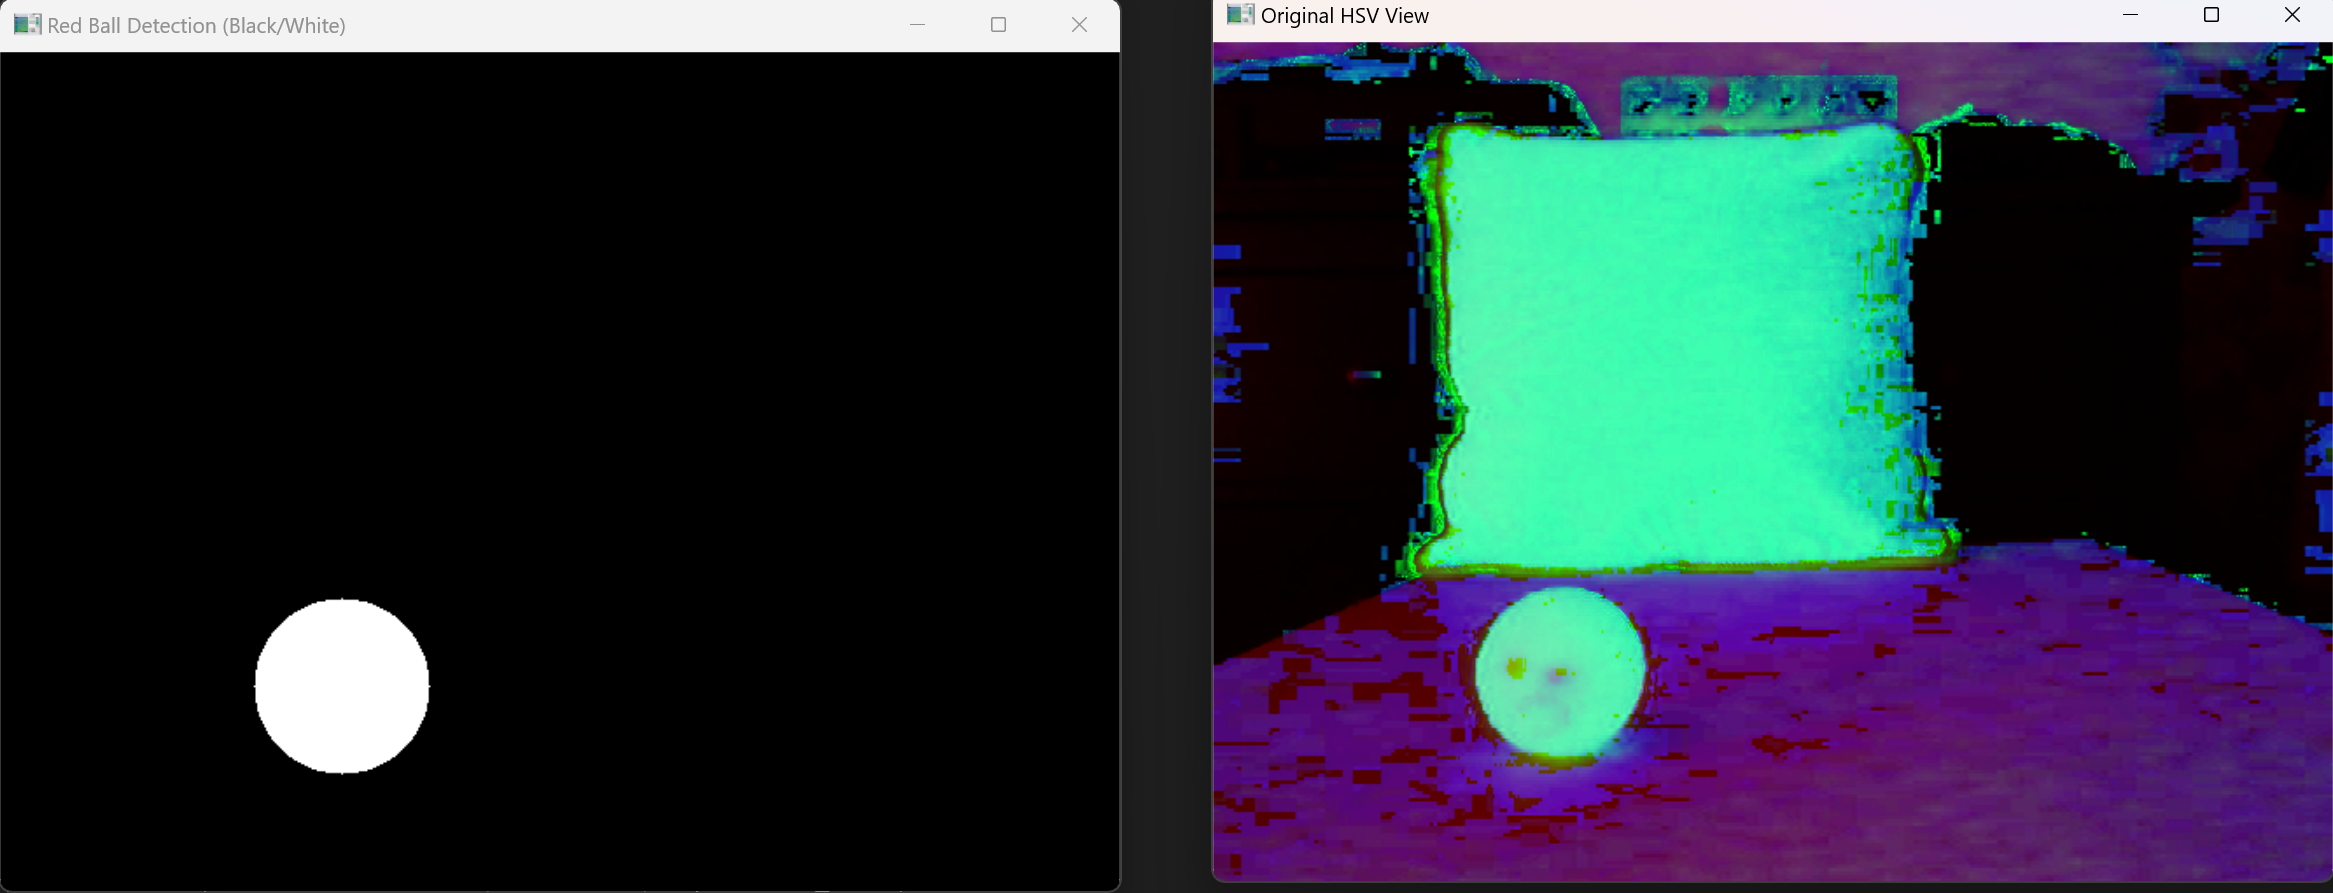
\includegraphics[width=0.8\textwidth]{Images/Porownanie/Binaryzacja/Zrzut ekranu 2025-01-02 193840.png}
    \caption{Działanie algorytmu binaryzacji w warunkach słabego oświetlenia - prawidłowe zignorowanie przeszkody.}
    \label{fig:binary_confusion_badlight_goodobject}
\end{figure}

\begin{figure}[h]
    \centering
    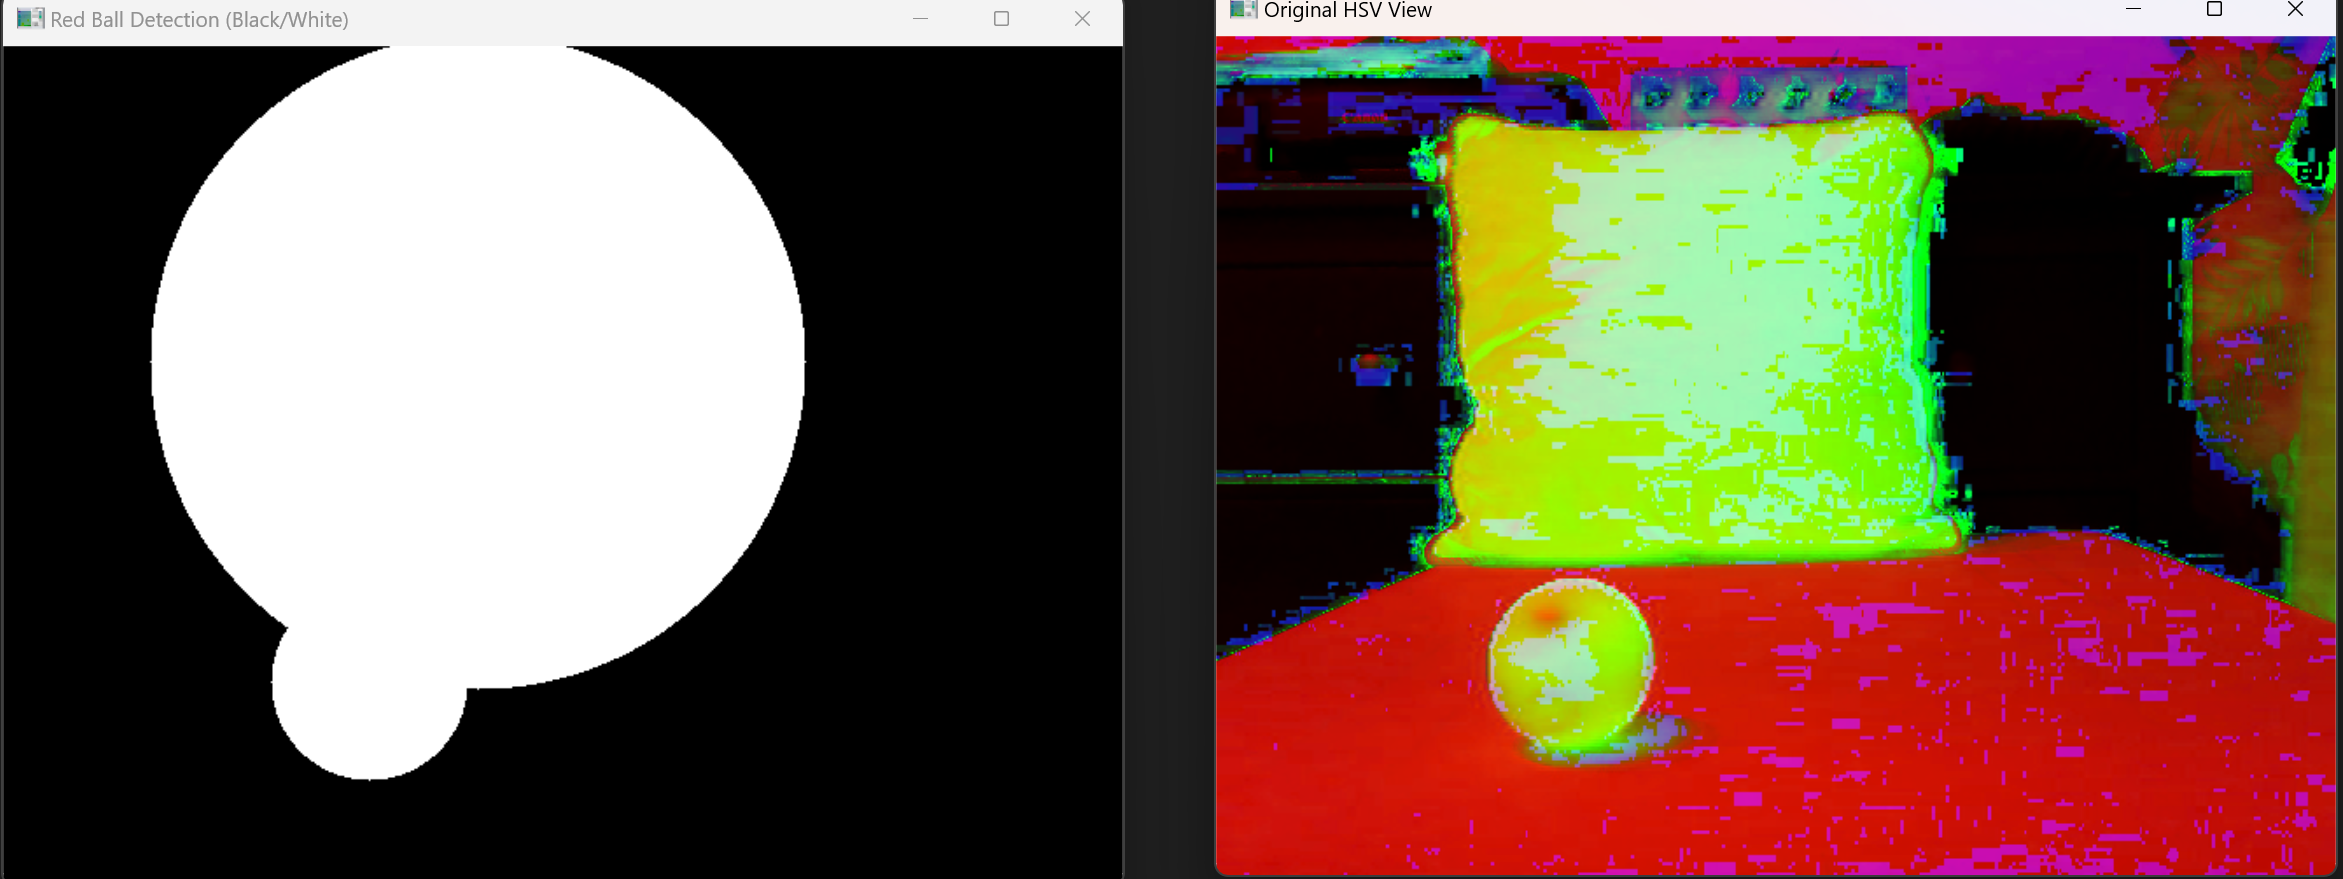
\includegraphics[width=0.8\textwidth]{Images/Porownanie/Binaryzacja/Zrzut ekranu 2025-01-02 193858.png}
    \caption{Działanie algorytmu binaryzacji w warunkach słabego oświetlenia - błędna detekcja przeszkody.}
    \label{fig:binary_confusion_goodlight_badobject}
\end{figure}

Algorytm binaryzacji wyróżnia się wysoką szybkością działania, co czyni go dobrym rozwiązaniem w systemach o ograniczonych zasobach obliczeniowych. Niemniej jednak, jego skuteczność zależy w dużej mierze od precyzyjnego doboru zakresów wartości HSV oraz warunków otoczenia.


\newpage
\subsection{Wnioski}

\paragraph{Działanie na komputerze osobistym}
Jak przedstawiono w \textbf{Tabelach}~\ref{tab:bez_przeszkody} i~\ref{tab:z_przeszkoda}, algorytmy detekcji różniły się skutecznością w zależności od warunków oświetleniowych i obecności przeszkód. 

Algorytm \textbf{YOLOv7} osiągnął dobrą równowagę między szybkością a dokładnością, niezależnie od warunków oświetleniowych i przeszkód, stabilnie działając z prędkością 16.09 FPS. \textbf{YOLOv8} wyróżniał się najwyższą dokładnością, jednak kosztem niższej szybkości, osiągając 10.71 FPS. W przypadku scen z przeszkodami miał trudności z ich ignorowaniem w dobrym oświetleniu. \textbf{Binaryzacja}, choć najszybsza z algorytmów (29.61 FPS), miała trudności z prawidłową klasyfikacją obiektów w złożonych scenach, co może prowadzić do fałszywych detekcji.

\begin{table}[h!]
    \centering
    \caption{Wyniki algorytmów detekcji obiektu bez przeszkody w różnych warunkach oświetleniowych na komputerze osobistym.}
    \label{tab:bez_przeszkody}
    \begin{tabular}{lcccc}
    \toprule
     & \multicolumn{2}{c}{Dobre oświetlenie} & \multicolumn{2}{c}{Złe oświetlenie} \\
    \cmidrule(r){2-3} \cmidrule(r){4-5}
    Algorytm & Czy wykryto & FPS & Czy wykryto & FPS \\
    \midrule
    YOLOv7 & TAK & 16.09 & TAK & 16.09 \\
    YOLOv8 & TAK & 10.71 & TAK & 10.71 \\
    Binaryzacja & TAK & 29.61 & TAK & 29.61 \\
    \bottomrule
    \end{tabular}
\end{table}

\begin{table}[h!]
    \centering
    \caption{Wyniki algorytmów detekcji obiektu z przeszkodą w różnych warunkach oświetleniowych na komputerze osobistym.}
    \label{tab:z_przeszkoda}
    \begin{tabular}{lcccc}
    \toprule
     & \multicolumn{2}{c}{Dobre oświetlenie} & \multicolumn{2}{c}{Złe oświetlenie} \\
    \cmidrule(r){2-3} \cmidrule(r){4-5}
    Algorytm & Czy pominął przeszkodę & FPS & Czy pominął przeszkodę & FPS \\
    \midrule
    YOLOv7 & TAK & 16.09 & TAK & 16.09 \\
    YOLOv8 & NIE & 10.71 & TAK & 10.71 \\
    Binaryzacja & NIE & 29.61 & TAK & 29.61 \\
    \bottomrule
    \end{tabular}
\end{table}

\newpage

\paragraph{Działanie na Raspberry Pi}
Jak przedstawiono w \textbf{Tabelach}~\ref{tab:bez_przeszkody_rpi} i~\ref{tab:z_przeszkoda_rpi}, działanie algorytmów na Raspberry Pi było ograniczone przez mniejsze zasoby obliczeniowe. 

\textbf{YOLOv7} działał stabilnie z prędkością około 2.8 FPS, zachowując swoją skuteczność w ignorowaniu przeszkód oraz wykrywaniu obiektów w różnych warunkach oświetleniowych. \textbf{YOLOv8}, choć nadal dokładny, wykazał najniższą wydajność na Raspberry Pi, osiągając zaledwie 1.24 FPS. Algorytm \textbf{binaryzacji}, pomimo najwyższej szybkości działania 25.95 FPS, dokonywał nieprawidłowej detekcji obiektów w słabym oświetleniu, co ujawnia jego ograniczenia w bardziej wymagających warunkach.

\begin{table}[h!]
    \centering
    \caption{Wyniki algorytmów detekcji obiektu bez przeszkody w różnych warunkach oświetleniowych na Raspberry Pi.}
    \label{tab:bez_przeszkody_rpi}
    \begin{tabular}{lcccc}
    \toprule
     & \multicolumn{2}{c}{Dobre oświetlenie} & \multicolumn{2}{c}{Złe oświetlenie} \\
    \cmidrule(r){2-3} \cmidrule(r){4-5}
    Algorytm & Czy wykryto & FPS & Czy wykryto & FPS \\
    \midrule
    YOLOv7 & TAK & 2.80 & TAK & 2.70 \\
    YOLOv8 & TAK & 1.24 & TAK & 1.24 \\
    Binaryzacja & TAK & 25.95 & NIE & 12.49 \\
    \bottomrule
    \end{tabular}
\end{table}

\begin{table}[h!]
    \centering
    \caption{Wyniki algorytmów detekcji obiektu z przeszkodą w różnych warunkach oświetleniowych na Raspberry Pi.}
    \label{tab:z_przeszkoda_rpi}
    \begin{tabular}{lcccc}
    \toprule
     & \multicolumn{2}{c}{Dobre oświetlenie} & \multicolumn{2}{c}{Złe oświetlenie} \\
    \cmidrule(r){2-3} \cmidrule(r){4-5}
    Algorytm & Czy pominął przeszkodę & FPS & Czy pominął przeszkodę & FPS \\
    \midrule
    YOLOv7 & TAK & 2.80 & TAK & 2.70 \\
    YOLOv8 & NIE & 1.24 & NIE & 1.24 \\
    Binaryzacja & NIE & 25.95 & TAK & 12.49 \\
    \bottomrule
    \end{tabular}
\end{table}

Podsumowując, wybór algorytmu powinien być uzależniony od specyficznych wymagań aplikacji oraz dostępnych zasobów sprzętowych:
\begin{itemize}
    \item \textbf{YOLOv7} jest najlepszym wyborem dla aplikacji wymagających równowagi między dokładnością a szybkością, szczególnie na urządzeniach o ograniczonej mocy obliczeniowej, takich jak Raspberry Pi.
    \item \textbf{YOLOv8} nadaje się do aplikacji, gdzie priorytetem jest maksymalna dokładność, a ograniczenia sprzętowe są mniej istotne.
    \item \textbf{Binaryzacja} jest idealnym rozwiązaniem dla systemów wymagających bardzo szybkiego przetwarzania w czasie rzeczywistym, pod warunkiem, że scena jest dobrze oświetlona i nie zawiera przeszkód o podobnym kolorze.
\end{itemize}

\chapter{Napotkane problemy i ich rozwiązania}
\label{ch:06}
W niniejszym rozdziale przedstawiono i opisano problemy związane z realizacją projektu oraz zaproponowane rozwiązania, które pozwoliły na skuteczne zaimplementowanie systemu wizyjnego dla robota mobilnego. Omówiono wyzwania związane z wyborem algorytmów detekcji obiektów, implementacją algorytmów śledzenia obiektu oraz elektroniką i mechaniką robota.

\section{Wybór algorytmów detekcji obiektów}

Pierwszym wyzwaniem w realizacji projektu było dokonanie wyboru odpowiedniego modelu głębokiego uczenia oraz przygotowanie zbioru danych do treningu. Początkowo założono, że model YOLO zostanie wytrenowany na komputerze osobistym. Jednak podczas konfiguracji napotkano trudności związane z integracją bibliotek, co uniemożliwiło rozpoczęcie procesu treningowego. W odpowiedzi na te problemy podjęto próbę zastosowania alternatywnego rozwiązania w postaci TensorFlow. Niestety, wymagało to stworzenia dedykowanego programu do treningu sieci neuronowej, co okazało się zbyt złożone i nieefektywne.

Przełom nastąpił dzięki wykorzystaniu platformy Roboflow, która umożliwiła intuicyjne etykietowanie obrazów i przygotowanie zestawu danych.

Aby przyspieszyć proces treningu modelu, zdecydowano się na wykorzystanie platformy Google Colab, zapewniającej dostęp do jednostek GPU. Po zakończeniu treningu modelu plik \texttt{best.pt} został pobrany. Próba uruchomienia modelu na komputerze osobistym początkowo nie powiodła się z powodu brakujących folderów \texttt{utils} oraz \texttt{models}, w tym pliku \texttt{experimental.py}. Dopiero po odpowiedniej konfiguracji środowiska i wskazaniu właściwych ścieżek model został pomyślnie uruchomiony na komputerze osobistym.

Kolejnym wyzwaniem było dostosowanie modelu do pracy na platformie Raspberry Pi, gdzie zasoby sprzętowe są ograniczone. YOLOv7 działał na tej platformie z prędkością zaledwie 2–3 FPS, co okazało się niewystarczające. W odpowiedzi podjęto próbę wytrenowania modelu YOLOv8 i przekonwertowania go za pomocą ONNX na TensorFlow Lite. Choć konwersja pozwoliła na osiągnięcie prędkości 10 FPS, spowodowała znaczną utratę jakości detekcji, przez co robot nie był w stanie skutecznie wykrywać piłki. Dla porównania, uruchomienie YOLOv8 bez konwersji dawało prędkość jedynie 0.9–1.2 FPS, co było najgorszym wynikiem spośród testowanych rozwiązań.

Ostatecznie zdecydowano się pozostać przy modelu YOLOv7, pomimo ograniczonej prędkości wynoszącej 3 FPS. Rozważano również zastosowanie starszych wersji YOLO, które mogłyby lepiej sprawdzić się na platformie Raspberry Pi, jednak komplikacje związane z implementacją spowodowały rezygnację z tego kierunku działań.


\section{Implementacja algorytmów śledzenia obiektu}

Jednym z największych wyzwań podczas realizacji projektu było zaimplementowanie wytrenowanego modelu, przygotowanego na komputerze osobistym z systemem Windows, na platformie Raspberry Pi.

Pierwszym problemem napotkanym podczas implementacji był błąd przy instalacji biblioteki PyTorch. Kluczowym rozwiązaniem okazało się przejście na 64-bitową wersję systemu Raspberry Pi OS, ponieważ wersja 32-bitowa nie była kompatybilna z wymaganą wersją biblioteki. Po instalacji odpowiedniej wersji systemu i zaktualizowaniu biblioteki PyTorch, przystąpiono do przesłania niezbędnych plików na Raspberry Pi za pomocą protokołu SSH.

Kolejnym wyzwaniem było uruchomienie programu detekcji na Raspberry Pi. Podczas próby wczytania modelu pojawił się błąd związany z funkcją \texttt{attempt\_download(w)} w pliku \texttt{experimental.py}. Funkcja ta, odpowiedzialna za automatyczne pobieranie brakujących wag modelu z sieci, powodowała problemy w środowisku Raspberry Pi, gdzie lokalne wagi były już dostępne. Aby rozwiązać ten problem, zdecydowano się na usunięcie tej linii kodu. 

Zmodyfikowany fragment pliku przedstawiono poniżej:
\begin{lstlisting}[language=Python, caption={Usunięcie funkcji \texttt{attempt\_download} z pliku \texttt{experimental.py}.}, label={lst:attempt_download_removal}, captionpos=b]
attempt_download(w)
\end{lstlisting}

Dzięki tej modyfikacji program poprawnie wczytywał lokalnie przechowywane wagi modelu bez potrzeby ponownego pobierania ich z sieci.

Po udanej modyfikacji programu pojawił się jednak problem związany z wyświetlaniem obrazu z kamery. Zakładano, że podgląd wideo będzie realizowany na komputerze za pomocą protokołu VNC. Okazało się jednak, że jednoczesne korzystanie z bibliotek \texttt{libcamera} i \texttt{OpenCV} powodowało konflikty, które uniemożliwiały wyświetlenie okna podglądu w czasie rzeczywistym. 

Ostatecznie zrezygnowano z podglądu obrazu, ograniczając program do wyświetlania w konsoli informacji o wykryciu obiektów, liczbie przetworzonych klatek na sekundę (FPS) oraz aktualnych pozycjach serwomechanizmów. Takie rozwiązanie, choć nieidealne, pozwoliło na uruchomienie programu i realizację podstawowej funkcjonalności systemu.


\section{Problemy związane z elektroniką i zasilaniem}

Kolejnym wyzwaniem w projekcie było zaprojektowanie odpowiedniego systemu zasilania dla Raspberry Pi. Początkowo planowano wykorzystanie dwóch ogniw o łącznym napięciu 7.2V jako źródła zasilania. Ze względu na to, że Raspberry Pi wymaga maksymalnego napięcia wynoszącego 5V, konieczne było zastosowanie przetwornicy typu \textit{step-down}, której zadaniem było obniżenie napięcia wejściowego do bezpiecznego poziomu.

Po podłączeniu dwóch ogniw do wejścia przetwornicy oraz kabla USB-C do jej wyjścia uzyskano stabilne napięcie 5V, co pozwoliło na uruchomienie Raspberry Pi. Problem pojawił się jednak podczas próby inicjalizacji modułu kamery. Okazało się, że natężenie prądowe dostarczane przez przetwornicę było zbyt niskie, aby zasilić jednocześnie system operacyjny i moduł kamery, co uniemożliwiało jej poprawne działanie.

W odpowiedzi na ten problem zastosowano przetwornicę o wyższej wydajności prądowej, zdolną dostarczyć do 3A. Niestety, rezultat okazał się podobny – natężenie nadal było niewystarczające, aby w pełni zasilić wszystkie komponenty systemu. Istnieje możliwość, że zastosowana przetwornica była wadliwa i nie dostarczała deklarowanego natężenia prądu, co mogło przyczynić się do problemów z zasilaniem.

Ostatecznie problem rozwiązano poprzez zastosowanie powerbanku jako źródła zasilania dla Raspberry Pi. Powerbank oferujący napięcie 5V i natężenie 3A zapewnił stabilne zasilanie zarówno dla Raspberry Pi, modułu kamery, jak i dwóch serwomechanizmów. Takie rozwiązanie pozwoliło na bezproblemową pracę całego systemu i wyeliminowało problemy związane z niedoborem natężenia prądu.


\newpage
\section{Problemy związane z mechaniką i sterowaniem}

Aby robot mobilny mógł skutecznie realizować swoje zadanie, kluczowe było zaimplementowanie modułu śledzącego obiekt. Początkowo zakładano statyczne umieszczenie kamery, a śledzenie czerwonej piłki miało być realizowane poprzez obrót całej platformy jeżdżącej. Rozwiązanie to okazało się niepraktyczne i mało efektywne, dlatego zdecydowano się na alternatywę polegającą na poruszaniu samą kamerą.

Do realizacji tego zadania wykorzystano uchwyt na kamerę wyposażony w dwa serwomechanizmy: jeden odpowiedzialny za obrót kamery wokół osi pionowej (\textit{pan}), a drugi za obrót wokół osi poziomej (\textit{tilt}). Dzięki temu rozwiązaniu kamera mogła dynamicznie śledzić ruch obiektu, co znacząco zwiększyło jej pole widzenia.

\paragraph{Obrót obrazu i sterowanie serwomechanizmami} 
Ze względu na mechaniczne zamocowanie kamery, obraz z kamery był obrócony o 180°. Wymagało to dodatkowego przekształcenia obrazu w programie za pomocą funkcji \texttt{cv2.rotate(frame, cv2.ROTATE\_180)}.

Aby program mógł skutecznie śledzić obiekt, w centrum obrazu umieszczono kwadrat, który pełnił funkcję rozszerzonego centrum kadru. Jeśli obiekt znajdował się w granicach tego kwadratu, kamera nie wykonywała korekt, co zapobiegało drganiom oraz niestabilności wynikającym ze zmiennego oświetlenia. W przypadku, gdy obiekt przesuwał się poza centrum obrazu, obliczano przesunięcie względem środka kadru i na tej podstawie obliczano kąty wychylenia serwomechanizmów.

\paragraph{Zależność ruchu kamery i silników DC}
Zastosowanie serwomechanizmów pozwoliło uzależnić ruchy silników DC od kątów wychylenia kamery:
\begin{itemize}
    \item Robot pozostawał nieruchomy, gdy kąt pochylenia serwomechanizmu \textit{tilt} osiągał granicę \(-30^\circ\), co oznaczało, że wykryty obiekt znajdował się zbyt blisko.
    \item Robot poruszał się do przodu, gdy serwomechanizm \textit{tilt} znajdował się w pozycji powyżej \(-30^\circ\), wskazując na wprost.
    \item Robot skręcał w prawo lub w lewo, gdy serwomechanizm \textit{pan} przekraczał granice \(\pm 25^\circ\).
\end{itemize}

\paragraph{Mechanizm poszukiwania obiektu}
W sytuacji, gdy obiekt znajdował się poza polem widzenia kamery, zaimplementowano funkcję poszukiwania. W jej ramach serwomechanizmy wykonywały ruch eliptyczny, a kąty ich wychyleń były generowane na podstawie funkcji trygonometrycznych. Dzięki temu robot był w stanie skutecznie odnaleźć obiekt i kontynuować jego śledzenie.

% TODO
\chapter{Podsumowanie i wnioski}
\label{ch:07}

W ramach niniejszej pracy zrealizowano projekt systemu wizyjnego dla robota mobilnego, którego zadaniem było autonomiczne wykrywanie i śledzenie obiektów. W projekcie wykorzystano zarówno zaawansowane algorytmy głębokiego uczenia (YOLOv7 i YOLOv8), jak i klasyczne techniki przetwarzania obrazów, takie jak binaryzacja. System został przeanalizowany pod kątem skuteczności i wydajności w różnych warunkach oświetleniowych oraz na dwóch platformach sprzętowych: komputerze osobistym i Raspberry Pi.

Przeprowadzone testy wykazały, że każde z zastosowanych podejść posiada swoje mocne i słabe strony. Modele YOLO zapewniły wysoką precyzję detekcji w złożonych warunkach, jednak ich działanie było ograniczone przez zasoby obliczeniowe modułu Raspberry Pi. Z kolei algorytm binaryzacji charakteryzował się znacznie wyższą szybkością, ale jego skuteczność w trudniejszych warunkach była ograniczona.

\section{Wnioski}
Na podstawie przeprowadzonych badań można sformułować wnioski iż Modele YOLOv7 i YOLOv8 są odpowiednie do zastosowań wymagających wysokiej precyzji detekcji, szczególnie w złożonych środowiskach lecz ich głównym ograniczeniem jest wysokie zapotrzebowanie na zasoby sprzętowe. 
Natomiast algorytm binaryzacji jest wydajnym rozwiązaniem w prostych scenariuszach, gdzie kluczowa jest szybkość działania, a zasoby obliczeniowe są ograniczone. 
Podsumowując Raspberry Pi, pomimo swoich ograniczeń sprzętowych, może być skutecznie wykorzystywane jako platforma do detekcji obiektów w czasie rzeczywistym, szczególnie przy zastosowaniu zoptymalizowanych algorytmów.

\section{Perspektywy dalszych badań}
W przyszłości można rozważyć nozwuj systemu polegający na wdrożeniu hybrydowego podejścia, które łączy algorytmy głębokiego uczenia z klasycznymi technikami przetwarzania obrazu, aby wykorzystać ich wzajemne zalety. Bądź optymalizację modeli YOLO pod kątem działania na platformach o ograniczonych zasobach obliczeniowych, na przykład poprzez wykorzystanie starszych wersji modeli albo wykorzystanie innych technik detekcji jak na przykład TensorFlow Lite. 









\backmatter

%\bibliographystyle{plplain}  % bibtex
%\bibliography{biblio} % bibtex
\printbibliography           % biblatex
\addcontentsline{toc}{chapter}{Bibliografia}

\begin{appendices}

% TODO
\chapter{Spis skrótów i symboli}

\begin{itemize}
\item[YOLO] algorytm głębokiego uczenia \english{You Only Look Once}
\item[HSV] przestrzeń barw \english{Hue, Saturation, Value}
\item[FPS] liczba klatek na sekundę \english{Frames Per Second}
\item[ONNX] otwarty format wymiany modeli uczenia maszynowego \english{Open Neural Network Exchange}
\item[VNC] narzędzie do zdalnego dostępu \english{Virtual Network Computing}
\item[SSH] protokół do zdalnego logowania \english{Secure Shell} 
\item[AGV] bezzałogowy pojazd jezdny \english{Autonomous Ground Vehicle}
\item[PLC] sterownik programowalny \english{Programmable Logic Controller}
\item[CCD] matryca światłoczuła \english{Charge-Coupled Device}
\item[GPS] system nawigacji satelitarnej \english{Global Positioning System}
\item[\(x_{\text{środek}}, y_{\text{środek}}\)] współrzędne środka obrazu.
\item[\(x_{\text{piłka}}, y_{\text{piłka}}\)] współrzędne środka obiektu.
\item[\(\Delta x, \Delta y\)] różnica między środkiem obrazu a środkiem obiektu.
\item[\(\theta_{\text{pan}}, \theta_{\text{tilt}}\)] kąty wychylenia serwomechanizmów (odpowiednio w płaszczyznach poziomej i pionowej).
\item[\(k_x, k_y\)] współczynniki skalujące szybkość korekcji.
\item[\(A_{\text{pan}}, A_{\text{tilt}}\)] amplitudy ruchu serwomechanizmów w poszczególnych płaszczyznach.
\item[\(\omega\)] prędkość kątowa.
\item[\(T\)] próg dla binaryzacji obrazu.
\item[\(J\)] wskaźnik jakości (funkcja kosztu w propagacji wstecznej).
\item[\(w_{ij}\)] waga sieci neuronowej między neuronami \(i\) i \(j\).
\item[\(\eta\)] współczynnik uczenia \english{Learning Rate}.     
\end{itemize}


% TODO
%\chapter{Źródła}
%
%Jeżeli w pracy konieczne jest umieszczenie długich fragmentów kodu źródłowego, należy je przenieść w to miejsce.


% % % % % % % % % % % % % % % % % % % % % % % % % % % % % % % % % % % 
% Pakiet minted wymaga odkomentowania w pliku config/settings.tex   %
% importu pakietu minted: \usepackage{minted}                       %
% i specjalnego kompilowania:                                       %
% pdflatex -shell-escape praca                                      %
% % % % % % % % % % % % % % % % % % % % % % % % % % % % % % % % % % % 

%\begin{minted}[linenos,breaklines,frame=lines]{c++}
%if (_nClusters < 1)
%   throw std::string ("unknown number of clusters");
%if (_nIterations < 1 and _epsilon < 0)
%   throw std::string ("You should set a maximal number of iteration or minimal difference -- epsilon.");
%if (_nIterations > 0 and _epsilon > 0)
%   throw std::string ("Both number of iterations and minimal epsilon set -- you should set either number of iterations or minimal epsilon.");
%\end{minted}


% TODO
\chapter{Lista dodatkowych plików, uzupełniających tekst pracy} 


W systemie do pracy dołączono dodatkowe pliki zawierające:
\begin{itemize}
    \item Pliki źródłowe programów uruchamianych na komputerze osobistym w folderze \texttt{Programy\_Komputer}
    \item Pliki źródłowe programów uruchamianych na Raspberry Pi w folderze \texttt{Programy\_Raspberry}
    \item Spis wymaganych bibliotek na RaspberryPi w pliku \texttt{Biblioteki.txt} 
    \item Film prezentujący działanie wizji robota mobilnego w pliku \texttt{Robot\_Wizja.mp4}
\end{itemize}


\listoffigures
\addcontentsline{toc}{chapter}{Spis rysunków}
\listoftables
\addcontentsline{toc}{chapter}{Spis tabel}

\end{appendices}

\end{document}


%% Finis coronat opus.

